\documentclass{article}

\usepackage[a4paper, total={6in, 8in}]{geometry}
\usepackage[utf8]{inputenc}

% Packages added by F. Key
\usepackage{amsmath}
\usepackage{amssymb}
\usepackage{authblk}
\usepackage{booktabs}
\usepackage{cleveref}
\usepackage{placeins}
\usepackage{todonotes}
\usepackage{tikz}
\usepackage{pgfplots}
\pgfplotsset{compat=1.17}
%\usepackage{showframe}
% GLOSSARIES
\usepackage[acronym,toc,nogroupskip]{glossaries}
%\makeglossaries
\begin{acronym}
    \acro{LDA}{\emph{Latent Dirichlet Allocation}}
    \acro{CMT}{\emph{Conference Management Toolkit}}
    \acro{TPMS}{\emph{The Toronto Paper Matching System}}
    \acro{MCMF}{\emph{MinCost-MaxFlow}}
\end{acronym}
% BIBLIOGRAPHY
\usepackage[url=false,eprint=false,giveninits=true]{biblatex} 
\addbibresource{bibliography.bib} 

%Packages added by M. v. Danwitz
\usepackage[font=footnotesize,labelfont=bf,position=bottom, skip=0.5ex]{subcaption}
\usepackage{siunitx}
\usepackage{tikz-dimline}

\title{Model Order Reduction for Deforming Domain Problems in a Time-Continuous Space-Time Setting}
\author[1,*]{Fabian Key}
\author[2]{Max von Danwitz}
\author[3]{Francesco Ballarin}
\author[4]{Gianluigi Rozza}
\affil[1]{Institute of Lightweight Design and Structural Biomechanics (ILSB), TU Wien, Vienna, Austria}
\affil[2]{Institute for Mathematics and Computer-Based Simulation (IMCS), Universität der Bundeswehr München, Neubiberg, Germany}
\affil[3]{Department of Mathematics and Physics, Università Cattolica del Sacro Cuore, Brescia, Italy}
%\affil[4]{Chair for Computational Analysis of Technical Systems (CATS), RWTH Aachen University, Aachen, Germany}
\affil[4]{Mathematics Area, mathLab, Scuola Internazionale Superiore di Studi Avanzati (SISSA), Trieste, Italy}

\date{}

\newcommand{\vek}[1]{\boldsymbol{#1}}
\newcommand{\mat}[1]{\boldsymbol{#1}}

\newcommand{\lp}{\left(}
\newcommand{\rp}{\right)}
\newcommand{\lb}{\left[}
\newcommand{\rb}{\right]}
% OPERATORS
% partial derivative
\newcommand{\dd}[2]{\frac{\partial#1}{\partial#2}}
% temporal derivative
\newcommand{\ddt}[1]{#1_t}
% divergence
\newcommand{\dv}[1]{\vek{\nabla} \cdot #1}
% gradient
\newcommand{\gr}[1]{\vek{\nabla} #1}
% Laplace
\newcommand{\lap}[1]{\vek{\Delta} #1}

% DOMAINS
\newcommand{\nsd}{n_{\text{sd}}}
\newcommand{\reals}{\mathbb{R}}
\newcommand{\realsSpace}{\reals^{\nsd}}
\newcommand{\domainSpace}[1][]{\Omega_{#1}}
\newcommand{\x}{\vek{x}}
\newcommand{\realsBoundarySpace}{\reals^{\nsd-1}}
\newcommand{\boundarySpace}{\Gamma}
\newcommand{\boundarySpaceDirichlet}{\boundarySpace_{\text{D}}}
\newcommand{\boundarySpaceNeumann}{\boundarySpace_{\text{N}}}
\newcommand{\On}{\Omega_{\text{n}}}
\newcommand{\timeInterval}{I}
\newcommand{\domainSpaceTime}{Q}
\newcommand{\boundarySpaceTime}{P}
\newcommand{\boundarySpaceTimeDirichlet}{\boundarySpaceTime_{\text{D}}}
\newcommand{\boundarySpaceTimeNeumann}{\boundarySpaceTime_{\text{N}}}
\newcommand{\domainSpaceTimeSlab}[1]{\domainSpaceTime_{#1}}
\newcommand{\boundarySpaceTimeSlab}[1]{\boundarySpaceTime_{#1}}
\newcommand{\boundarySpaceTimeSlabNeumann}[1]{\lp\boundarySpaceTimeNeumann\rp_{#1}}
\newcommand{\boundarySpaceTimeSlabDirichlet}[1]{\lp\boundarySpaceTimeDirichlet\rp_{#1}}
\newcommand{\realsSpaceTime}{\reals^{\nsd+1}}
\newcommand{\realsBoundarySpaceTime}{\reals^{\nsd}}
\newcommand{\xst}{\vek{x}^{\text{ST}}}
\newcommand{\nv}{\vek{n}}
\newcommand{\tv}{\vek{t}}

% INTEGRALS
%\newcommand{\intO}[2][]{\int_{\Omega^{#1}} #2 \ d\Omega}
%\newcommand{\intGN}[1]{\int_{\Gamma_{\text{N}}} #1 \ d\Gamma}
\newcommand{\intDomainSpaceTime}[1]{\int_{\domainSpaceTime} #1 \ d\domainSpaceTime}
\newcommand{\intElementSpaceTime}[1]{\int_{\domainSpaceTime^e}#1 \ d\domainSpaceTime}
\newcommand{\intElementSpaceTimeSlab}[2]{\int_{\domainSpaceTime^e_#1}#2 \ d\domainSpaceTime}
\newcommand{\intElementSpace}[1]{\int_{\domainSpace^e} #1 \ d\domainSpace}
\newcommand{\intBoundarySpace}[1]{\int_{\boundarySpace} #1 \ d\boundarySpace}
\newcommand{\intBoundarySpaceNeumann}[1]{\int_{\boundarySpaceNeumann} #1 \ d\boundarySpace}
\newcommand{\intBoundarySpaceTimeNeumann}[1]{\int_{\boundarySpaceTimeNeumann} #1 \ d\boundarySpaceTime}
\newcommand{\intDomainSpace}[1]{\int_{\domainSpace} #1 \ d\domainSpace}
\newcommand{\intDomainSpaceSlab}[2]{\int_{\domainSpace[#1]} #2 \ d\domainSpace}
% TIME
\newcommand{\tn}{t_n}
\newcommand{\timeStepSize}{\Delta t}

% FEM
\newcommand{\sobolevSpace}[1][]
{
    \ifthenelse{\equal{#1}{}}
        {\mathcal{H}^{1}}
        {\mathcal{H}^{1}\lp#1\rp}
}
\newcommand{\basisFunction}[1]{N_{#1}}
\newcommand{\nBasisFOM}{N{^{h}}}

\newcommand{\trialSpace}{\mathcal{S}}
\newcommand{\trialSpaceDiscrete}{\trialSpace^{h}}
\newcommand{\trial}{u}
\newcommand{\trialHom}{v}
\newcommand{\trialDiscrete}{\trial^{h}}
\newcommand{\trialHomDiscrete}{\trialHom^{h}}
\newcommand{\coeffTrialFOM}[1]{d_{#1}}
\newcommand{\lifting}{l}
\newcommand{\liftingDiscrete}{\lifting^{h}}
\newcommand{\basisFunctionLifting}{\basisFunction{\nBasisFOM+1}}
%\newcommand{\trialDiscreteSumHom}[1]{\sum_{#1=1}^{\nBasisFOM} \coeffTrialFOM{#1}\basisFunction{#1}}
\newcommand{\trialDiscreteSumHom}[1]{\sum_{#1\in\setNodesFree} \coeffTrialFOM{#1}\basisFunction{#1}}
\newcommand{\liftingDiscreteSum}[1]{\sum_{#1\in\setNodesDirichlet}\dval_{#1} \basisFunction{#1}}
\newcommand{\trialDiscreteSum}[1]{\trialDiscreteSumHom{#1}+\liftingDiscreteSum}

\newcommand{\weightingSpace}{\mathcal{V}}
\newcommand{\weightingSpaceDiscrete}{\weightingSpace^{h}}
\newcommand{\weight}{w}
\newcommand{\weightDiscrete}{\weight^{h}}
\newcommand{\coeffWeightFOM}[1]{c_{#1}}
%\newcommand{\weightDiscreteSum}[1]{\sum_{#1=1}^{\nBasisFOM}\coeffWeightFOM{#1}\basisFunction{#1}}
\newcommand{\weightDiscreteSum}[1]{\sum_{#1\in\setNodesFree}\coeffWeightFOM{#1}\basisFunction{#1}}

\newcommand{\bilinearFormDiffusion}[2]{a\left(#1,#2\right)}
\newcommand{\bilinearFormSource}[2]{\left(#1,#2\right)}
\newcommand{\bilinearFormNeumann}[2]{\left(#1,#2\right)_{\boundarySpaceNeumann}}
\newcommand{\bilinearFormNeumannSpaceTime}[2]{\left(#1,#2\right)_{\boundarySpaceTimeNeumann}}
\newcommand{\bilinearFormNeumannSpaceTimeParam}[3]{\left(#1,#2;#3\right)_{\boundarySpaceTimeNeumann}}
\newcommand{\mesh}{\mathcal{T}}
\newcommand{\setNodes}{\eta}
\newcommand{\setNodesDirichlet}{\eta_{D}}
\newcommand{\setNodesFree}{\bar{\eta}}
%\newcommand{\element}[1]{\mathcal{K}_{#1}}
\newcommand{\element}[1]{\domainSpace^{#1}}
\newcommand{\polynomialSpace}[1]{\mathcal{P}_{#1}}

\newcommand{\systemMatrixSymbol}{K}
\newcommand{\systemMatrix}{\mat{\systemMatrixSymbol}}
\newcommand{\systemMatrixEntry}[2]{\systemMatrixSymbol_{#1#2}}
\newcommand{\coeffTrialFOMVec}{\vek{d}}
\newcommand{\rhsVectorSymbol}{F}
\newcommand{\rhsVector}{\vek{\rhsVectorSymbol}}
\newcommand{\rhsVectorEntry}[1]{\rhsVectorSymbol_{#1}}
\newcommand{\rhsVectorLiftingSymbol}{G}
\newcommand{\rhsVectorLifting}{\vek{\rhsVectorLiftingSymbol}}
\newcommand{\rhsVectorLiftingEntry}[1]{\rhsVectorLiftingSymbol_{#1}}
% MATERIAL PROPERTIES
\newcommand{\density}{\rho}
\newcommand{\visc}{\eta}
% shear-thinning
\newcommand{\carreauA}{A}
\newcommand{\carreauB}{B}
\newcommand{\carreauC}{C}

% Parametric Stokes Equations
\newcommand{\param}{\mu}
\newcommand{\paramVec}{\vek{\param}}
\newcommand{\paramSpace}{\mathcal{D}}
\newcommand{\nParam}{P}
\newcommand{\realsParam}{\reals^{\nParam}}
\newcommand{\reynoldsNumber}{Re}
% velocity
\newcommand{\vel}{\vek{u}}
\newcommand{\velDirichlet}{\vel_{\text{D}}}
\newcommand{\velX}{u}
\newcommand{\velY}{v}
\newcommand{\velZ}{w}
\newcommand{\velTwoD}{\vel=(\velX,\velY)^{\text{T}}}
\newcommand{\velThreeD}{\vel=(\velX,\velY,\velZ)^{\text{T}}}
\newcommand{\testVel}{\vek{v}}
\newcommand{\trialSpaceVelocity}{\vek{\mathcal{S}}_{\vel}}
\newcommand{\trialSpaceVelocitySlab}[1]{\lp\trialSpaceVelocity\rp_{#1}}
\newcommand{\trialSpaceVelocityDiscrete}{\trialSpaceVelocity^h}
\newcommand{\trialSpaceVelocityDiscreteSlab}[1]{(\trialSpaceVelocityDiscrete)_{#1}}
\newcommand{\trialVelocity}{\vek{u}}
\newcommand{\trialVelocityParam}{\vek{u}\lp\paramVec\rp}
\newcommand{\trialVelocityDiscrete}{\trialVelocity^h}
\newcommand{\trialVelocityHom}{\vek{v}}
\newcommand{\trialVelocityHomDiscrete}{\trialVelocityHom^h}
\newcommand{\liftingVelocityDiscrete}{\vek{l}^h}
\newcommand{\weightingSpaceVelocity}{\vek{\mathcal{V}}_{\vel}}
\newcommand{\weightingSpaceVelocitySlab}[1]{\lp\weightingSpaceVelocity\rp_{#1}}
\newcommand{\weightingSpaceVelocityDiscrete}{\weightingSpaceVelocity^h}
\newcommand{\weightingSpaceVelocityDiscreteSlab}[1]{(\weightingSpaceVelocityDiscrete)_{#1}}
\newcommand{\weightVelocity}{\vek{w}}
\newcommand{\weightVelocityDiscrete}{\weightVelocity^h}
\newcommand{\sobolevSpaceVector}[1][]
{
    \ifthenelse{\equal{#1}{}}
        {\vek{\mathcal{H}}^1}
        {\vek{\mathcal{H}}^1\lp#1\rp}
}
\newcommand{\nBasisVelocityFOM}{N^{h}_{\vel}}
\newcommand{\coeffVelocityFOM}[1]{v_{#1}}
\newcommand{\basisFunctionVelocityFOM}[1]{\vek{N}^{\vel}_{#1}}
% pressure
\newcommand{\p}{p}
\newcommand{\testP}{q}
\newcommand{\trialSpacePressure}{\mathcal{S}_{\p}}
\newcommand{\trialSpacePressureSlab}[1]{\lp\trialSpacePressure\rp_{#1}}
\newcommand{\trialSpacePressureDiscrete}{\trialSpacePressure^h}
\newcommand{\trialSpacePressureDiscreteSlab}[1]{(\trialSpacePressureDiscrete)_{#1}}
\newcommand{\trialPressure}{p}
\newcommand{\trialPressureParam}{p\lp\paramVec\rp}
\newcommand{\trialPressureDiscrete}{\trialPressure^h}
\newcommand{\weightingSpacePressure}{\trialSpacePressure}
\newcommand{\weightingSpacePressureSlab}[1]{\lp\weightingSpacePressure\rp_{#1}}
\newcommand{\weightingSpacePressureDiscrete}{\weightingSpacePressure^h}
\newcommand{\weightingSpacePressureDiscreteSlab}[1]{(\weightingSpacePressureDiscrete)_{#1}}
\newcommand{\weightPressure}{q}
\newcommand{\weightPressureDiscrete}{\weightPressure^h}
\newcommand{\nBasisPressureFOM}{N^{h}_{\p}}
\newcommand{\coeffPressureFOM}[1]{p_{#1}}
\newcommand{\basisFunctionPressureFOM}[1]{N^{\p}_{#1}}
% Neumann values
\newcommand{\nval}{h}
% body force
\newcommand{\bdf}{\vek{f}}
% Cauchy stress tensor
\newcommand{\cstressSymbol}{\mat{\sigma}}
\newcommand{\cstress}[2]{\cstressSymbol\lp #1,#2 \rp}
\newcommand{\cstressParam}[2]{\cstressSymbol\lp #1,#2 ; \paramVec\rp}
\newcommand{\deviatoricStress}{\mat{\tau}}
\newcommand{\tractionNeumann}{\vek{h}}
% rate of strain tensor
\newcommand{\rosSymbol}{\mat{\epsilon}}
\newcommand{\ros}[1]{\rosSymbol\lp #1 \rp}
% shear rate
\newcommand{\shearrate}{\dot{\gamma}}
% bilinear forms
\newcommand{\bilinearFormViscousStress}[2]{a\lp #1 ,#2 \rp}
\newcommand{\bilinearFormPressure}[2]{b\lp #1, #2 \rp}
\newcommand{\bilinearFormPressureParam}[3]{b\lp #1, #2; #3 \rp}
\newcommand{\trilinearFormConvection}[3]{c\lp #1; #2, #3 \rp}
% stabilization
\newcommand{\weightMomentum}[3]{\mathcal{P}\lp#1,#2;#3\rp}
\newcommand{\residualMomentum}[2]{\mathcal{R}\lp#1,#2\rp}
\newcommand{\tMom}{\tau_{\textnormal{MOM}}\lp\trialVelocityDiscrete, \paramVec\rp}
\newcommand{\tMomPlain}{\tau_{\textnormal{MOM}}}
\newcommand{\tCon}{\tau_{\textnormal{CONT}}}
\newcommand{\bilinearFormStabMom}[4]
{
s_{\text{MOM}}\lp#1,#2,#3,#4\rp
}
\newcommand{\bilinearFormStabCon}[2]
{
s_{\text{CONT}}\lp#1,#2\rp
}
\newcommand{\bilinearFormStabMomStokes}[2]
{
s_{\text{MOM}}\lp#1,#2\rp
}
\newcommand{\bilinearFormStabMomStokesTemporal}[3]
{
s_{\text{MOM}}\lp#1,#2,#3\rp
}
%
\newcommand{\superscriptROM}{N}
\newcommand{\trialVelocityReduced}{\trialVelocity^{\superscriptROM}}
\newcommand{\trialVelocityHomDiscreteParam}{\trialVelocityHomDiscrete\lp\paramVec\rp}
\newcommand{\trialVelocityHomReduced}{\trialVelocityHom^{\superscriptROM}}
\newcommand{\trialVelocityHomReducedParam}{\trialVelocityHomReduced\lp\paramVec\rp}
\newcommand{\weightVelocityReduced}{\weightVelocity^{\superscriptROM}}
\newcommand{\trialPressureDiscreteParam}{\trialPressureDiscrete\lp\paramVec\rp}
\newcommand{\trialPressureReduced}{\trialPressure^{\superscriptROM}}
\newcommand{\trialPressureReducedParam}{\trialPressureReduced\lp\paramVec\rp}
\newcommand{\weightPressureReduced}{\weightPressure^{\superscriptROM}}

\newcommand{\bilinearFormViscousStressParam}[4]{a\lp #1 ,#2;#3, #4 \rp}
\newcommand{\bilinearFormStabMomStokesParam}[3]{s_{\text{MOM}}\lp#1,#2;#3\rp}

\newcommand{\matrixViscousStressSymbol}{A}
\newcommand{\matrixViscousStress}{\mat{\matrixViscousStressSymbol}}
\newcommand{\matrixViscousStressParam}{\matrixViscousStress\lp\trialVelocityDiscrete,\paramVec\rp}
\newcommand{\matrixPressureSymbol}{B}
\newcommand{\matrixPressure}{\mat{\matrixPressureSymbol}}
\newcommand{\matrixPressureTrans}{\matrixPressure^{\text{T}}}
\newcommand{\matrixStabMomStokesSymbol}{S}
\newcommand{\matrixStabMomStokes}{\mat{\matrixStabMomStokesSymbol}}
\newcommand{\matrixStabMomStokesParam}{\matrixStabMomStokes\lp\trialVelocityDiscrete,\paramVec\rp}
\newcommand{\vectorRHSVelocitySymbol}{F}
\newcommand{\vectorRHSVelocity}{\vek{\vectorRHSVelocitySymbol}}
\newcommand{\vectorRHSVelocityParam}{\vek{\vectorRHSVelocitySymbol}\lp\trialVelocityDiscrete,\paramVec\rp}
\newcommand{\vectorRHSVelocityNonlinearSymbol}{L}
\newcommand{\vectorRHSVelocityNonlinear}{\vek{\vectorRHSVelocityNonlinearSymbol}}
\newcommand{\vectorRHSVelocityNonlinearParam}{\vek{\vectorRHSVelocityNonlinearSymbol}\lp\trialVelocityDiscrete, \paramVec\rp}
\newcommand{\vectorRHSPressureSymbol}{G}
\newcommand{\vectorRHSPressure}{\vek{\vectorRHSPressureSymbol}}
\newcommand{\velocityDOFVectorSymbol}{U}
\newcommand{\velocityDOFVector}{\vek{\velocityDOFVectorSymbol}}
\newcommand{\velocityDOFVectorParam}{\vek{\velocityDOFVectorSymbol}\lp\paramVec\rp}
\newcommand{\pressureDOFVectorSymbol}{P}
\newcommand{\pressureDOFVector}{\vek{\pressureDOFVectorSymbol}}
\newcommand{\pressureDOFVectorParam}{\vek{\pressureDOFVectorSymbol}\lp\paramVec\rp}
\newcommand{\approximateJacobianReduced}{\mat{\tilde{J}}}

\newcommand{\basisFunctionMatrix}{\mat{Z}}
\newcommand{\nBasisROM}{N}
\newcommand{\nBasisVelocityROM}{N_{\trialVelocity}}
\newcommand{\nBasisVelocityHomROM}{N_{\trialVelocityHom}}
\newcommand{\weightingSpaceVelocityReduced}{\weightingSpaceVelocity^{\superscriptROM}}
\newcommand{\trialSpaceVelocityReduced}{\trialSpaceVelocity^{\superscriptROM}}
\newcommand{\basisFunctionPODVelocity}[1]{\vek{\basisFunctionPODSymbol}^{#1}_{\trialVelocity}}
\newcommand{\basisFunctionMatrixVelocity}{\basisFunctionMatrix_{\trialVelocity}}
\newcommand{\basisFunctionMatrixVelocityTrans}{\basisFunctionMatrixVelocity^{\text{T}}}
%% MODEL ORDER REDUCTION %%


% Empirical Interpolation Method
\newcommand{\functionEIMSymbol}{g}
\newcommand{\functionEIM}{g_{\text{EIM}}}
\newcommand{\functionEIMParam}[1]
{
    \ifthenelse{\equal{#1}{}}
    {\functionEIM^{\paramVec}}
    {\functionEIM^{\paramVec_{#1}}}
}
\newcommand{\operatorEIM}[3]{b_{\text{EIM}}\lp#1,#2;#3\rp}
\newcommand{\coeffEIMSymbol}{c}
\newcommand{\coeffEIM}[1]{\coeffEIMSymbol_{#1}}
\newcommand{\coeffEIMParam}[1]{\coeffEIM{#1}\lp\paramVec\rp}
\newcommand{\basisFunctionEIM}[2]
{
    \ifthenelse{\equal{#2}{}}
    {h_{#1}}
    {h_{#1}\lp#2\rp}
}
\newcommand{\paramSpaceEIM}{\paramSpace_{\text{EIM}}}
\newcommand{\interpolationOperatorEIM}[1]{\mathtt{I}_{#1}}
\newcommand{\nEIM}{Q}
\newcommand{\systemMatrixEIMSymbol}{T}
\newcommand{\systemMatrixEIM}{\mat{\systemMatrixEIMSymbol}_{\text{EIM}}}
\newcommand{\systemMatrixEIMEntry}[2]{\systemMatrixEIMSymbol^{\text{EIM}}_{#1#2}}
\newcommand{\coeffEIMVec}{\vek{\coeffEIMSymbol}_{\paramVec}}
\newcommand{\functionEIMVec}{\vek{\functionEIMSymbol}_{\text{EIM}}^{\paramVec}}
\newcommand{\errorToleranceEIM}{\varepsilon_{\text{EIM}}}


\newcommand{\nBasisPressureROM}{N_{\trialPressure}}
\newcommand{\weightingSpacePressureReduced}{\weightingSpacePressure^{\superscriptROM}}
\newcommand{\basisFunctionPODPressure}[1]{\basisFunctionPOD{#1}_{\trialPressure}}
\newcommand{\basisFunctionMatrixPressure}{\basisFunctionMatrix_{\trialPressure}}
\newcommand{\basisFunctionMatrixPressureTrans}{\basisFunctionMatrixPressure^{\text{T}}}

\newcommand{\matrixViscousStressReduced}{\matrixViscousStress_{\superscriptROM}}
\newcommand{\matrixViscousStressReducedParam}{\matrixViscousStressReduced\lp\trialVelocityDiscrete,\paramVec\rp}
\newcommand{\matrixPressureReduced}{\mat{\matrixPressureSymbol}_{\superscriptROM}}
\newcommand{\matrixPressureReducedTrans}{\matrixPressureReduced^{\text{T}}}
\newcommand{\matrixStabMomStokesReduced}{\matrixStabMomStokes_{\superscriptROM}}
\newcommand{\matrixStabMomStokesReducedParam}{\matrixStabMomStokesReduced\lp\trialVelocityDiscrete,\paramVec\rp}
\newcommand{\vectorRHSVelocityReduced}{\vek{\vectorRHSVelocitySymbol}_{\superscriptROM}}
\newcommand{\vectorRHSVelocityReducedParam}{\vek{\vectorRHSVelocitySymbol}_{\superscriptROM}\lp\trialVelocityDiscrete,\paramVec\rp}
\newcommand{\vectorRHSVelocityNonlinearReduced}{\vek{\vectorRHSVelocityNonlinearSymbol}_{\superscriptROM}}
\newcommand{\vectorRHSVelocityNonlinearReducedParam}{\vek{\vectorRHSVelocityNonlinearSymbol}_{\superscriptROM}\lp\trialVelocityDiscrete,\paramVec\rp}
\newcommand{\vectorRHSPressureReduced}{\vek{\vectorRHSPressureSymbol}_{\superscriptROM}}
\newcommand{\velocityDOFVectorReduced}{\vek{\velocityDOFVectorSymbol}_{\superscriptROM}}
\newcommand{\velocityDOFVectorReducedParam}{\vek{\velocityDOFVectorSymbol}_{\superscriptROM}\lp\paramVec\rp}
\newcommand{\pressureDOFVectorReduced}{\vek{\pressureDOFVectorSymbol}_{\superscriptROM}}
\newcommand{\pressureDOFVectorReducedParam}{\vek{\pressureDOFVectorSymbol}_{\superscriptROM}\lp\paramVec\rp}

\newcommand{\systemMatrixReducedStokesShearThinningPlain}{\mat{M}_{\superscriptROM}}
\newcommand{\systemMatrixReducedStokesShearThinning}{\systemMatrixReducedStokesShearThinningPlain\lp\trialVelocityDiscrete, \paramVec\rp}
\newcommand{\rhsVectorReducedStokesShearThinningPlain}{\vek{b}_{\superscriptROM}}
\newcommand{\rhsVectorReducedStokesShearThinning}{\rhsVectorReducedStokesShearThinningPlain\lp\trialVelocityDiscrete, \paramVec\rp}
\newcommand{\coeffTrialROMVecStokesShearThinning}
{
    \lb
    \begin{array}{c}
         \velocityDOFVectorReducedParam \\
         \pressureDOFVectorReducedParam
    \end{array}
    \rb
}
\newcommand{\coeffTrialROMVecStokesShearThinningFlat}{\lp \velocityDOFVectorReduced, \pressureDOFVectorReduced\rp}
\newcommand{\residualReducedStokesShearThinningPlain}{\vek{\mathcal{R}}^{\visc}_{\superscriptROM}}
\newcommand{\residualReducedStokesShearThinning}{\residualReducedStokesShearThinningPlain\lp \velocityDOFVectorReduced, \pressureDOFVectorReduced\rp}
\newcommand{\approximateJacobianReducedStokesShearThinning}{\tilde{\mat{J}^{\visc}}}

\newcommand{\outputOfInterestVelocity}{s_{\trialVelocity}}
\newcommand{\outputOfInterestVelocityParam}{\outputOfInterestVelocity\lp\paramVec\rp}
\newcommand{\outputOfInterestVelocityDiscrete}{\outputOfInterestVelocity^h}
\newcommand{\outputOfInterestVelocityDiscreteParam}{\outputOfInterestVelocityDiscrete\lp\paramVec\rp}
\newcommand{\outputOfInterestVelocityReduced}{\outputOfInterestVelocity^{\superscriptROM}}
\newcommand{\outputOfInterestVelocityReducedParam}{\outputOfInterestVelocityReduced\lp\paramVec\rp}
\newcommand{\linearFormOutputVelocitySymbol}{o_{\trialVelocity}}
\newcommand{\linearFormOutputVelocity}[1]{\linearFormOutputVelocitySymbol\lp#1\rp}
\newcommand{\outputVectorVelocitySymbol}{O}
\newcommand{\outputVectorVelocityEntry}[1]{\outputVectorSymbol^{\trialVelocity}_{#1}}
\newcommand{\outputVectorVelocityFOM}{\vek{\outputVectorSymbol}_{\trialVelocity}}
\newcommand{\outputVectorVelocityROM}{\vek{\outputVectorSymbol}_{\trialVelocity}^{\superscriptROM}}

%% ROM STOKES SHEAR-THINNING DEFORMING DOMAINS
\newcommand{\matrixTemporalSymbol}{E}
\newcommand{\matrixTemporal}{\mat{\matrixTemporalSymbol}}
\newcommand{\matrixTemporalReduced}{\matrixTemporal_{\superscriptROM}}

\newcommand{\vectorRHSTemporalSymbol}{H}
\newcommand{\vectorRHSTemporal}{\vek{\vectorRHSTemporalSymbol}}
\newcommand{\vectorRHSTemporalReduced}{\vectorRHSTemporal_{\superscriptROM}}


\newcommand{\bilinearFormStabMomStokesTemporalParam}[5]
{s_{\text{MOM}}\lp#1,#2,#3;#4,#5\rp
}
\newcommand{\matrixStabMomStokesTemporalSymbol}{C}
\newcommand{\matrixStabMomStokesTemporal}{\mat{\matrixStabMomStokesTemporalSymbol}}
\newcommand{\matrixStabMomStokesTemporalParam}{\mat{\matrixStabMomStokesTemporalSymbol}\lp\trialVelocityDiscrete, \paramVec\rp}
\newcommand{\matrixStabMomStokesTemporalReduced}{\matrixStabMomStokesTemporal_{\superscriptROM}}
\newcommand{\matrixStabMomStokesTemporalReducedParam}{\matrixStabMomStokesTemporal_{\superscriptROM}\lp\trialVelocityDiscrete, \paramVec\rp}

\newcommand{\vectorRHSStabMomStokesTemporalSymbol}{D}
\newcommand{\vectorRHSStabMomStokesTemporal}{\vek{\vectorRHSStabMomStokesTemporalSymbol}}
\newcommand{\vectorRHSStabMomStokesTemporalParam}{\vek{\vectorRHSStabMomStokesTemporalSymbol}\lp\trialVelocityDiscrete, \paramVec\rp}
\newcommand{\vectorRHSStabMomStokesTemporalReduced}{\vectorRHSStabMomStokesTemporal_{\superscriptROM}}
\newcommand{\vectorRHSStabMomStokesTemporalReducedParam}{\vectorRHSStabMomStokesTemporal_{\superscriptROM}\lp\trialVelocityDiscrete, \paramVec\rp}

%% MOR ANALYSIS
\newcommand{\trainingSet}{\Xi_{\text{train}}}
\newcommand{\nTrain}{N_{\text{train}}}
\newcommand{\testingSet}{\Xi_{\text{test}}}
\newcommand{\nTest}{N_{\text{test}}}

\newcommand{\relErrorVelocity}{\varepsilon_{\trialVelocity}}
\newcommand{\relErrorPressure}{\varepsilon_{\trialPressure}}

\begin{document}

\maketitle

%\listoftodos

\section*{Abstract}


Over the past few years, there has been a significant amount of research focused on studying the ReLU activation function, with the aim of achieving neural network convergence through over-parametrization. However, recent developments in the field of Large Language Models (LLMs) have sparked interest in the use of exponential activation functions, specifically in the attention mechanism.

Mathematically, we define the neural function $F: \R^{d \times m} \times  \mathbb{R}^d \rightarrow \mathbb{R}$ using an exponential activation function. Given a set of data points with labels $\{(x_1, y_1), (x_2, y_2), \dots, (x_n, y_n)\} \subset \mathbb{R}^d \times \mathbb{R}$ where $n$ denotes the number of the data. Here $F(W(t),x)$ can be expressed as $F(W(t),x) := \sum_{r=1}^m a_r \exp(\langle w_r, x \rangle)$, where $m$ represents the number of neurons, and $w_r(t)$ are weights at time $t$. It's standard in literature that $a_r$ are the fixed weights and it's never changed during the training. We initialize the weights $W(0) \in \mathbb{R}^{d \times m}$ with random Gaussian distributions, such that $w_r(0) \sim \mathcal{N}(0, I_d)$ and initialize $a_r$ from random sign distribution for each $r \in [m]$.

Using the gradient descent algorithm, we can find a weight $W(T)$ such that $\| F(W(T), X) - y \|_2 \leq \epsilon$ holds with probability $1-\delta$, where $\epsilon \in (0,0.1)$ and $m = \Omega(n^{2+o(1)}\log(n/\delta))$. To optimize the over-parametrization bound $m$, we employ several tight analysis techniques from previous studies [Song and Yang arXiv 2019, Munteanu, Omlor, Song and Woodruff ICML 2022]. 

 

\section{Introduction}
\label{sec:introdcution}
\section{Introduction}
\label{sec:introduction}
% \begin{itemize}
%     % Diffusion of FL
%     \item {\st{Diffusion of FL}}
%     % Security threats to FL
%     \item {\st{Security threats to FL with particular focus on model poisoning}}
%     % Limitations of existing countermeasures
%     \item {\st{Current countermeasures (e.g., KRUM) and their limitations}}
%     % Proposed method and its advantages
%     \item {\st{Intuitive description of the proposed method and its difference (i.e., advantages) w.r.t. state of the art}}
%     % Main contributions
%     \item {\st{Summary of the main contributions of this work}}
%     % Paper's structure and organization
%     \item {\st{Paper's structure and organization}}
% \end{itemize}

% Diffusion of FL
Recently, {\em federated learning} (FL) has emerged as the leading paradigm for training distributed, large-scale, and privacy-preserving machine learning (ML) systems~\cite{mcmahan2017googleai,mcmahan2017aistats}. 
The core idea of FL is to allow multiple edge clients to collaboratively train a shared, global model without disclosing their local private training data.
%Specifically, an FL system consists of a central server and many edge clients; 
A typical FL round involves the following steps: {\em(i)} the server randomly picks some clients and sends them the current, global model; {\em(ii)} each selected client locally trains its model with its own private data; then, it sends the resulting local model to the server;\footnote{Whenever we refer to global/local model, we mean global/local model {\em parameters}.} {\em(iii)} the server updates the global model by computing an \emph{aggregation function}, usually the average (FedAvg), on the local models received from clients.
% \begin{enumerate}
%     \item[{\em(i)}] the server sends the current, global model to the clients and appoints some of them for training;
%     \item[{\em(ii)}] each selected client locally trains its copy of the global model with its own private data; then, it sends the resulting local model back to the server;\footnote{Whenever we refer to global/local model, we mean global/local model {\em parameters}.}
%     \item[{\em(iii)}] the server updates the global model by computing an \emph{aggregation function} on the local models received from clients (by default, the average, also referred to as FedAvg~\cite{mcmahan2017aistats}).
% \end{enumerate}
This process goes on until the global model converges. %(e.g., after a certain number of rounds or other similar stopping criteria).
%\\
% The advantages of FL over the traditional, centralized learning paradigm are undoubtedly clear in terms of flexibility/scalability (clients can join/disconnect from the FL network dynamically), network communications (only model weights\footnote{We will use \textit{parameters} and \textit{weights} interchangeably.} are exchanged between clients and server), and privacy (each client's private training data is kept local at the client's end and not uploaded to the server).
\\
% Security threats to FL
%However, the growing adoption of FL also raises security concerns~\cite{costa2022covert}, particularly about its confidentiality, integrity, and availability.
Although its advantages over standard ML, FL also raises security concerns~\cite{costa2022covert}. %, particularly about its confidentiality, integrity, and availability~\cite{costa2022covert}.
% OLD, LONG VERSION
% Indeed, some work deals with privacy leakage that may expose the local data of some clients~\cite{melis2019sp}. 
% A large body of work, instead, investigates attacks that usually aim to detriment the predictive accuracy of the learned global model. For instance, \emph{data poisoning} attacks achieve this goal by letting an adversary pollute the training set of some corrupt FL clients with maliciously crafted examples~\cite{jagielski2018sp}.
% Similarly, in \emph{model poisoning} the attacker attempts to tweak the global model weights~\cite{bhagoji2019pmlr} by directly perturbing the local model's weights of some infected FL clients before these are sent to the central server for aggregation, usually via so-called Byzantine attacks. 
% It turns out that Byzantine model poisoning attacks severely impact standard FedAvg; therefore, more robust aggregation functions must be designed to make FL systems secure.
Here, we focus on \emph{untargeted model poisoning} attacks~\cite{bhagoji2019pmlr}, where an adversary attempts to tweak the global model weights %\footnote{We will use the terms \textit{parameters} and \textit{weights} interchangeably.} 
by directly perturbing the local model's parameters of some infected clients before these are sent to the central server for aggregation.
In doing so, the adversary aims to jeopardize the global model \textit{indiscriminately} at inference time.
Such model poisoning attacks severely impact standard FedAvg; therefore, more robust aggregation functions must be designed to secure FL systems.
\\
% In this paper, we focus on designing a novel robust aggregation scheme at the server's end to contrast the effect of Byzantine model poisoning attacks.
%
% Current countermeasures and their limitations
%Several countermeasures have been proposed in the literature to combat model poisoning attacks on FL systems.
% Some methods use simple statistics more robust than plain average to smooth the impact of malicious updates (e.g., Trimmed Mean and FedMedian~\cite{yin2018icml}). 
% Other defenses implement outlier detection techniques to discard malicious updates from the aggregation performed at the server's end. Those are either based on heuristics (e.g., Krum/Multi-Krum~\cite{blanchard2017nips} and Bulyan~\cite{mhamdi2018pmlr}) or data-driven approaches (e.g., K-means clustering~\cite{shen2016acm} or DnC via spectral analysis~\cite{shejwalkar2021ndss}). 
% Finally, some strategies rely on a centralized ``source of trust'' to spot potential malicious updates (e.g., FLTrust~\cite{cao2020fltrust}).
% Several countermeasures have been proposed in the literature to combat model poisoning attacks on FL systems, i.e., to discard possible malicious local updates from the aggregation performed at the server's end. 
% These techniques range from simple statistics more robust than plain average (e.g., Trimmed Mean and FedMedian~\cite{yin2018icml}) to outlier detection heuristics (e.g., Krum/Multi-Krum~\cite{blanchard2017nips} and Bulyan~\cite{mhamdi2018pmlr}) or data-driven approaches (e.g., spectral analysis via K-means clustering~\cite{shen2016acm} or spectral analysis), or methods based on ``source of trust'' (e.g., FLTrust~\cite{cao2020fltrust}).
% OLD, LONG VERSION
%Several countermeasures have been proposed in the literature to combat Byzantine model poisoning attacks on FL systems.
% Descriptive statistics
% For example, Trimmed Mean and FedMedian aggregate local model updates using more robust statistics than standard average~\cite{yin2018icml}.
%
% % Heuristics for outlier detection
% Many existing Byzantine-resilient strategies implement some outlier detection heuristics to discard the model updates sent by potentially malicious clients from the input of the aggregation function.
% One of the most popular heuristics is Krum~\cite{blanchard2017nips}.
% This strategy tries to mitigate the impact of Byzantine attacks by selecting as a global model the local model with the smallest sum of Euclidean distances to {\em all} the other local models.
% Although powerful, Krum requires the server to know (or, at least, estimate) the number of malicious FL clients upfront, which is generally impossible in a realistic attack scenario. %
% Moreover, Krum may become ineffective for complex, high-dimensional model parameter spaces due to the curse of dimensionality.
% Bulyan~\cite{mhamdi2018pmlr} tries to overcome this issue by combining Krum with a variant of Trimmed Mean.
% % Data-driven outlier detection
% Other strategies use data-driven outlier detection techniques -- e.g., via K-means clustering~\cite{shen2016acm} -- to spot potential malicious local model updates. 
% %For instance, Shen et al. propose to cluster local model updates with K-means and thus identify outliers.
%
% % Other techniques
% As far as the server is concerned, any local model received can be from a potential malicious client. 
% FLTrust~\cite{cao2020fltrust} assumes the server acts as a client, i.e., trains a local model on an additional {\em trustworthy} dataset at the server's end and compares it against all the local models from other clients. 
% This way, the server can rely on some ``source of trust'' when discarding potentially malicious clients.
%\\
% Limitations of existing Byzantine-resilient strategies
Unfortunately, existing defense mechanisms either rely on simple heuristics (e.g., Trimmed Mean and FedMedian by~\cite{yin2018icml}) or need strong and unrealistic assumptions to work effectively (e.g., foreknowledge or estimation of the number of malicious clients in the FL system, as for Krum/Multi-Krum~\cite{blanchard2017nips} and Bulyan~\cite{mhamdi2018pmlr}, which, however, cannot exceed a fixed threshold).
Furthermore, outlier detection methods using K-means clustering~\cite{shen2016acm} or spectral analysis like DnC~\cite{shejwalkar2021ndss} do not directly consider the temporal evolution of local model updates received.
Finally, strategies like FLTrust~\cite{cao2020fltrust} require the server to collect its own dataset and act as a proper client, thereby altering the standard FL protocol.
\\
% OLD, LONG VERSION
% Overall, existing Byzantine-resilient strategies are either simple heuristics (e.g., FedMedian) or, if they are more complex, they rely on strong and unrealistic assumptions to work effectively (e.g., knowing the number of malicious clients in the FL system in advance, as for Krum and alike).
% Furthermore, data-driven outlier detection methods do not consider the temporary evolution of local model updates received (e.g., K-means clustering). 
% Finally, strategies like FLTrust requires the server to collect its own dataset and act as a proper client, thereby altering the standard FL protocol.
%
% Description of the proposed method
This work introduces a novel pre-aggregation \textit{filter} robust to untargeted model poisoning attacks. Notably, this filter $(i)$ operates without requiring prior knowledge or constraints on the number of malicious clients and $(ii)$ inherently integrates temporal dependencies. 
The FL server can employ this filter as a preprocessing step before applying \textit{any} aggregation function, be it standard like FedAvg or robust like Krum or Bulyan.
Specifically, we formulate the problem of identifying corrupted updates as a multidimensional (i.e., matrix-valued) time series anomaly detection task. 
The key idea is that legitimate local updates, resulting from well-calibrated iterative procedures like stochastic gradient descent (SGD) with an appropriate learning rate, show \textit{higher predictability} compared to malicious updates. This hypothesis stems from the fact that the sequence of gradients (thus, model parameters) observed during legitimate training exhibit regular patterns, as validated in Section~\ref{subsec:intuition}. %until convergence. 
%This regularity may be more pronounced for smooth convex loss functions, but it can still be captured within an appropriate time window, even for more complex and convoluted loss surfaces. 
%We provide evidence of this claim in Appendix~B, where we show that the average mutual information (i.e., ``predictability''), calculated over pairs of legitimate model updates sent at different FL rounds, is significantly higher than the corresponding computation for a malicious client.
\\
Inspired by the matrix autoregressive (MAR) framework for multidimensional time series forecasting~\cite{chen2021je}, we propose the FLANDERS ({\em \textbf{F}ederated \textbf{L}earning meets \textbf{AN}omaly \textbf{DE}tection for a \textbf{R}obust and \textbf{S}ecure}) filter.
The main advantages of FLANDERS over existing strategies like FLDetector~\cite{zhao2020multivariate} are its resilience to large-scale attacks, where $50\%$ or more FL participants are hostile, and the capability of working under realistic non-iid scenarios.
We attribute such a capability to two key factors: $(i)$ FLANDERS works without knowing a priori the ratio of corrupted clients, and $(ii)$ it embodies temporal dependencies between intra- and inter-client updates, quickly recognizing local model drifts caused by evil players. Below, we summarize our main contributions:

\begin{itemize}
\item[{\em(i)}]
We provide empirical evidence that the sequence of models sent by legitimate clients is more predictable than those of malicious participants performing untargeted model poisoning attacks.
\\
\item[{\em(ii)}] 
We introduce FLANDERS, the first pre-aggregation filter for FL robust to untargeted model poisoning based on multidimensional time series anomaly detection.
\\
\item[{\em(iii)}] 
We integrate FLANDERS into Flower,\footnote{\scriptsize{\url{https://flower.dev/}}} a popular FL simulation framework for reproducibility.
\\
\item[{\em(iv)}] 
We show that FLANDERS improves the robustness of the existing aggregation methods under multiple settings: different datasets, client's data distribution (non-iid), models, and attack scenarios.
\\
\item[{\em(v)}] 
We publicly release all the implementation code of FLANDERS along with our experiments.\footnote{\scriptsize{\url{https://anonymous.4open.science/r/flanders_exp-7EEB}}}
\end{itemize}

% Paper's structure and organization
The remainder of the paper is structured as follows. %some related work and the current state-of-the-art solutions to security issues that FL entails. 
Section~\ref{sec:background} covers background and preliminaries. 
In Section~\ref{sec:related}, we discuss related work.
Section~\ref{sec:problem} and Section~\ref{sec:method} describe the problem formulation and the method proposed. % to tackle it. 
Section~\ref{sec:experiments} gathers experimental results. %, and Section~\ref{sec:limitations} discusses some limitations of this work.
Finally, we conclude in Section~\ref{sec:conclusion}.
 %discusses the limitations of this work and draws future research directions.
%reports conclusions and draws perspectives for future research directions.

%%%%%%% OLD %%%%%%%
%to overcome the resilience of Byzantine failures in distributed Stochastic Gradient Descent computations. 
% The strength of Krum is its time complexity, which is linear in the gradient dimension. 
% However, the robustness of the approach is guaranteed for gradient-based learning applications only when the majority of the clients are not compromised. 
% Besides, the aggregation mechanism of Krum, as well as that of similar methods, is robust from a coarse-grained perspective and does not provide solutions to errors and perturbations that may occur at inference time.
%A related approach to~\cite{blanchard2017nips} is the work of Su et al.~\cite{su2016dc}. Here, the authors propose an iterated approximate agreement to tackle a multi-layer scenario attacked by Byzantine agents. 
%However, the method works efficiently on the sole discrete context and it is inapplicable to continuous state environments.
%\gabri{Maybe, we should just talk about the main limitations of existing countermeasures without digging into their details (or, we can just mention Krum as this is the most popular one). I will move the description of all these methods to the Related Work section.}
\section{Parametric Problem Formulation for Fluid Flow in Deforming Domains}
\label{sec:parametricFormulation}
To lay the foundation for the subsequent \gls{mor} approach, we begin by deriving the \textit{parametric formulation} of transient flow problems defined in deforming domains. As mentioned before, parametric problems, e.g., may occur in the context of \gls{uq} or automatic control. Specifically, we consider problems that can be parametric in the \textit{material properties} involved or in their \textit{boundary conditions}. The variations in the material illustrate potential uncertainties in the process under investigation, which may be analyzed using \gls{uq}. Apart from that, adjustable boundary conditions prescribing, e.g., the inflow velocity, showcase the type of use in a context such as automatic control. 
As mentioned earlier, we focus on unsteady processes that take place in time-varying domains, which potentially undergo topology changes, too.

\bigskip\par
For the description of the time-dependent solution field in a deforming domain, it is convenient to treat space and time coordinates, which are denoted by $\x$ and $t$, in the same way. To that end, the \textit{time-continuous space-time domain} $\domainSpaceTime$ is introduced, which results from the time-dependent spatial domain $\domainSpace(t)$ and the time interval $[0,T]$:
\begin{align}
\domainSpaceTime = \domainSpace(t) \times [0,T],    
\end{align}
such that $(\x,t) \in \domainSpaceTime$. The respective space-time boundary is denoted as $\boundarySpaceTime$ where portions on which conditions of Dirichlet or Neumann type are prescribed are referred to as $\boundarySpaceTimeDirichlet$ and $\boundarySpaceTimeNeumann$, respectively.  Furthermore, initial conditions can be imposed over $\domainSpace(t=0)=\domainSpace(t_0)$. A sketch can be found in \Cref{fig:cst}. In contrast, in a \textit{time-discontinuous space-time} approach, one considers so-called time slabs $\domainSpaceTime_m$ with boundaries $\boundarySpaceTime_m$(see \Cref{fig:dst}). This results in a kind of time-stepping scheme with a modified computational domain in each time step. In that sense, the time-discontinuous approach is comparable to a semi-discrete description. A systematic comparison of time-continuous and time-discontinuous space-time formulations for advection-diffusion problems can be found in ~\cite{Danwitz2022}. However, as we would like to stress again, the time-continuous description is essential to directly apply established \gls{mor} techniques for deforming domain problems later.
\begin{figure}
    \centering
    \subcaptionbox{The time-continuous approach.\label{fig:cst}}{
    \newcommand*\cols{2}
\newcommand*\rows{2}
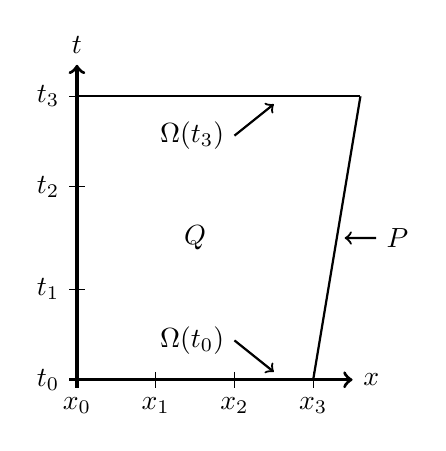
\begin{tikzpicture}[
    scale=1,
    axis/.style={very thick, ->},
    important line/.style={thick},
    every node/.style={color=black}
    ]
    %x-axis
    \draw[axis] (-0.1,0)  -- (3.5,0) node(xline)[right]{$x$};
    \foreach \x in {0,1,2,3}
    \draw (\x cm,0.1) -- (\x cm,-0.1) node[anchor=north] {$x_{\x}$};
    % t-axis
%    \draw[very thick] (0,-0.1) -- (0,1);
%    \draw[very thick] (0,1.3) -- (0,2.3);
    \draw[axis] (0,-0.1) -- (0,4) node(yline)[above]{$t$};
    \draw (0.1,0cm) -- (-0.1, 0cm) node[anchor=east] {$t_{0}$};
    \draw (0.1,1.15cm) -- (-0.1, 1.15cm) node[anchor=east] {$t_{1}$};
    \draw (0.1,2.45cm) -- (-0.1, 2.45cm) node[anchor=east] {$t_{2}$};
    \draw (0.1,3.6cm) -- (-0.1, 3.6cm) node[anchor=east] {$t_{3}$};
    % Lines
    \draw[important line] (3,0) coordinate (A)  -- (3.6,3.6) coordinate (B);
    \draw[important line] (0,3.6) coordinate (A)  -- (3.6,3.6) coordinate (B);
    \node (Q) at (1.5,1.8) {$Q$};
    \draw[thick,<-] (3.4,1.8cm) -- (3.8, 1.8) node[anchor=west] {$P$};
    \draw[thick,<-] (2.5,0.1cm) -- (2.0, 0.5) node[anchor=east] {$\Omega(t_0)$};
    \draw[thick,<-] (2.5,3.5cm) -- (2.0, 3.1) node[anchor=east] {$\Omega(t_3)$};
\end{tikzpicture}

    }
    \subcaptionbox{The time-discontinuous approach.\label{fig:dst}}{
    % CVPR 2023 Paper Template
% based on the CVPR template provided by Ming-Ming Cheng (https://github.com/MCG-NKU/CVPR_Template)
% modified and extended by Stefan Roth (stefan.roth@NOSPAMtu-darmstadt.de)

\documentclass[10pt,twocolumn,letterpaper]{article}
%%%%%%%%% PAPER TYPE  - PLEASE UPDATE FOR FINAL VERSION
%\usepackage[review]{cvpr}      % To produce the REVIEW version
\usepackage{cvpr}              % To produce the CAMERA-READY version
%\usepackage[pagenumbers]{cvpr} % To force page numbers, \eg for an arXiv version
\def\dg{\textcolor{red}}

% Include other packages here, before hyperref.
\usepackage{graphicx}
\usepackage{amsmath}
\usepackage{amssymb}
\usepackage{balance}
\usepackage{booktabs}
\usepackage{threeparttable}
\usepackage{multirow}
\usepackage{makecell}
\def\dg{\textcolor{red}}
\def\red{\textcolor{red}}
\def\lzm{\textcolor{blue}}

% It is strongly recommended to use hyperref, especially for the review version.
% hyperref with option pagebackref eases the reviewers' job.
% Please disable hyperref *only* if you encounter grave issues, \eg with the
% file validation for the camera-ready version.
%
% If you comment hyperref and then uncomment it, you should delete
% ReviewTempalte.aux before re-running LaTeX.
% (Or just hit 'q' on the first LaTeX run, let it finish, and you
%  should be clear).
\usepackage[pagebackref,breaklinks,colorlinks]{hyperref}
\hypersetup{
    colorlinks=true,
    linkcolor=red,
    citecolor=cyan,
    filecolor=magenta,      
    urlcolor=red,
    }
\usepackage[export]{adjustbox} % Vertical alignment
\usepackage{array,multirow}
\usepackage[accsupp]{axessibility}
% Support for easy cross-referencing
\usepackage[capitalize]{cleveref}
\crefname{section}{Section}{Sections.}
\Crefname{section}{Section}{Sections}
\Crefname{table}{Table}{Tables}
\crefname{table}{Table}{Table}
\Crefname{figure}{Figure}{Figures}
\crefname{figure}{Figure}{Figure}


%%%%%%%%% PAPER ID  - PLEASE UPDATE
\def\cvprPaperID{12597} % *** Enter the CVPR Paper ID here
\def\confName{CVPR}
\def\confYear{2023}


\begin{document}

%%%%%%%%% TITLE - PLEASE UPDATE
\title{Disentangling Writer and Character Styles for Handwriting Generation}

\author{Gang Dai$^{1}$\thanks{Authors contributed equally.}, Yifan Zhang$^{2*}$, Qingfeng Wang$^{1}$, Qing Du$^{1}$, 
Zhuliang Yu$^{1}$, \\ Zhuoman Liu$^{3}$, Shuangping Huang$^{1,4}$\thanks{Corresponding author} \\
$^{1}$South China University of Technology,
$^{2}$National University of Singapore, \\
$^{3}$The Hong Kong Polytechnic University,
$^{4}$Pazhou Laboratory \\
{\tt\small eedaigang@mail.scut.edu.cn}, {\tt\small yifan.zhang@u.nus.edu}, {\tt\small eehsp@scut.edu.cn}
}
\maketitle

%%%%%%%%% ABSTRACT
\begin{abstract}
   Training machines to synthesize diverse handwritings is an intriguing task. Recently, RNN-based methods have been proposed to generate stylized online Chinese characters. However, these methods mainly focus on capturing a person’s overall writing style, neglecting subtle style inconsistencies between characters written by the same person. For example, while a person's handwriting typically exhibits general uniformity (\eg, glyph slant and aspect ratios), there are still small style variations in finer details (\eg, stroke length and curvature) of characters. In light of this, we propose to disentangle the style representations at both writer and character levels from individual handwritings to synthesize realistic stylized online handwritten characters. Specifically, we present the style-disentangled Transformer (SDT), which employs two complementary contrastive objectives to extract the style commonalities of reference samples and capture the detailed style patterns of each sample, respectively. Extensive experiments on various language scripts demonstrate the effectiveness of SDT. Notably, our empirical findings reveal that the two learned style representations provide information at different frequency magnitudes, underscoring the importance of separate style extraction. Our source code is public at: \url{https://github.com/dailenson/SDT}.
\end{abstract}
\vspace{-0.1in}

%%%%%%%%% BODY TEXT
\section{Introduction}
\label{sec:intro}

% As the world's oldest writing system, Chinese characters are widely used in many Asian countries. Compared to Latin scripts, Chinese characters comprise an extremely large vocabulary (87,887 characters in GB18030-2022 charset) and have complex structures consisting of multiple strokes. Nowadays, the challenging and interesting Chinese character generation~\cite{zi2zi,gao2019artistic,liu2022xmp} has attracted intensive attention. For plausible handwriting synthesis, a promising strategy~\cite{zhang2017drawing} is to progressively generate online characters (\ie, the handwriting trajectory in a sequential format). As shown in \cref{fig:online}, online characters carry richer information (\eg, the order of writing) and thus have wide application scenarios (\eg, writing robot~\cite{yin2016synthesizing}).

As the oldest writing system, Chinese characters are widely used across Asian countries. When compared with Latin scripts, Chinese characters encompass an exceptionally vast lexicon (87,887 characters in GB18030-2022 charset) and have intricate structures composed of multiple strokes. Recently, the  intriguing task of generating Chinese characters has garnered significant attention~\cite{zi2zi,gao2019artistic,liu2022xmp}. A promising approach to synthesising realistic handwritings is  to progressively generate online characters (\ie, the handwriting trajectory in a sequential format)~\cite{zhang2017drawing}. As shown in \cref{fig:online}, online characters convey richer information  (\eg, the order of writing)  and thus pave the way for various applications, including writing robots~\cite{yin2016synthesizing}.

\begin{figure}[t]
\centering
\includegraphics[width=0.83\linewidth]{huakai_00.png}
\vspace{-0.05in}
\caption{Illustration of two online handwritten Chinese characters, with each color representing a stroke. The increasing numbers indicate the writing order from the start to the end.}
\label{fig:online}
\vspace{-0.2in}
\end{figure}

Our goal is to automatically generate online Chinese handwritings that not only correspond to specific textual content, but also emulate the calligraphic style of a given exemplar writer (\eg, glyph slant, shape, stroke length, and curvature). This task thus holds potential for a wide range of applications, such as font design and calligraphy education.  A popular solution~\cite{kang2020ganwriting} is to extract style information from the provided stylized samples and merge it with the content reference.  DeepImitator~\cite{zhao2020deep} concatenates the style vector obtained from a CNN encoder with a character embedding, which is then fed into the RNN decoder to generate stylized online characters. WriteLikeYou~\cite{tang2021write} adopts the large-margin softmax loss~\cite{wang2018cosface} to promote discriminative learning of style features. However, these methods mainly focus on the overall writing style, thus overlooking the detailed style inconsistencies (\eg, the highlighted regions in \cref{fig:style_inconsisitens}) between characters produced by the same writer.

\begin{figure}[t]\vspace{-0.1in}
\centering
\includegraphics[width=0.85\linewidth]{figure2.pdf}
\vspace{-0.1in}
\caption{Handwritten character samples from three unique writers, with each row containing characters by the same person. Despite sharing similar overall handwriting styles (\eg, glyph slant), subtle style differences (\eg, stroke length, location, and curvature) can still be observed among them.}
\label{fig:style_inconsisitens}
\vspace{-0.1in}
\end{figure}

The observations mentioned above inspire us to disentangle style representations at the writer and character levels from the stylized handwritings. However, accurately capturing these two styles is a challenging task. To address this, we propose a style-disentangled Transformer (SDT) equipped with a dual-head style encoder. Specifically, we employ the contrastive learning framework~\cite{hadsell2006dimensionality} to guide each head in concentrating on writer-wise and character-wise styles, respectively. For the overall writer-wise style, we treat characters from the same writer as positive instances, and characters from different writers as negatives. This  enables the encoder to learn the style commonalities among characters written by the same writer. Regarding the detailed character-wise style, we independently sample positive pairs within a character, and sample negative samples from other characters, as illustrated in \cref{fig:patch}. Aggregating positive views of a character encourages the encoder to focus on the intricate character style patterns.

In addition, we introduce a content encoder for SDT to learn a textual feature with a global context. The two style representations, along with the textual feature, are then fed into a decoder that progressively generates online characters. Given that the output characters are in sequential form, we employ Transformer~\cite{vaswani2017attention}, a powerful sequence modeling architecture, as our backbone.
 
To extend SDT for generating offline Chinese handwrittings (\ie, character images with stroke-width, \eg, Figures~\red{3-7} in Appendix), we further propose an offline-to-offline generation framework. We first use SDT to generate online characters with significant shape changes, and then decorate them with stroke width, ink-blot effects, \etc. This enables us to generate authentic offline handwritings. For more details, please refer to Appendix~\red{A.4}.


We summarize our contributions in three key aspects:
\begin{itemize}
  \item We are the first to disentangle two style representations (\ie, writer-wise and character-wise) for enhancing Chinese handwriting generation. Our findings show that the former focuses more on low-frequency information, while the latter captures higher frequencies.
  \item We introduce a novel online character generation method, \emph{\ie,} SDT. 
  Extensive experiments on handwriting datasets in Chinese, English, Japanese, and Indic scripts demonstrate its effectiveness and superiority.
  \item Building on the SDT, we further develop an offline-to-offline framework that can produce more plausible offline handwritten Chinese characters, as evidenced in Appendix \red{A.4}.
 
\end{itemize}

\begin{figure}[t]\vspace{-0.1in}
    \centering
    \includegraphics[width=0.79\linewidth]{figure3.pdf}
    \vspace{-0.1in}
    \caption{In this two-character example, we independently sample the positive pair, \ie, $o$ and $o^+$, within the first character, while the negative $o^-$ is sampled from another character. Our sampling strategy randomly selects a small subset of patches, following a uniform distribution.}
    \label{fig:patch}
    \vspace{-0.1in}
\end{figure}


\section{Related Work}

\noindent \textbf{Handwriting generation}.
Various style-content disentangling methods~\cite{aksan2018deepwriting, kang2020ganwriting,kotani2020generating,gan2021higan,luo2022slogan} have been proposed to generate handwritings with arbitrary styles. These methods assume that reference samples can be decomposed into style and content spaces. They disentangle calligraphic styles from reference samples and recombine them with specific textual content for controllable style synthesis. For instance,  DeepWriting~\cite{aksan2018deepwriting} adopts RNNs to extract the style vectors from online handwritings, and then combines them with character embeddings for synthesizing stylized online handwritings. However, it typically over-smooths the styles of distinct letters and loses key details, since its extracted style vectors are letter-independent~\cite{kotani2020generating}.

DSD~\cite{kotani2020generating} addresses the over-smooth problem by segmenting online handwritten words into isolated letters and encoding them into global and letter-specific style vectors, improving synthetic handwriting quality.  Compared with it, our method can explicitly capture more fine-grained details (\eg, stroke length, location and curvature), which are more difficult to obtain. Besides, these methods~\cite{aksan2018deepwriting,deepwritesyn,kotani2020generating} rely on  extra fine annotations to segment input cursive scripts, while our SDT need not. Recently, HWT~\cite{bhunia2021handwriting} uses a vanilla Transformer encoder for style pattern extraction. However, these methods~\cite{aksan2018deepwriting,kotani2020generating,bhunia2021handwriting,gan2021higan,kang2020ganwriting} rely on complex content references, such as recurrent embeddings and letter-wise filter maps. SLOGAN~\cite{luo2022slogan} addresses this issue by extracting textual contents from easily obtainable printed images, but  it struggles with generalizing to unseen handwriting styles  due to the fixed writer ID.  In contrast, our SDT effectively obtains content and style information, and thus can synthesize characters with arbitrary styles well. 

\begin{figure*}[t]
\vspace{-0.1in}
\centering
\includegraphics[width=0.75\linewidth]{figure4.pdf}
\caption{Overview of the proposed method. 
Our SDT consists of a dual-head style encoder, a content encoder and a Transformer decoder. The writer-wise and character-wise style representations extracted by style encoder and the learned content feature are fed into the Transformer decoder to progressively generate online handwritings.  We utilize the WriterNCE $\mathcal{L}_{wri}$ and GlyphNCE $\mathcal{L}_{gly}$ to guide the two heads for learning the corresponding styles. $\mathcal{L}_{pre}$ and $\mathcal{L}_{cls}$ denote the pen moving prediction and state classification loss, respectively.} 
\label{fig:overview}
\vspace{-0.1in}
\end{figure*}

Regarding handwritten Chinese characters, several attempts~\cite{kong2017handwritten, chang2018generating,huang2022AGTGAN} use GANs to generate Chinese handwriting images, but always result in characteristic artifacts. Drawing~\cite{zhang2017drawing} and FontRNN~\cite{tang2019fontrnn} adopt RNNs,  but they cannot flexibly control the handwriting styles. In addition, DeepImitator~\cite{zhao2020deep} and WriteLikeYou~\cite{tang2021write} propose style-controlled generation using style representations from offline images~\cite{zhao2020deep} or online trajectories\cite{tang2021write}. Unlike these methods~\cite{zhao2020deep, tang2021write} that only extract an overall writer style, our SDT captures both writer and character-level styles, significantly improving  the performance of handwriting imitation.

~

\noindent \textbf{Contrastive learning}.
Contrastive learning~\cite{hadsell2006dimensionality,zhang2021unleashing}  has been widely used in various fields~\cite{TianKI20,GaoYC21,ren2022learning,qiu2021source,zhangself,zhang2021deep}. Some image translation studies~\cite{park2020contrastive, han2021dual} use contrastive learning to enhance natural image generation quality, encouraging content preservation during transfer. Unlike these methods~\cite{park2020contrastive, han2021dual}, our SDT aligns independently sampled patches from the same input, aiming to improve style representations of handwritings.

\section{Method}
\noindent \textbf{Problem statement.}
We aim to synthesize stylized online handwritings with conditional content and style. Given a content image $I$ and a set of style images $X_s=\{x_s^i\}_{i=1}^K$, randomly sampled from a writer $w_s$, we aim to generate an online handwritten Chinese character $\hat{Y}_s$ that reflects the calligraphic style of $w_s$ and retains the textual content of~$I$. The key challenge lies in obtaining discriminative style representations from a limited number of stylized samples.

To address this task, inspired by our observations (cf.~\cref{fig:style_inconsisitens}) of the \textit{overall uniformity} (\ie, writer-wise style) and \textit{inconsistent details} (\ie, character-wise style), we propose to disentangle the style of exemplar writers into overall and detailed styles for enhancing handwriting imitation performance. To achieve this, we introduce a new style-disentangled Transformer (SDT) approach to decouple the two styles from individual handwritings. The overall scheme of SDT is presented below. 


\subsection{Overall Scheme}\label{overview} 
As shown in~\cref{fig:overview}, SDT consists of a dual-head style encoder, a content encoder, and a Transformer decoder. The style encoder (cf.~\cref{style_encoder}) is designed to learn the writer-wise and character-wise styles. It firstly extracts rich calligraphic style patterns from reference style examples $X_s$ via a sequential combination of a CNN and a Transformer encoder, followed by the writer and glyph heads to disentangle the writer-wise and character-wise styles from the extracted style patterns. To this end, we propose two contrastive objectives, WriterNCE $\mathcal{L}_{wri}$ and GlyphNCE $\mathcal{L}_{gly}$, to encourage the encoder to learn the two styles, respectively. Specifically,   $\mathcal{L}_{wri}$ maximizes the mutual information between character instances belonging to the same writer, while   $\mathcal{L}_{gly}$ associates the positive pair independently sampled from the same character. Guided by $\mathcal{L}_{wri}$ and $\mathcal{L}_{gly}$, the writer and glyph heads can acquire discriminative writer-wise and character-wise style features, respectively.

The content encoder uses a standard Resnet18~\cite{he2016deep} as the CNN backbone to learn the compact feature map $q_{map} \in \mathbb{R}^{h \times w \times c}$ from a content reference $I$, and feeds the flattened feature patches into a Transformer encoder to extract the textual content representation $q \in \mathbb{R}^{d \times c}$, where $d = h \times w$ and $c$ is the channel dimension. Benefiting from the strong capability of Transformer to capture long-range dependencies between feature patches, the content encoder expects an informative content feature $q$ with a global context. 

After the two encoders, a multi-layer Transformer decoder (cf. Section~\ref{Transformer_decoder}) is used to synthesize $\hat{Y}_s$ in an auto-regressive fashion, conditioned on the two style representations and the content feature. This decoder is supervised by the pen moving prediction loss $\mathcal{L}_{pre}$ and pen state classification loss $\mathcal{L}_{cls}$. 

To summarize, the overall training objective of SDT combines all four loss functions:
\begin{equation}\label{total}
\mathcal{L} = \mathcal{L}_{wri} + \mathcal{L}_{gly} + \mathcal{L}_{pre} + \lambda\mathcal{L}_{cls},
\end{equation}
where $\lambda$  serves as a trade-off factor. Each component of our SDT is detailed in the following \cref{style_encoder} and \cref{Transformer_decoder}.


%, where we omit the style $s$ of $X$ for the sake of simplicity

\subsection{Dual-head Style Encoder}\label{style_encoder}
As illustrated in~\cref{fig:style_inconsisitens}, there are two distinct styles in a person's handwriting: writer-wise and character-wise styles. We propose a dual-head style encoder to obtain the two style representations. As shown in~\cref{fig:overview}, the input $X=\{x^i\}_{i=1}^K$ is firstly encoded by  ResNet18 to obtain a sequence of feature maps $F_m = \{f_m^i\}_{i=1}^K \in\mathbb{R}^{K \times h \times w \times c}$. Next, we flatten the spatial dimension of each feature map to obtain feature sequences $F = \{f^i\}_{i=1}^K \in\mathbb{R}^{K \times d \times c}$. These feature sequences are then fed into a Transformer encoder to extract more informative feature sequences $Z = \{z^i\}_{i=1}^K \in\mathbb{R}^{K \times d \times c}$. 
Finally, we use the two heads, built on  self-attention~\cite{vaswani2017attention},  to further disentangle $Z$ into the writer-wise style representations $E = \{e^i\}_{i=1}^K \in\mathbb{R}^{K \times d \times c}$ via $\mathcal{L}_{wri}$ and the character-wise counterparts $G = \{g^i\}_{i=1}^K \in\mathbb{R}^{K \times d \times c}$ via $\mathcal{L}_{gly}$, respectively. We next detail the two contrastive learning objectives as follows.


\subsubsection{Writer-wise Contrastive Learning}\label{writer_style}
To explicitly encourage the writer head to learn the writer-wise style, we propose to learn a feature space where  the style features from the same writer are closer than those from different writers. The intuition is that one person's handwritings consistently exhibit similar style information, which can serve as a crucial clue for distinguishing writers. To this end,  we take characters written by the same person as positive pairs and those from different writers as negative samples, and develop a new WriterNCE loss for writer-wise style learning.



Specifically, let $j \in M=\{1, ..., N\} $ be the index of an  element within a mini-batch and let $A\left(j\right)=M \backslash \{j\}$ be other indices distinct from $j$, where $N$ is the batch size. Given a writer-wise style feature $e_j$ belonging to writer $w_j$ as the anchor, we denote its in-batch positive sample set as $P(j)=\{p \in A\left(j\right):w_p=w_j\}$ and its negative set as $A\left(j\right) \backslash P\left(j\right)$. The WriterNCE loss is formulated as follows: 
\begin{equation}\label{WriterNCE}
\mathcal{L}_{wri}\small{=}\frac{\small{-}1}{N}\sum_{j \in M}\frac{1}{	\left|P\left(j\right)\right|}\sum_{p \in P\left(j\right)}\log \frac{\exp{\left({{\rm sim}\left(e_j,e_p\right)}/\tau\right)}}{\sum_{a \in A\left(j\right)}\exp{\left({{\rm sim}\left(e_j,e_a\right)}/\tau\right)}},
\end{equation}
where ${\rm sim}\left(e_j,e_p\right)\small{=}f_1\left(e_j\right)^{\top}f_1(e_p)$, $\tau$ is a temperature parameter and $f_1\left(\cdot\right)$ is a multi-layer perceptron (MLP) that projects features to a $\ell_2$-normalized feature space where $\mathcal{L}_{wri}$ is applied.  

\subsubsection{Character-wise Contrastive Learning}\label{character_style}
Compared with the overall writer-wise style,   character-wise style differences often exist in the fine details of distinct characters, \eg, stroke length and curvature (cf. ~\cref{fig:patch}). Inspired by this, we aim to maximize the mutual information between diverse views of a character, thereby enforcing the glyph head to learn the  character-wise style. As strokes are distributed across arbitrary spatial locations in character images, we propose to capture  stroke details via contrastive learning, by randomly selecting a small subset of patches following a uniform distribution.  Specifically, we conduct sampling over the sequential patch tokens obtained from the glyph head.

Given character-wise style features $\{g_j\}_{j=1}^{B}\in\mathbb{R}^{B \times d \times c}$ extracted from $B$ characters, we sample a positive patch pair (\ie, $o \in \mathbb{R}^{n \times c}$ and $o^+ \in \mathbb{R}^{n \times c}$) from the same randomly selected $g$, and $B\small{-}1$ negative patches $\{o_j^-\}_{j=1}^{B\small{-1}}$ from the remaining $B\small{-}1$ style features. Here, the number of sampled patch tokens is $n=d\cdot\alpha$, where $\alpha$ is the sampling ratio. The GlyphNCE loss is formulated as:
\begin{equation}\label{GlyphNCE}
\mathcal{L}_{gly}\small{=-}\log \frac{\exp{\left({{\rm sim}\left(o,o^+\right)}/\tau\right)}}{\exp{\left({\rm sim}{\left(o,o^+\right)}/\tau\right)}\small{+}\sum_{j\small{=}1}^{B\small{-}1}\exp{\left({\rm sim}{\left(o,o_j^-\right)}/\tau\right)}},
\end{equation}
where ${\rm sim}\left(o,o^+\right)\small{=}f_2\left(o\right)^{\top}f_2(o^+)$, and $f_2(\cdot)$ is an MLP with the same structure as $f_1(\cdot)$.

\begin{figure}[t]
\centering  
\includegraphics[width=0.68\linewidth]{figure5.pdf}
    \caption{Illustration of the fusion of the style information in our Transformer decoder.  At each time step, the query vector is first encoded from the content feature $q$ and previous points $\{y_j\}_{j=1}^{t-1}$. Then, it successively attends to the writer-wise and character-wise style features (\ie, $E$ and $G$) for adaptively aggregating style information, which is finally decoded into the current-step output.}
    \label{fig:decoder}
    \vspace{-0.1in}
\end{figure}

\subsection{Transformer Decoder for Handwriting}\label{Transformer_decoder}
The goal of the Transformer decoder is to progressively generate realistic online characters, denoted as $\hat{Y}$,  based on the global content feature $q$ and the obtained style representations (\ie, $E = \{e^i\}_{i=1}^K$ and $G = \{g^i\}_{i=1}^K$). As each online character consists of numerous points (\ie, $\hat{Y}=\{{\hat{y}_j}\}_{j=1}^{L}$, with $L$ being the total number of points; see more details in Appendix \red{A.10}),  the decoder faces the challenge of effectively integrating content and style features to accurately depict all points of the character. To address this challenge,  we propose to fuse $q$, $E$ and $H$ within the multi-head attention layers of our Transformer decoder. As shown in \cref{fig:decoder},  $E$ and $H$ serve as the key/value vectors, while  $Q$ serves as the query vector that successively attends to $E$ and $G$ to aggregate style information.   
  
During training, at any decoding step $t$, we take $q$ as the initial point. As shown in~\cref{fig:decoder}, we apply self-attention 
to the point sequence, \ie the content context $\left[q, y_1, ..., y_{t-1}\right]$, to obtain the query vector $Q_t \in \mathbb{R}^c$. Here, the ground-truth points $\{{y_j}\}_{j=1}^{t-1}$ are used to accelerate model convergence in training~\cite{williams1989learning,tang2021write}. Subsequently, $Q_t$ attends to $E$ and $G$ over the subsequent decoding layers to adaptively aggregate style information, ultimately generating the output $O_t \in \mathbb{R}^{6R+3}$. The output with $6R+3$ logits is then used to generate the pen moving $\left(\Delta{\hat{u}_t}, \Delta{\hat{v}_t}\right)$ and  the pen state $\left( \hat{m}_t^1, \hat{m}_t^2, \hat{m}_t^3 \right)$. Specifically,  we use a Gaussian mixture model (GMM)~\cite{graves2013generating} with $R$ bivariate normal distributions to predict the pen moving, with each normal distribution containing 6 parameters. Moreover, we use the other $3$  logits  to generate the pen state. The training loss for supervising the decoder comprises two parts: the pen movement prediction loss  $\mathcal{L}_{pre}\left(\Delta{\hat{u}_t}, \Delta{\hat{v}_t}\right)$, and the pen state classification loss $\mathcal{L}{cls}\left(\hat{m}_t^1, \hat{m}_t^2, \hat{m}_t^3\right)$.  Please refer to Appendix \textcolor{red}{A.11} for more details of these losses.

The inference phase is different from the training phase, where the ground truth $y$ is not available at test time. Instead, we take the generated points$\{{\hat{y}_j}\}_{j=1}^{t-1}$ as the input of the step $t$, and combine them with $q$, $E$, and $G$ to predict the next point $\hat{y}_t$. Such a  process repeats until a pen-end state ($\hat{m}_{t-1}^3\small{=}1$) is received. %\dg{Notably, this generation process is not deterministic as each generated point $\hat{y}$ is sampled from the GMM. Thus, every time our method generates the same character, it exhibits minor variations in appearance, which bears a strong resemblance to the process of human writing.}


\section{Experiments}
\subsection{Chinese handwriting generation}

\noindent \textbf{Dataset.}
To evaluate  SDT in generating Chinese handwritings, we use CASIA-OLHWDB~(1.0-1.2)~\cite{liu2011casia} for model training and ICDAR-2013 competition database~\cite{yin2013icdar} for testing. The training set consists of about 3.7 million online Chinese handwritten characters produced by 1,020 writers, while the test set contains 60 writers, with each contributing 3,755 most frequently used characters set of GB2312-80. Following~\cite{ICLRSKETCH}, we use the Ramer–Douglas–Peucker algorithm~\cite{douglas1973algorithms} with a parameter of $\epsilon=2$ to remove redundant points of characters, leading to an average sequence length of 50. Following ~\cite{zhao2020deep}, we render offline style references using coordinate points of online characters, and each style sample is randomly sampled from the target-writer handwritings during inference, as shown in~\cref{fig:overview}. For content images, we use the popular average Chinese font~\cite{jiang2019scfont}.

\begin{figure*}[t]
    \centering
    \includegraphics[width=0.82\linewidth]{figure6.pdf}
    \vspace{-0.1in}
    \caption{Comparisons with the state-of-the-art methods for online Chinese handwriting generation. The red and blue boxes highlight failures of style imitation and structure preservation, respectively. WriteLi. indicates the WriteLikeYou-v2. The green boxes highlight comparisons between the fine details of targets and generated characters.}
    \label{fig:sota_method}
    \vspace{-0.1in}
\end{figure*}


\noindent \textbf{Evaluation metrics}\label{QEM}.
We use Dynamic Time Warping (DTW)~\cite{berndt1994using,chen2022complex}, an elastic matching technique for aligning the given two sequences, to calculate the distance between the generated and real characters. Moreover, we use Content Score ~\cite{zhao2020deep} to measure the structure correctness of generated characters, and adopt Style Score~\cite{tang2021write} to quantify the style similarity between the generated and real handwritings.
We also conduct user preference studies to quantify the subjective quality of the output characters. More details are provided in Appendix~\red{A.1.1}.


\noindent\textbf{Implementation details}. We set the number of the style reference to $K=15$, and resize the reference style and content images to $64 \times 64$. Moreover, each Transformer encoder contains 2 self-attention layers, while the Transformer decoder has 4 layers for obtaining style representations (2 for writer-wise and 2 for character-wise).  Following the origginal Transformer~\cite{vaswani2017attention}, each Transformer layer contains the multi-head attention with $c= 512$ dimensional states and 8 attention heads.  Contrary to HWT~\cite{bhunia2021handwriting}, where $F$ is concatenated before the Transformer encoder, we process each feature sequence $f \in F$ individually.  Moreover, we apply sinusoidal positional encoding~\cite{vaswani2017attention} to  input tokens before feeding them to the Transformer encoder and decoder. For training, we first pre-train the content encoder with 138k iterations (batch size of 256) for character classification on training samples and then train the whole model with 148k iterations (batch size of 128), on a single RTX3090 GPU. The optimizer is Adam~\cite{kingma2015adam}, with a learning rate of 0.0002 and gradient clipping of 5.0.  The sampling ratio $\alpha$ is determined through a search over ${0.25, 0.5, 0.75, 1.00}$, and 0.25 is chosen. Following ~\cite{tang2021write}, we set $\lambda=2$. Further implementation details are provided in Appendix~\red{A.1.2}.

% \begin{table}
% 	\caption{Comparisons with state-of-the-art methods on Chinese dataset.}
%     \begin{center}
%     \scalebox{0.8}{
%     \begin{threeparttable} 
% 	\begin{tabular}{lcccc}\toprule
%         Method  &  \makecell[c]{Style \\ Score $\uparrow$}  & \makecell[c]{Content \\ Score $\uparrow$} & DTW $\downarrow$ & \makecell[c]{User \\ Prefer. $\left(\%\right)$ $\uparrow$} \\ \midrule 
%         Drawing~\cite{zhang2017drawing} & 38.75 &78.15 & 1.1813 & 4.73  \\
%         FontRNN~\cite{tang2019fontrnn} & 46.14 & 92.18 & 1.0448 & 9.93 \\
%         DeepImitator~\cite{zhao2020deep} & 51.69 &90.92 & 1.0622 & 10.27  \\
%         WriteLikeYou~\cite{tang2021write} & 73.07 &93.89 & 0.9832 & 17.20  \\
%         SDT(Ours) & \textbf{94.50} & \textbf{97.04} & \textbf{0.8789} & \textbf{57.87}  \\
%         \bottomrule
% 	\end{tabular} 
%     \end{threeparttable}
%     }
%     \end{center}
%     \label{tab:com_sota} 
% \end{table} 

\noindent \textbf{Compared methods}. We compare our proposed SDT with state-of-the-art online Chinese character generation methods, \ie Drawing~\cite{zhang2017drawing}, FontRNN~\cite{tang2019fontrnn}, DeepImitator~\cite{zhao2020deep}, and WriteLikeYou~\cite{tang2021write}. To ensure a fair comparison, we re-implement Drawing and FontRNN by adding the style branch of DeepImitator~\cite{zhao2020deep}, enabling them to achieve arbitrary stylized character generation. To adapt WriteLikeYou~\cite{tang2021write} to handle images, we update its encoder to create two new variants: WriteLikeYou-v1 (\ie, CNN encoder~\cite{zhao2020deep}) and WriteLikeYou-v2 (\ie, the same CNN-Transformer encoder as our SDT), based on the released official code\footnote{\url{https://github.com/ShusenTang/WriteLikeYou}}. More  details are available in Appendix \red{A.1.3}.

\begin{figure*}[t]
    \centering
    \includegraphics[width=0.9\linewidth]{figure7.pdf} 
    \vspace{-0.1in}
    \caption{Spectrum analysis of two style representations. We provide frequency magnitude visualizations belonging to $7$ writers, where the top row shows the writer-wise style while the bottom represents the character-wise one. Each spectrum map is averaged over 100 character samples written by the same person. The brighter the color, the larger the magnitude. A pixel farther from the center means a higher frequency~\cite{pan2022hilo}. We find that the writer-wise style representations capture more low-frequency information, while character-wise style representations capture more high-frequency information.}
    \vspace{-0.1in}
    \label{fig:fft}
\end{figure*}

\begin{table}
	\caption{Comparisons with  state-of-the-art methods on  Chinese dataset. See more results of WriteLikeYou~\cite{tang2021write} in Appendix \red{A.6.}}
    \vspace{-0.2in}
    \begin{center}
    \scalebox{0.8}{
    \begin{threeparttable} 
	\begin{tabular}{lcccc}\toprule
        Method  &  \makecell[c]{Style \\ Score $\uparrow$}  & \makecell[c]{Content \\ Score $\uparrow$} & DTW $\downarrow$ & \makecell[c]{User \\ Prefer. $\left(\%\right)$ $\uparrow$} \\ \midrule 
        Drawing~\cite{zhang2017drawing} & 35.83 &78.15 & 1.1813 & 3.53  \\
        FontRNN~\cite{tang2019fontrnn} & 46.14 & 92.18 & 1.0448 & 7.07 \\
        DeepImitator~\cite{zhao2020deep} & 50.67 &90.92 & 1.0622 & 7.99  \\
        WriteLikeYou-v1~\cite{tang2021write} & 71.09 &93.89 & 0.9832 & 11.67  \\
        WriteLikeYou-v2~\cite{tang2021write} & 72.37 &96.44 & 0.9289 & 13.07 \\
        SDT(Ours) & \textbf{94.50} & \textbf{97.04} & \textbf{0.8789} & \textbf{56.67}  \\
        \bottomrule
	\end{tabular} 
    \end{threeparttable}
    }
    \end{center}
    \label{tab:com_sota} 
    \vspace{-0.1in}
\end{table}

\noindent \textbf{Quantitative comparison}. Quantitative results are  in~\cref{tab:com_sota}, revealing that SDT outperforms other methods across all evaluation metrics. Notably, SDT surpasses the second-best method by a significant 22.13\% margin in Style Score, demonstrating the proposed method's exceptional style imitation performance.

\noindent \textbf{Qualitative comparison}. 
We visualize the generated samples of each method in~\cref{fig:sota_method}, which intuitively explains the significant superiority of SDT in the user preference study. In~\cref{fig:sota_method}, Drawing~\cite{zhang2017drawing} generates the least satisfactory results, often producing unreadable characters. FontRNN~\cite{tang2019fontrnn} and DeepImitator~\cite{zhao2020deep} occasionally synthesize unpleasant stroke paddings, and WriteLikeYou~\cite{tang2021write}  struggles with generating complex characters regarding style mimicry. In contrast, our method yields higher-quality results, particularly in recovering fine character details.
 
\subsection{Analysis}\label{abl}

In this section, we assess the impact of the two learned style features and that of the style inputs. We also analyze the effect of the sampling ratio $\alpha$, and discuss the combination strategies in the Transformer decoder in Appendix \red{A.5}. Besides, we discuss failure cases in Appendix \red{A.7}.
 
\noindent \textbf{Quantitative evaluation of two style representations.} We ablate  the effects of the two extracted style representations in~\cref{two_style}. The  findings include: (1) Both style representations enhance the quality of generated outcomes in all evaluation metrics, particularly in terms of Style Score, improving by 4.79\% and 5.86\%, respectively. (2) Combining the two style features further boosts model performance across all evaluation metrics, suggesting that the extracted styles are complementary. Moreover, the order in which the two style features are input into the Transformer decoder has no significant impact on  Style Score (93.72\% vs. 94.50\%).

\begingroup
\begingroup
\begin{table}[t!]
    \centering
    \caption{Ablation study. Here, we further use FID to measure the distance between generated and real samples for each writer separately, and finally average them.} 
 
    \label{two_style}
    \renewcommand\arraystretch{2.15}{
    \scalebox{0.6}{
    \begin{tabular}{cc |ccc |ccc}
     %\toprule
     \hline
     writer-wise & character-wise & \multicolumn{3}{c|}{Generated Samples} & Style Score$\uparrow$ & FID$\downarrow$  & DTW$\downarrow$  \\
        %\midrule
        \hline
         &  &    \includegraphics[scale=0.35,valign=c]{1_qin_base1.png} &
        \includegraphics[scale=0.35,valign=c]{9_jie_base2.png} &
        \includegraphics[scale=0.35,valign=c]{23_chao_resize.png}  & 85.52  & 27.75& 0.8941  \\
        \checkmark &  & \includegraphics[scale=0.35,valign=c]{1_qin_global.png} &
        \includegraphics[scale=0.35,valign=c]{9_jie_global.png} &
        \includegraphics[scale=0.35,valign=c]{23_chao_global.png} & 91.38 & 26.38&0.8841 \\
        & \checkmark &\includegraphics[scale=0.35,valign=c]{1_qin_local.png} &
        \includegraphics[scale=0.35,valign=c]{9_jie_local.png} &
        \includegraphics[scale=0.35,valign=c]{23_chao_local.png} & 90.31&26.89&0.8803
        \\
        \checkmark & \checkmark & 
        
        \includegraphics[scale=0.35,valign=c]{1_qin_twobranch.png} &
        \includegraphics[scale=0.35,valign=c]{9_jie_twobranch.png} &
        \includegraphics[scale=0.35,valign=c]{23_chao_twobranch.png} & 94.50&25.46&0.8789 \\
        \hline
        %\cmidrule{1-8}
        \multicolumn{2}{c|}{Ground Truth} &\includegraphics[scale=0.35,valign=c]{1_qin_gt.png} &
        \includegraphics[scale=0.35,valign=c]{9_jie_gt.png} &
        \includegraphics[scale=0.35,valign=c]{23_chao_gt.png}  &&&  \\
        %\bottomrule
        \hline
    \end{tabular}}
    }
    \vspace{-0.1in}
\end{table}
\endgroup

%  \begin{table}
% \caption{Effect of two style representations. $G\small{-}E$ denotes the Transformer decoder first receives character-wise style features and then accepts writer-wise ones (and vice versa).}
% \vspace{-0.1in}
% \centering
%     \scalebox{0.83}{
%     \begin{threeparttable} 
% 	\begin{tabular}{cccccc}\toprule
%         character-wise & writer-wise & $G\small{-}E$ & $E\small{-}G$  & Style Score$\uparrow$ \\ \midrule 
%           &  & & &  85.52  \\
%          $\checkmark$ & & &  & 90.31  \\
%           & $\checkmark$ & & & 91.38  \\
%          $\checkmark$ & $\checkmark$ &$\checkmark$ &  & 93.72  \\
%      $\checkmark$ & $\checkmark$&  &  $\checkmark$ & 94.50 \\
%         \bottomrule
% 	\end{tabular} 
%     \end{threeparttable}}
%     \label{two_style}
% \end{table}
 
\noindent \textbf{Qualitative comparison between two style representations.}
To further analyze the differences between the two styles, we resize the output patch tokens representing the two styles to feature maps, respectively, and visualize their frequency magnitudes in~\cref{fig:fft}. We find that character-wise style features capture more high-frequency information, whereas writer-wise features mainly focus on low-frequency information. According to~\cite{cooley1969fast}, the high-frequency information in an image usually captures fine details while the low frequencies contain the overall part of objects. This finding supports our motivation that the writer head helps to imitate the overall style (\eg, glyph slant), while the glyph head captures the detailed style (\eg, stroke curvature), as shown in~\cref{two_style}. 


% \begin{table}[t]
% 	\caption{Quantitative evaluations of our SDT and competitors on Japanese dataset.}
% 	\vspace{-0.25in}
% 	\label{tab:Janpanese}
%     \begin{center}
%     \scalebox{0.8}{
%     \begin{threeparttable} 
% 	\begin{tabular}{lccc}\toprule
%     Methods & Style Score $\uparrow$ & Content Score$\uparrow$ & DTW $\downarrow$\\ \midrule 
%       Drawing~\cite{zhang2017drawing}  & 20.67 & 50.74 & 1.4657  \\
%       DeepImitator~\cite{zhao2020deep}  & 25.80 & 53.20 & 1.2564  \\
%        WriteLikeYou-v2~\cite{tang2021write}  & 32.88 & 85.61 & 1.2066 \\
%        SDT(Ours)  & \textbf{41.85} & \textbf{91.31} & \textbf{1.1289} \\
%         \bottomrule
% 	\end{tabular} 
%     \end{threeparttable}}
%     \end{center}
%     \vspace{-0.3in}
% \end{table}



 \begin{figure}[t] 
    \centering
\includegraphics[width=0.82\linewidth]{dtw_matrix_60_1_00.png}
    \vspace{-0.1in}
    \captionof{figure}{The heat map of the DTW matrix. The dark diagonal indicates that the generated characters still own a higher similarity even using different $X_s$ belonging to the same writer.}
    \vspace{-0.1in}
    \label{fig:dtw} 
\end{figure}





\begin{table}[t]
	\caption{Quantitative evaluations of our SDT and competitors on Japanese, Indic, and English datasets.}
    \vspace{-0.1in}
	\label{tab:foreign}
    \begin{center}
    \scalebox{0.85}{
    \begin{threeparttable} 
	\begin{tabular}{cccc}\toprule
    Datasets & Methods & Content Score$\uparrow$ & DTW $\downarrow$\\ \midrule 
     \multirow{4}{*}{Japanese} & Drawing~\cite{zhang2017drawing} & 50.74 & 1.4657  \\
     & DeepImitator~\cite{zhao2020deep} & 53.20 & 1.2564  \\
     &  WriteLikeYou-v2~\cite{tang2021write}   & 85.61 & 1.2066 \\
     &  SDT(Ours)  & \textbf{91.31} & \textbf{1.1289} \\
     \midrule 
     \multirow{4}{*}{Indic} & Drawing~\cite{zhang2017drawing} & 2.34 & 9.8230  \\
     & DeepImitator~\cite{zhao2020deep} & 4.13 & 6.7421  \\
     &  WriteLikeYou-v2~\cite{tang2021write}   & 13.19 & 4.5130 \\
     &  SDT(Ours)  & \textbf{97.22} & \textbf{0.7075} \\
     \midrule 
     \multirow{4}{*}{English} & Drawing~\cite{zhang2017drawing} & 79.14 & 1.8519  \\
     & DeepImitator~\cite{zhao2020deep} & 76.53 & 1.6460  \\
     &  WriteLikeYou-v2~\cite{tang2021write}   & 84.41 & 1.6215 \\
     &  SDT(Ours)  & \textbf{85.52} & \textbf{1.6048} \\
        \bottomrule
	\end{tabular} 
    \vspace{-0.1in}
    \end{threeparttable}}
    \end{center}
\end{table}



\begin{figure*}[t]
    \centering
    \includegraphics[width=0.9\linewidth]{figure9.pdf} 
    \caption{Comparisons with the competitors for online handwriting generation on various scripts. WriteLi. indicates WriteLikeYou-v2.}
    \label{fig:foreign_com} 
\end{figure*}




\noindent \textbf{Effect of using different style inputs.} As mentioned in ~\cite{tang2021write}, given different style inputs $X_s$ belonging to the same writer $w_s$, the imitation model may generate inconsistent characters. To evaluate the effect of different style inputs, we conduct two independent experiments using different $X_s$ based on the same model. Following~\cite{tang2021write}, we use the model to generate 200 characters for each writer in the test set. We then calculate the DTW distance between corresponding characters individually and average them according to the writer index (see Appendix \red{A.1.4} for more details) to get a DTW square matrix. The resulting DTW square matrix is visualized in Figure~\ref{fig:dtw}. The dark diagonal in Figure~\ref{fig:dtw} suggests that the generated characters maintain a high degree of similarity even when using different $X_s$ belonging to the same writer, demonstrating that our SDT can generate consistent results from various style inputs.

% \begin{table}
% 	\caption{Quantitative evaluations of our SDT and competitors on Indic datatset.}
% 	\vspace{-0.1in}
% 	\centering
% 	\scalebox{0.85}{
%     \begin{threeparttable} 
% 	\begin{tabular}{lcc}\toprule
%      Methods & Content Score$\uparrow$ & DTW $\downarrow$\\ \midrule 
%       Drawing~\cite{zhang2017drawing}  & 2.34 & 9.8230  \\
%       DeepImitator~\cite{zhao2020deep}  & 4.13 & 6.7421 \\
%       WriteLikeYou-v2~\cite{tang2021write}  & 13.19 & 4.5130 \\
%       SDT(Ours)  & \textbf{97.22} & \textbf{0.7075} \\ \bottomrule
% 	\end{tabular}
%     \end{threeparttable}}
%     \label{tab:Indic}
%     \vspace{-0.15in}
% \end{table}

\subsection{Applications to Other Languages}

\noindent \textbf{Japanese handwriting generation}.
For the Japanese handwriting generation task, we conduct experiments on TUAT HANDS~\cite{matsumoto2001collection} database~(see more details in Appendix \red{A.1.5}) to evaluate the effectiveness of our method. \cref{fig:foreign_com} (a) and \cref{tab:foreign} verify the effectiveness of SDT for Japanese handwriting generation. Specifically, from \cref{tab:foreign}, we observe that our SDT outperforms all compared methods in terms of two quantitative metrics, indicating that  SDT performs well in multiple languages. Furthermore, we provide additional evaluation metrics in Appendix \textcolor{red}{A.8}.



\noindent \textbf{Indic handwriting generation}.
We evaluate our method on the Indic handwriting generation task based on the Tamil\footnote{\url{http://lipitk.sourceforge.net/datasets/tamilchardata.htm}} dataset.  It is worth noting that Indic handwriting generation presents a more significant challenge, as Indic characters contain more trajectory points than Chinese, Japanese, and English scripts (i.e., 88 vs. 68, 50, 30 on average; see Appendix \textcolor{red}{A.1.5} for more dataset information). We compare our method with other approaches on the official test set in terms of Content Score and Dynamic Time Warping (DTW). As shown in Table~\ref{tab:foreign},  we find that our SDT significantly outperforms the second-best method in terms of the two quantitative metrics, achieving an 84.03\% higher Content Score and a 3.8055 lower DTW. This indicates that our SDT can handle handwritten characters with a large number of points (averaging 88) and ensure the quality of synthetic samples, as illustrated in Figure~\ref{fig:foreign_com} (b). The potential advantages of our SDT are: (1) The improved style representations extracted by our SDT prevent the collapse of generated characters. (2) Our Transformer decoder facilitates long-distance dependence between trajectory points. We provide more experimental analysis in Appendix \textcolor{red}{A.9}.

 ~

\noindent \textbf{English handwriting generation}.
To evaluate our method in generating  English handwritings,  we collect all of the English samples from the symbol part of CASIA-OLHWDB(1.0-1.2)~\cite{liu2011casia} and ICDAR-2013 competition database~\cite{yin2013icdar} (see more details in Appendix \red{A.1.5}). Similarly, we use Content Score and DTW as evaluation metrics. As shown in Figure~\ref{fig:foreign_com} (c), we find that all methods achieve sound and comparable performance. One reason for this is that the English script contains fewer character classes and a smaller number of trajectory points (averaging 30), making their imitation easier compared to other scripts. Nevertheless, our SDT still outperforms other methods by a small margin in terms of both Content Score and DTW, as shown in Table~\ref{tab:foreign}. Moreover, we observe that corresponding uppercase and lowercase letters sometimes exhibit subtle inter-class differences (\eg, O vs. o), which leads our SDT to achieve a relatively low Content Score.



\section{Conclusion}
In this paper,  we have proposed a novel method, named style-disentangled Transformer (SDT), to synthesize realistic and diverse online handwritings.
SDT enhances imitation performance by disentangling the  writer-wise and  character-wise style representations from  individual handwriting samples. For the writer-wise style, we group characters from the same writer and separate those from different writers, promoting SDT's ability to learn uniformity in individual handwritings.  For the character-wise style, we  maximize the mutual information between the distinct views of a character. Moreover, we extend SDT and introduce an offline-to-offline framework for improving the generation quality of offline Chinese handwritings. Promising results on various language scripts verify the effectiveness of our SDT. Although primarily designed for handwriting generation, SDT still holds the potential for extension to other generative tasks, such as font generation.

\paragraph{Acknowledgments}
This research is partially supported by NSFC (Grant No.62176093, 61673182), Key Realm R\&D Program of Guangzhou (No.202206030001), Guangdong Basic and Applied Basic Research Foundation (No.2021A1515012282) and Guangdong Provincial Key Laboratory of Human Digital Twin (2022B1212010004).


\clearpage
%%%%%%%%% REFERENCES
{ 
\small
\balance
\bibliographystyle{ieee_fullname}
\bibliography{egbib}
}

\end{document}

    }

    \caption{Definition of the computational domain(s) in the space-time approach for deforming domain problems.}
    \label{fig:parametricProblemComputationalDomain}
\end{figure}
\bigskip
\par
To be able to eventually demonstrate the presented approach, we consider a specific example of fluid flow equations here. In particular, we make use of the \textit{Stokes equations}, which can be used to model a variety of fluid flow of low Reynolds number, for example.
Based on the conservation of mass and momentum, the Stokes equations provide statements for the, in this case parametric, \textit{velocity} and \textit{pressure} fields of the fluid, which are referred to as $\vel(\x,t;\paramVec)$ and $\p(\x,t;\paramVec)$, respectively. Here, $\paramVec$ denotes the \textit{parameter vector} collecting parameter values to vary either material properties or boundary conditions.
Note that we will drop the arguments of $\vel$ and $\p$ for the sake of notation in the following. Nevertheless, dependencies on $\paramVec$ will be stressed if necessary.
\par
The resulting \gls{bvp} in the space-time setting reads as follows:
\begin{align}
        \dv{\vel(\paramVec)} &= 0 &&\text{ in } \domainSpaceTime,
        \\
        \density \lp \dd{\vel(\paramVec)}{t} - \bdf \rp - \dv{\cstressParam{\vel}{\p}} &= \vek{0} &&\text{ in } \domainSpaceTime,
        \\
        \vel(\paramVec) &= \velDirichlet(\paramVec) &&\text{ on } \boundarySpaceTimeDirichlet,
        \\
        \cstressParam{\vel}{\p}\cdot \vek{n} &= \tractionNeumann(\paramVec) &&\text{ on } \boundarySpaceTimeNeumann,
        \\
        \vel(\x,0;\paramVec) &= \vel_0(\paramVec) &&\text{ in } \domainSpace(t_0).
\end{align}
Here, $\density$ is the fluid \textit{density}, $\bdf$ is a \textit{body force}, while $\velDirichlet(\paramVec)$, $\vel_0(\paramVec)$, and $\tractionNeumann(\paramVec)$ are the parameter-dependent prescribed velocity values and a \textit{traction vector}, respectively. 
Moreover, we consider parametric material properties through the fluid \textit{viscosity} $\visc(\paramVec)$ that is included in the \textit{Cauchy stress tensor} given by
\begin{align}
    \cstressParam{\vel}{\p} = - \p\lp\paramVec\rp \mat{I} + 2 \visc\lp\paramVec\rp \ros{\vel\lp\paramVec\rp},
\end{align}
where
$
    \ros{\vel} = \frac{1}{2} ( \vek{\nabla} \vel + \vek{\nabla} \vel^T )
$
is the \textit{rate-of-strain tensor}.
In the following, we will consider fluid materials whose viscous properties cannot be appropriately described by a Newtonian model. Examples for such non-Newtonian fluids are plastics melt or blood. 
To account for shear-thinning effects of the fluid, we use the Carreau-Yasuda model \cite{Carreau1972, Yasuda1981, Bird1987} for the viscosity, which depends on the shear rate 
\begin{align}
\shearrate(\vel; \paramVec) = \sqrt{2 \ros{\vel(\paramVec)} : \ros{\vel(\paramVec)}}.   
\end{align}
To stress the dependency on the velocity field, we from now on write $\visc(\vel; \paramVec)$ given by
\begin{align}
       % \visc(\vel; \paramVec) &= \frac{A}{\left(1+B\shearrate\right)^{C}},
        %\\
        \visc(\vel; \paramVec)
        &= 
        \visc_{\infty} 
        + \left( \visc_0 - \visc_{\infty} \right) \left[ 1 + \left( \lambda \shearrate \right)^a \right]^{\frac{n-1}{a}},
    \label{eq:viscosityModel}
\end{align}
with zero-shear-rate viscosity $\visc_0$, infinite-shear-rate viscosity $\visc_{\infty}$, characteristic time $\lambda$, power-law index $n$, and a dimensionless parameter $a$ describing the transition region between the zero-shear-rate viscosity and the power-law regions.
In addition to the indirect parameter dependency of the viscosity through the parametric velocity field, we also take into account potential fluctuations in the model parameters. This is motivated by the fact that these model parameters can only be determined through a regression-based approach using measurement data associated with uncertainties. 
\bigskip\par
Since the \gls{fem} will be used later to construct the \gls{fom} in \Cref{sec:fullOrderModel}, which in turn will serve as the basis for the \gls{rom} presented in \Cref{sec:reducedOrderModel}, it is worthwhile to state the \textit{weak formulation} of the problem here. We will assume that appropriate trial and weighting spaces for the velocity and the pressure field in the space-time domain $\domainSpaceTime$ are given. For the velocity, the trial and weighting spaces are denoted as $\trialSpaceVelocity(\domainSpaceTime)$ and $\weightingSpaceVelocity(\domainSpaceTime)$, respectively. For the pressure, the trial space is also the weighting space and they are referred to as $\trialSpacePressure(\domainSpaceTime)$. The resulting weak formulation of the parametric problem defined in the space-time domain $\domainSpaceTime$ reads:
\bigskip\par\noindent
\textit{Find }$\lp \trialVelocityParam, \trialPressureParam \rp 
\in 
\trialSpaceVelocity\lp\domainSpaceTime\rp 
\times 
\trialSpacePressure\lp\domainSpaceTime\rp $\textit{, such that }$\forall \lp \weightVelocity, \weightPressure \rp 
\in 
\weightingSpaceVelocity\lp\domainSpaceTime\rp 
\times 
\weightingSpacePressure\lp\domainSpaceTime\rp $\textit{:}
\begin{align}
    &
    \intDomainSpaceTime
    {
        \weightVelocity \cdot \density 
        \lp
            \dd{\trialVelocityParam}{t} - \bdf
        \rp
    }
    -
    \intDomainSpaceTime
    {
        \trialPressureParam \lp \dv{\weightVelocity}\rp
    }
    \nonumber
    \\
    +
    &
    \intDomainSpaceTime
    {
        \ros{\weightVelocity} : 2 \visc\lp\vel,\paramVec\rp \ros{\trialVelocity}
    }
    +
    \intDomainSpaceTime
    {
        \weightPressure \lp \dv{\trialVelocityParam}\rp
    }
    =
    \intBoundarySpaceTimeNeumann
    {
        \weightVelocity \cdot \tractionNeumann\lp\paramVec\rp
    }
    .
    \label{eq:navierStokesWeakExtended}
\end{align}
To simplify notation, the following short forms will be used in the remainder of this work:
\begin{align*}
    \begin{aligned}[t]
        \ddt{\trialVelocity}\lp\paramVec\rp 
        &= 
        \dd{\trialVelocityParam}{t},
        \\
        \bilinearFormPressureParam{\trialVelocity}{\weightPressure}{\paramVec}_{\domainSpaceTime}  
        &=     
        \intDomainSpaceTime
        {
            \weightPressure \lp \dv{\trialVelocityParam}\rp
        },
        \\
        \lp \weightVelocity, \bdf \rp_{\domainSpaceTime} 
        &=
        \intDomainSpaceTime
        {
           \density \weightVelocity \cdot \bdf
        },
    \end{aligned}
    \qquad
    \begin{aligned}[t]
        \lp \weightVelocity, \ddt{\trialVelocity}; \paramVec \rp_{\domainSpaceTime} 
        &= 
        \intDomainSpaceTime
        {
           \density \weightVelocity \cdot \ddt{\trialVelocity}\lp\paramVec\rp
        },
        \\
        \bilinearFormViscousStressParam{\weightVelocity}{\trialVelocity}{\trialVelocityHom}{\paramVec}_{\domainSpaceTime}  
        &=     
        \intDomainSpaceTime
        {
            \ros{\weightVelocity} : 2 \visc\lp \trialVelocityHom,\paramVec\rp \ros{\trialVelocity}
        },
        \\
        \lp \weightVelocity, \tractionNeumann; \paramVec \rp_{\boundarySpaceTimeNeumann}
        &=     
        \intBoundarySpaceTimeNeumann
        {
            \weightVelocity \cdot \tractionNeumann\lp\paramVec\rp
        }
        .
    \end{aligned}
\end{align*}
In this notation, \Cref{eq:navierStokesWeakExtended} can be stated as
\begin{align}
    \lp \weightVelocity, \ddt{\trialVelocity}; \paramVec \rp_{\domainSpaceTime} 
    - \bilinearFormPressureParam
    {\weightVelocity}
    {\trialPressure}{\paramVec}_{\domainSpaceTime} 
    + \bilinearFormViscousStressParam
    {\weightVelocity}
    {\trialVelocity}
    {\vel}
    {\paramVec}_{\domainSpaceTime}
    +\bilinearFormPressureParam
    {\trialVelocity}
    {\weightPressure}{\paramVec}_{\domainSpaceTime}
    =
    \lp \weightVelocity, \bdf \rp_{\domainSpaceTime}  
    +\lp \weightVelocity, \tractionNeumann; \paramVec \rp_{\boundarySpaceTimeNeumann}
    .
\end{align}
\section{Full-Order Model for Fluid Flow in Deforming Domains}
\label{sec:fullOrderModel}
In this section, we will derive the \gls{fom} which results from applying the \gls{fem} to the parametric problem introduced beforehand. In particular, this model will be capable of simulating transient problems in deforming domains. To that end, \Cref{subsec:methodologicalBackgroundFOM}  will first contain a brief outline of existing techniques that address deforming domain problems in this context. Subsequently, we present the space-time \gls{fem} used in this work in \Cref{subsec:discreteFormulationFOM}.

\subsection{Methodological Background for Deforming Domains in the Full-Order Model}
\label{subsec:methodologicalBackgroundFOM}
In the following, we will roughly outline existing approaches for deforming domain problems, i.e., problems including moving boundaries or internal interfaces, without claiming completeness. First, one can make a division into interface capturing and interface tracking methods \cite{Elgeti2016}. Well-known examples for interface capturing methods, which employ an implicit description of domain boundaries or interfaces on a background mesh, are the level-set method \cite{Osher1988,Chang1996} or the volume-of-fluid method \cite{Hirt1981}. In contrast, interface tracking methods are based on boundary-conforming meshes. Thus, an update procedure that adapts the computational mesh according to the deforming domain is needed.
\par
There exist a vast number of strategies, ranging from global remeshing to elaborate methods specifically designed for certain applications or types of deformation. As examples for connectivity-preserving methods that update nodal coordinates, one can mention \gls{pde}-based methods like the \gls{emum} \cite{Tezduyar1992}, spring-based methods \cite{Batina1990} or techniques using radial basis functions \cite{DeBoer2007}. Further methods extend these strategies by a subsequent mesh optimization, e.g., through edge swapping or vertex smoothing operations \cite{Alauzet2013,Wang2015a}. Moreover, specialized mesh update methods use algebraic operations to control the mesh evolution for a-priori known boundary deformations~\cite{Helmig2019, Hinz2020}. Furthermore, local remeshing strategies limit the cost of maintaining a high quality boundary-conforming mesh under large deformations~\cite{Behr1999,Behr2001,Behr2003}. Broadening the scope of these methods, parts of the mesh can be activated and deactivated~\cite{Key2018} and topology changes of the computational domain can be handled elegantly~\cite{Gonzalez2023}.
\par
As an alternative, one can also follow weak domain coupling strategies to account for the moving boundary or interface by using composite grids and introducing additional conditions on the solution field. Examples are the Chimera method \cite{Steger1983, Benek1986, Steger1987} or sliding interface approaches \cite{Bazilevs2008, Takizawa2015, Helmig2020}. It is also worthwhile to mention the immersed boundary method \cite{Peskin1972}, where simulations are always performed on a cartesian background grid.
\par
Deforming domain problems are inherently transient and their solution requires a form of time discretization. Common approaches include time-stepping methods which separate spatial and temporal discretization and space-time methods which apply a combined discretization to the space-time domain. Time stepping schemes, e.g., the generalized $\alpha$-method~\cite{Chung1993}, require an arbitrary Lagrangian–Eulerian (ALE) formulation for moving-domain simulations~\cite{Hughes1981, Donea2004}, while the space-time formulation directly accounts for the (spatial) mesh deformation~\cite{Tezduyar1992a, Tezduyar1992b}.
\par
If the movement is known during mesh generation --- typically this means before the simulation start --- the time-continuous space-time approach allows to incorporate complex deformations of the spatial domain in a boundary-conforming space-time mesh. Even topology changes can be included as shown in finite volume and finite element simulations~\cite{Rendall2012, Danwitz2019}. For two-dimensional problems, standard mesh generation tools can be used to construct the three-dimensional space-time mesh. For three-dimensional problems, more sophisticated mesh generation and adaptation techniques are required. The common approach to generate an unstructured four-dimensional mesh is based on the extrusion of a tetrahedral mesh followed by a subdivision of the prismatic elements into pentatopes (4-simplices). The subdivision can either be achieved with an element-wise Delaunay triangulation~\cite{Behr2008} or with a predefined decomposition which requires a consistently numbered tetrahedral mesh~\cite{Karabelas2019}. Further techniques enable refinement and anisotropic adaptation of four-dimensional meshes~\cite{Neumueller2011, Wang2015a, Caplan2020}.  Four-dimensional meshes with complex deformations and topology changes of the three-dimensional spatial domain can be obtained with an elastic mesh update following extrusion based pentatope mesh generation~\cite{Danwitz2021}. Please, note that the additional effort for the space-time mesh generation completely replaces the special treatment of a deforming domain problem during the simulation. Nevertheless, our boundary-conforming space-time mesh approach is limited to 4D geometries that can be obtained by extrusion of a 3D geometry and a subsequent elastic deformation. Generating meshes for general 4D geometries of engineering scale is -- to the best of our knowledge -- an open research problem.
\subsection{Discrete Formulation for the Full-Order Model}
\label{subsec:discreteFormulationFOM}
Next, we will derive the \gls{fom}, which will be based on the \gls{fem}. Thus, we introduce corresponding finite dimensional subspaces for the trial and weighting spaces introduced in \Cref{sec:parametricFormulation}. Let $\trialSpaceVelocityDiscrete(\domainSpaceTime)$ and $\weightingSpaceVelocityDiscrete(\domainSpaceTime)$ be the finite dimensional subspaces of $\trialSpaceVelocity(\domainSpaceTime)$ and $\weightingSpaceVelocity(\domainSpaceTime)$, respectively. Furthermore, $\trialSpacePressureDiscrete(\domainSpaceTime)$ is the finite dimensional subspace of $\trialSpacePressure(\domainSpaceTime)$. We  stick to the \textit{\gls{csst}} approach, i.e., the computational mesh will be composed of simplex elements filling the entire space-time domain $\domainSpaceTime$. Furthermore, we use first-order polynomials as shape functions $\basisFunctionVelocityFOM{i}$ and $\basisFunctionPressureFOM{i}$ for velocity and pressure, respectively.
\par
To handle (parametric) Dirichlet boundary conditions, we introduce a \textit{velocity lifting function} $\liftingVelocityDiscrete(\paramVec)$ such that the \textit{discrete velocity trial function} is given as
\begin{align}
    \trialVelocityDiscrete(\paramVec) = \trialVelocityHomDiscrete(\paramVec) + \liftingVelocityDiscrete(\paramVec),
\end{align}
with the homogeneous portion $\trialVelocityHomDiscrete(\paramVec)$ and $\liftingVelocityDiscrete(\paramVec)\lvert_{\boundarySpaceTimeDirichlet}=\velDirichlet(\paramVec)$.
Note that additional lifting functions may be used to separate parameter-dependent and independent portions of the Dirichlet boundary conditions.
For the sake of notation, however, we only consider the case of a single lifting function here.
%Note that $\liftingVelocityDiscrete$ can be split into parameter-dependent and independent parts . 
Consequently, it holds that $\trialVelocityDiscrete \in \trialSpaceVelocityDiscrete(\domainSpaceTime)$ and $ \trialVelocityHomDiscrete \in \weightingSpaceVelocityDiscrete(\domainSpaceTime)$. Moreover, the \textit{discrete pressure trial function} is denoted as $\trialPressureDiscreteParam \in \trialSpacePressureDiscrete(\domainSpaceTime)$
\iffalse
The ansatz for the velocity and the pressure is given as:
\begin{align}
    \trialVelocityHomDiscrete 
    =
    \sum_{B=1}^{\nBasisVelocityFOM}
    \coeffVelocityFOM{B}
    \basisFunctionVelocityFOM{B}
    ,
    &&\trialPressureDiscrete
    =
    \sum_{B=1}^{\nBasisPressureFOM}
    \coeffPressureFOM{B}
    \basisFunctionPressureFOM{B},
\end{align}
with corresponding basis functions $\basisFunctionVelocityFOM{B}$, $\basisFunctionPressureFOM{B}$ and coefficients $\coeffVelocityFOM{B}$, $\coeffPressureFOM{B}$. The number of basis functions for each field is denoted as $\nBasisVelocityFOM$ or $\nBasisPressureFOM$.
\bigskip\par
Up to now, we have followed the standard Galerkin approach just as before. In doing so, the numerical treatment of these equations reveals two kinds of difficulties, which have to be opposed with appropriate stabilization techniques (see e.g. \cite{Donea2003} and references therein). First, the incompressibility constraint leads to a problem of saddle-point character. As a consequence, the choice of element interpolation functions, e.g., the order of the polynomials, becomes critical. More specifically, the spaces for velocity and pressure have to be chosen in a way in which the famous \gls{lbb} or \textit{inf-sup} condition is satisfied. Inappropriate choices may lead to pressure instabilities. Note that this phenomenon is independent of the presence of convective effects and, therefore, independent of the Reynolds number.
As has been mentioned before, we restrict ourselves to first order polynomial, i.e., linear elements, for both the velocity and pressure. However, for this choice the \gls{lbb} condition is not fulfilled.
The second difficulty arises when the non-linear convective effects are dominant, leading to spurious spatial oscillations.
\par
\fi
\par
We apply the \gls{gls} stabilization technique \cite{Hughes1987,Hughes1989,Mittal1992,Shakib1991}, which adds a least-squares form of the residual within each element to the original variational formulation of the problem. In the \gls{csst} formulation, this will apply to space-time elements denoted by $\domainSpaceTime^e$.
\iffalse
\begin{itemize}
    \item stabilization needed for
    \begin{enumerate}
        \item \gls{lbb} condition
        \item temporal term works like advection term in space-time setting
    \end{enumerate}
\end{itemize}
\fi
\bigskip\par
Following the description, e.g., from \cite{Behr1994,Franca1992}, the resulting space-time Galerkin formulation including the additional stabilization terms reads:
%\todo[inline]{Add contribution of \texttt{dtInGls on}}
\bigskip\par\noindent
\textit{Find }$\lp \trialVelocityHomDiscreteParam, \trialPressureDiscreteParam \rp 
\in 
\weightingSpaceVelocityDiscrete\lp\domainSpaceTime\rp
\times 
\trialSpacePressureDiscrete\lp\domainSpaceTime\rp$\textit{, such that }$\forall \lp \weightVelocityDiscrete, \weightPressureDiscrete \rp 
\in
\weightingSpaceVelocityDiscrete\lp\domainSpaceTime\rp 
\times 
\weightingSpacePressureDiscrete\lp\domainSpaceTime\rp$\textit{:}
\begin{align}
    \lp \weightVelocityDiscrete, \ddt{\trialVelocityHomDiscrete}; \paramVec \rp_{\domainSpaceTime} 
    - \bilinearFormPressureParam
    {\weightVelocityDiscrete}
    {\trialPressureDiscrete}{\paramVec}_{\domainSpaceTime} 
    + \bilinearFormViscousStressParam
    {\weightVelocityDiscrete}
    {\trialVelocityHomDiscrete}{\trialVelocityDiscrete}{\paramVec}_{\domainSpaceTime}
    +\bilinearFormPressureParam
    {\trialVelocityHomDiscrete}
    {\weightPressureDiscrete}{\paramVec}_{\domainSpaceTime}&
    \nonumber
    \\
    +\bilinearFormStabMomStokesTemporalParam
    {\weightPressureDiscrete}
    {\trialVelocityDiscrete}
    {\trialPressureDiscrete}
    {\trialVelocityDiscrete}
    {\paramVec}_{\domainSpaceTime}&
    \nonumber
    \\
    =
    \lp \weightVelocityDiscrete, \bdf \rp_{\domainSpaceTime}  
    +\lp \weightVelocityDiscrete, \tractionNeumann; \paramVec \rp_{\boundarySpaceTimeNeumann}
    -\lp \weightVelocityDiscrete, \ddt{\liftingVelocityDiscrete}; \paramVec \rp_{\domainSpaceTime} 
    -\bilinearFormViscousStressParam
    {\weightVelocityDiscrete}
    {\liftingVelocityDiscrete}{\trialVelocityDiscrete}{\paramVec}_{\domainSpaceTime}
    -\bilinearFormPressureParam
    {\liftingVelocityDiscrete}
    {\weightPressureDiscrete}{\paramVec}_{\domainSpaceTime}&
    ,
    \label{eq:navierStokesGalerkinStabilizedST}
\end{align}
with
\iffalse
\begin{align}
    &\bilinearFormStabMomStokesTemporal
    {\weightPressureDiscrete}
    {\trialVelocityDiscrete}
    {\trialPressureDiscrete}
    _{\domainSpaceTime} 
    =
    \sum_{e} \intElementSpaceTime{\tMom \frac{1}{\rho}
    \lp
        -\gr{\weightPressureDiscrete} 
        \rp
        \cdot 
        \lp
        \rho \ddt{\trialVelocityDiscrete}
        - \gr{\trialPressureDiscrete}
    \rp}.
\end{align}
\fi
\begin{align}
\bilinearFormStabMomStokesTemporalParam
    {\weightPressureDiscrete}
    {\trialVelocityDiscrete}
    {\trialPressureDiscrete}
    {\trialVelocityDiscrete}
    {\paramVec}
    _{\domainSpaceTime} 
    =
    s^{\trialVelocityHom}\lp\weightPressureDiscrete,\trialVelocityHomDiscrete;\trialVelocityDiscrete,\paramVec\rp_{\domainSpaceTime}
    +
    s^{\vek{l}}\lp\weightPressureDiscrete,\liftingVelocityDiscrete;\trialVelocityDiscrete,\paramVec\rp_{\domainSpaceTime}
    +
    s^{\trialPressure}\lp\weightPressureDiscrete,
    \trialPressureDiscrete;\trialVelocityDiscrete,\paramVec\rp_{\domainSpaceTime},
\end{align}
and
\begin{align}
    s^{\trialVelocityHom}
    \lp
    \weightPressureDiscrete,
    \trialVelocityHomDiscrete;
    \trialVelocityDiscrete,
    \paramVec
    \rp_{\domainSpaceTime}
    &=
    \sum_{e} \intElementSpaceTime{\tMom \frac{1}{\rho}
    \lp
    -\gr{\weightPressureDiscrete} 
    \rp
    \cdot 
    \lp
    \rho \ddt{\trialVelocityHomDiscrete}\lp\paramVec\rp
    \rp
    },
    \\
    s^{\vek{l}}
    \lp
    \weightPressureDiscrete,
    \liftingVelocityDiscrete;
    \trialVelocityDiscrete,
    \paramVec
    \rp_{\domainSpaceTime}
    &=
    \sum_{e} \intElementSpaceTime{\tMom \frac{1}{\rho}
    \lp
    -\gr{\weightPressureDiscrete} 
    \rp
    \cdot 
    \lp
    \rho \ddt{\liftingVelocityDiscrete}\lp\paramVec\rp
    \rp
    },
    \\
    s^{\trialPressure}
    \lp
    \weightPressureDiscrete,
    \trialPressureDiscrete;
    \trialVelocityDiscrete,
    \paramVec
    \rp_{\domainSpaceTime}
    &=
    \sum_{e} \intElementSpaceTime{\tMom \frac{1}{\rho}
    \gr{\weightPressureDiscrete} 
    \cdot 
    \gr{\trialPressureDiscreteParam} 
    }.
\end{align}
\par
The stabilization parameter $\tMom$ is chosen as presented in \cite{Pauli2016a}. Although the formulation in detail is not of great importance for this work, note that it depends both on the parametric velocity $\trialVelocityDiscrete(\paramVec)$ and the parametric viscosity $\visc(\trialVelocityDiscrete, \paramVec)$ in a non-linear way. Furthermore, the second-order derivatives of the velocity weighting and trial functions, which appear in the original formulation of the momentum stabilization, are omitted due to the first-order linear basis functions in use.
\bigskip\par
As a foundation for the description of the \gls{rom} in the following section, we present next the \textit{algebraic formulation} of the problem. The vectors of coefficients are denoted as $\velocityDOFVector \in \mathbb{R}^{\nBasisVelocityFOM}$ and $\pressureDOFVector\in \mathbb{R}^{\nBasisPressureFOM}$ for the homogeneous velocity $\trialVelocityHomDiscrete$ and pressure field $\trialPressureDiscrete$, respectively. Here, $\nBasisVelocityFOM$ and $\nBasisPressureFOM$ stand for the number of \glspl{dof} in the \gls{fom}. The solution can then be computed by solving the following non-linear system for $\velocityDOFVectorParam$ and $\pressureDOFVectorParam$:
\begin{align}
    \lb
    \begin{array}{cc}
        \matrixTemporal + \matrixViscousStressParam         &  -\matrixPressureTrans 
        \\
        \matrixPressure + \matrixStabMomStokesTemporalParam & \matrixStabMomStokesParam
    \end{array}
    \rb
    \lb
    \begin{array}{c}
        \velocityDOFVectorParam\\
        \pressureDOFVectorParam
    \end{array}
    \rb
    =
    \lb
    \begin{array}{c}
         \vectorRHSTemporal + \vectorRHSVelocity + \vectorRHSVelocityNonlinearParam\\
         \vectorRHSPressure + \vectorRHSStabMomStokesTemporalParam
    \end{array}
    \rb&
    ,
    \label{eq:algebraicSystemFOM}
\end{align}
where the \gls{lhs} matrices for $i,j = 1, \dots, \nBasisVelocityFOM $ and for $k,l = 1, \dots, \nBasisPressureFOM $ are given as
\begin{align*}
    \begin{aligned}[t]
        \matrixTemporal &= \lb \matrixTemporalSymbol_{i,j} \rb, 
        \text{ with } 
        \matrixTemporalSymbol_{i,j} 
        = 
        \lp \basisFunctionVelocityFOM{i}, \dd{\basisFunctionVelocityFOM{j}}{t} \rp_{\domainSpaceTime},
        \\
        \matrixPressure &= \lb\matrixPressureSymbol_{k,j}\rb,
        \text{ with }
        \matrixPressureSymbol_{k,j} 
        = 
        \bilinearFormPressure
        {\basisFunctionVelocityFOM{j}}
        {\basisFunctionPressureFOM{k}}_{\domainSpaceTime},
        \\
        \matrixStabMomStokes &= \lb \matrixStabMomStokesSymbol_{k,l}\rb,
        \text{ with }
        \matrixStabMomStokesSymbol_{k,l}
        = 
        s^{\trialPressure}
        \lp
        \basisFunctionPressureFOM{k},
        \basisFunctionPressureFOM{l};
        \trialVelocityDiscrete,
        \paramVec
        \rp_{\domainSpaceTime},
    \end{aligned}
    \quad
    \begin{aligned}[t]
        \matrixViscousStress &= \lb A_{i,j}\rb,
        \text{ with } 
        \matrixViscousStressSymbol_{i,j} 
        = 
        \bilinearFormViscousStressParam
        {\basisFunctionVelocityFOM{i}}
        {\basisFunctionVelocityFOM{j}}
        {\trialVelocityDiscrete}
        {\paramVec},    
        \\
        \matrixStabMomStokesTemporal &= \lb \matrixStabMomStokesTemporalSymbol_{k,j}\rb,
        \text{ with }
        \matrixStabMomStokesTemporalSymbol_{k,j}
        = 
        s^{\trialVelocityHom}
        \lp
        \basisFunctionPressureFOM{k},
        \basisFunctionVelocityFOM{j};
        \trialVelocityDiscrete,
        \paramVec
        \rp_{\domainSpaceTime},
    \end{aligned}
\end{align*}
and the \gls{rhs} vectors read
\begin{align*}
    \begin{aligned}[t]
        \vectorRHSTemporal &= \{ \vectorRHSTemporalSymbol_i\}, 
        \text{ with }
        \vectorRHSTemporalSymbol_i 
        =
        - \lp \basisFunctionVelocityFOM{i}, \ddt{\liftingVelocityDiscrete};\paramVec \rp_{\domainSpaceTime}, 
        \\
        \vectorRHSVelocityNonlinear &= \{\vectorRHSVelocityNonlinearSymbol_i\},
        \text{ with }
        \vectorRHSVelocityNonlinearSymbol_i = 
        - \bilinearFormViscousStressParam
        {\basisFunctionVelocityFOM{i}}
        {\liftingVelocityDiscrete}
        {\trialVelocityDiscrete}
        {\paramVec},
        \\
        \vectorRHSStabMomStokesTemporal &= \{ \vectorRHSStabMomStokesTemporalSymbol_{k}\}
        \text{, with }
        \vectorRHSStabMomStokesTemporalSymbol_{k}
        = 
        -s^{\vek{l}}
        \lp
        \basisFunctionPressureFOM{k},
        \liftingVelocityDiscrete;
        \trialVelocityDiscrete,
        \paramVec
        \rp_{\domainSpaceTime}.
    \end{aligned}
    \quad
    \begin{aligned}[t]
        \vectorRHSVelocity &= \{\vectorRHSVelocitySymbol_i\},
        \text{ with }
        \vectorRHSVelocitySymbol_i
        =
        \bilinearFormNeumannSpaceTimeParam
        {\basisFunctionVelocityFOM{i}}
        {\nval}
        {\paramVec},
        \\
        \vectorRHSPressure &= \{G_k\},
        \text{ with }
        G_k
        =
        -\bilinearFormPressureParam
        {\liftingVelocityDiscrete}
        {\basisFunctionPressureFOM{k}}
        {\paramVec}_{\domainSpaceTime},
    \end{aligned} 
\end{align*}
For convenience, the dimensions of the matrices and vectors are summarized in \Cref{tab:dimensionsFOM}.
\begin{table}
    \centering
    \begin{tabular}{lclc}
        \toprule
        \acrshort{lhs} Matrices & Dimensions & \acrshort{rhs} Vectors & Dimensions\\
        \midrule
        $\matrixTemporal$, $\matrixViscousStress$ & $\mathbb{R}^{\nBasisVelocityFOM \times \nBasisVelocityFOM}$ & $\vectorRHSTemporal$, $\vectorRHSVelocity$, $\vectorRHSVelocityNonlinear$ & $\mathbb{R}^{\nBasisVelocityFOM}$  \\
        $\matrixPressure$, $\matrixStabMomStokesTemporal$ & $\mathbb{R}^{\nBasisPressureFOM \times \nBasisVelocityFOM}$ & $\vectorRHSPressure$, $\vectorRHSStabMomStokesTemporal$ & $\mathbb{R}^{\nBasisPressureFOM}$  \\
        $\matrixStabMomStokes$ & $\mathbb{R}^{\nBasisPressureFOM \times \nBasisPressureFOM}$ \\
        \bottomrule
    \end{tabular}
    \caption{Dimensions of \acrshort{lhs} matrices and \acrshort{rhs} vectors for the \acrshort{fom}.}
    \label{tab:dimensionsFOM}
\end{table}

\section{Reduced-Order Model for Fluid Flow in Deforming Domains}
\label{sec:reducedOrderModel}
Now that the \gls{fom} has been defined, we can turn to the \gls{mor}. We will start with a description of the underlying ideas of \gls{mor} in \Cref{subsec:methodologicalBackgroundROM} before the \gls{rom} is eventually constructed via \gls{pod} with subsequent projection in \Cref{subsec:discreteFormulationROM}.

\subsection{Methodological Background for the Reduced-Order Model}
\label{subsec:methodologicalBackgroundROM}
In the context of \gls{mor} for numerical schemes, one can distinguish between \textit{interpolation}- and \textit{projection}-based approaches \cite{Manzoni2012}. Methods of the former type try to directly capture input-output relations on the basis of data that comes from numerical simulations or measurements. The latter project the underlying governing equations onto a reduced space that has been constructed before. The class of projection-based methods further entails \textit{certified \gls{rb}} methods \cite{Hesthaven2015} or \textit{\gls{pod}-projection} methods \cite{Chinesta2011,Hesthaven2015,Manzoni2012}. It is also worthwhile to mention the \textit{\gls{pgd}}~\cite{Chinesta2011} here.
\par
In view of the fact that we would like to focus on the class of unsteady problems in deforming domains, one can note that the application of \gls{mor} techniques requires some thorough treatment in this case.
\par
To account for the unsteady character of the problem in the reduction process, there exist two alternative ways of handling time \cite{Glas2017}. The first one follows the classical time-stepping approach, leading to so-called greedy or \gls{pod}-greedy methods, which have been applied to linear as well as to nonlinear problems \cite{Drohmann2012, Fick2018, Grepl2005a, Grepl2012, Haasdonk2008, Haasdonk2013, Sleeman2022}. The second one is rather based on space-time formulations for which reduction techniques for steady problems have been extended appropriately \cite{Urban2012, Urban2013, Tamma2018, Yano2014a, Yano2014b}. This perspective has been used to tackle, e.g., time-dependent optimal control problems \cite{Strazzullo2020, Strazzullo2022}. In addition, a space-time \gls{rom} for sub-intervals of the total simulation time has been presented in \cite{Fritzen2018a}. In distinction to the former methods, we will apply the \gls{pod}-projection approach to the time-continuous space-time formulation stated beforehand.
\par
The construction of a \gls{rom} for deforming domain problems is usually quite involved and requires some careful treatment of the deformations applied to the computational mesh \cite{Anttonen2001,Forti2014}. This is due to the fact that the \gls{fem} function spaces are inherently linked with the geometry of the underlying grid. A strategy based on a mapping functional to relate the time-dependent solution in one- and two-dimensional deforming domains to fixed reference domains has been presented in \cite{Izadi2013}. Furthermore, temporally-local eigenfunctions have been used for \gls{mor} in \cite{Narasingam2017}. 
To this respect, the \gls{csst} approach (cf. \Cref{subsec:discreteFormulationFOM}) offers an appealing but straightforward alternative, since all deformations --- as long as they are prescribed or known a-priori --- are already integrated in the computational mesh and, thereby, considered in the original function spaces. Also, it is worthwhile to note that this approach even works in the presence of spatial topology changes and for two- and three-dimensional spatial domains without any further adaptions.

\subsection{Discrete Formulation for the Reduced-Order Model}
\label{subsec:discreteFormulationROM}
Before we can construct an efficient \gls{rom} whose complexity is independent of the \gls{fom}, we will have to address the non-linearity appearing in our problem through the viscosity model as well as through the formulation of the stabilization parameter.  
For this purpose, we make use of the \gls{eim} \cite{Barrault2004, Grepl2007} here and introduce the following approximations for the viscosity and the stabilization parameter:
\begin{align*}
    \visc\left(\trialVelocityDiscrete, \paramVec\right) 
    \approx
    \sum_{q=1}^{Q_{\visc}} c_q^{\visc}\lp\trialVelocityDiscrete, \paramVec\rp h_q^{\visc}\lp\x\rp,
    &&
    \tMom%\left(\trialVelocityDiscrete, \paramVec\right) 
    \approx
    \sum_{q=1}^{Q_{\tau}} c_q^{\tau}\lp\trialVelocityDiscrete, \paramVec\rp  h_q^{\tau}\lp\x\rp
    .
\end{align*}
Note that each of the $Q_{\star}$ terms consists of parameter-dependent coefficients $c_q^{\star}\lp\trialVelocity, \paramVec\rp$ and parameter-independent basis functions $h_q^{\star}\lp\x\rp$, where $\star\in\{\visc,\tau\}$.
Consequently, the viscous term is replaced by
\begin{align}
    \bilinearFormViscousStressParam{\weightVelocityDiscrete}{\trialVelocityHomDiscrete}{\trialVelocityDiscrete}{\paramVec}_{\domainSpaceTime}
    \approx
    \sum_{q=1}^{Q_{\visc}} c_q^{\visc}\lp\trialVelocityDiscrete, \paramVec\rp 
    a_q\lp\weightVelocityDiscrete, \trialVelocityHomDiscrete\rp_{\domainSpaceTime},
\end{align}
with
\begin{align}
    a_q\lp\weightVelocityDiscrete, \trialVelocityHomDiscrete\rp_{\domainSpaceTime}
    =
    \intDomainSpaceTime
    {
        \ros{\weightVelocityDiscrete} : 2 h_q^{\visc}\lp\x\rp \ros{\trialVelocityHomDiscrete}
    }.
\end{align}
Moreover, the stabilization term $s^{\trialVelocityHom}$ is approximated via
\begin{align}
    s^{\trialVelocityHom}\lp\weightPressureDiscrete,\trialVelocityHomDiscrete;\trialVelocityDiscrete, \paramVec\rp_{\domainSpaceTime}
    \approx
    \sum_{q=1}^{Q_{\tau}} c_q^{\tau}\left(\trialVelocityDiscrete, \paramVec\right)
    s^{\trialVelocityHom}_q\lp\weightPressureDiscrete,\trialVelocityHomDiscrete\rp_{\domainSpaceTime},
\end{align}
where
\begin{align}
    s^{\trialVelocityHom}_q\lp\weightPressureDiscrete,\trialVelocityHomDiscrete\rp_{\domainSpaceTime}
    =
    \sum_{e} \intElementSpaceTime{\basisFunctionEIM{q}{}^{\tau}\lp\x\rp \frac{1}{\rho}
    \lp
    -\gr{\weightPressureDiscrete}
    \rp
    \cdot
    \lp
    \rho \ddt{\trialVelocityHomDiscrete}
    \rp
    }.
\end{align}
Analogously, the remaining stabilization terms 
$s^{\vek{l}}
    (\weightPressureDiscrete,
    \liftingVelocityDiscrete;
    \trialVelocityDiscrete,
    \paramVec)_{\domainSpaceTime}$ 
    and
$s^{\trialPressure}(
    \weightPressureDiscrete,
    \trialPressureDiscrete;
    \trialVelocityDiscrete
    \paramVec)_{\domainSpaceTime}$ 
can be approximated using parameter-independent terms
$s_q^{\vek{l}}
    (\weightPressureDiscrete,
    \liftingVelocityDiscrete)_{\domainSpaceTime}$
    and
$s_q^{\trialPressure}(
    \weightPressureDiscrete,
    \trialPressureDiscrete)_{\domainSpaceTime}$,
respectively. As a consequence, all the matrices and vectors in the algebraic system of the \gls{fom} relying on these forms, i.e., $\matrixViscousStress$, $\matrixStabMomStokesTemporal$, $\matrixStabMomStokes$, $\vectorRHSVelocityNonlinear$, and $\vectorRHSStabMomStokesTemporal$ are replaced by approximations using $\matrixViscousStress^q$, $\matrixStabMomStokesTemporal^q$, $\matrixStabMomStokes^q$, $\vectorRHSVelocityNonlinear^q$, and $\vectorRHSStabMomStokesTemporal^q$ corresponding to the respective terms above. For example, this means $\matrixViscousStress^q = \lb \matrixViscousStressSymbol^q_{i,j}\rb,
        \text{ with } 
        \matrixViscousStressSymbol^q_{i,j} 
        = 
        a_q\lp\basisFunctionVelocityFOM{i},\basisFunctionVelocityFOM{j}\rp_{\domainSpaceTime}$.
\bigskip\par
To perform the projection step later, a basis spanning the reduced spaces is needed. To that end, we apply the \gls{pod} using the method of snapshots~\cite{Sirovich1987}, i.e., solutions of the \gls{fom}. In particular, this is done individually for the homogeneous velocity $\trialVelocityHomDiscrete$ and the pressure $\trialPressureDiscrete$ leading to the \textit{reduced finite-dimensional function spaces} $\weightingSpaceVelocityReduced \subset \weightingSpaceVelocityDiscrete$ and $\weightingSpacePressureReduced \subset \trialSpacePressureDiscrete$.
As a result of the \gls{pod}, we obtain $\nBasisVelocityHomROM$ and $\nBasisPressureROM$ basis functions for the reduced representation $(\trialVelocityHomReduced,\trialPressureReduced)$ of the homogeneous velocity and pressure field, respectively. To account for the Dirichlet boundary conditions, the basis for $\weightingSpaceVelocityReduced$ is augmented with the lifting function(s) $\liftingVelocityDiscrete$ yielding the reduced space $\trialSpaceVelocityReduced \subset \trialSpaceVelocityDiscrete$ for the reduced velocity $\trialVelocityReduced$. Therefore, we use $\nBasisVelocityROM \ge \nBasisVelocityHomROM$ to denote the number of basis functions for $\trialVelocityReduced$. We sort the basis functions in descending order of significance --- indicated by the magnitude of the corresponding eigenvalues --- while the lifting functions are always leading to ensure that the Dirichlet boundary conditions are met, even if we only use a subset of these basis functions.
\par
For all basis functions, we collect the coefficients with respect to the \gls{fom} function spaces in the so-called \textit{basis function matrices} $\basisFunctionMatrixVelocity\in\mathbb{R}^{\nBasisVelocityFOM \times \nBasisVelocityROM}$ and $\basisFunctionMatrixPressure\in\mathbb{R}^{\nBasisPressureFOM \times \nBasisPressureROM}$. These matrices are multiplied with those from the algebraic system of the \gls{fom} given in \Cref{eq:algebraicSystemFOM}, which yields the projection of the corresponding operators onto the reduced space. Thus, one can formulate the algebraic system for the vectors of unknowns $\velocityDOFVectorReduced\in\mathbb{R}^{\nBasisVelocityROM}$ and $\pressureDOFVectorReduced\in\mathbb{R}^{\nBasisPressureROM}$, where $\nBasisVelocityROM$ and $\nBasisPressureROM$ are the number of unknowns of the \gls{rom}. Key assumption for an effective reduction is that it holds that $\nBasisROM = \nBasisVelocityROM + \nBasisPressureROM \ll \nBasisFOM = \nBasisVelocityFOM + \nBasisPressureFOM$. The system finally reads:
\begin{align}
    \lb
    \begin{array}{cc}
        \matrixTemporalReduced + \matrixViscousStressReducedParam
         & -\matrixPressureReducedTrans
        \\
        \matrixPressureReduced + \matrixStabMomStokesTemporalReducedParam& \matrixStabMomStokesReducedParam
    \end{array}
    \rb
    \lb
    \begin{array}{c}
        \velocityDOFVectorReducedParam\\
        \pressureDOFVectorReducedParam
    \end{array}
    \rb&
    \nonumber
    \\
    =
    \lb
    \begin{array}{c}
        \vectorRHSTemporalReduced +
        \vectorRHSVelocityReduced + \vectorRHSVelocityNonlinearReducedParam \\
        \vectorRHSPressureReduced
        + \vectorRHSStabMomStokesTemporalReducedParam
    \end{array}
    \rb&,
    \label{eq:ROMStokesShearThinningDeformingDomainsAlgebraicSystem}
\end{align}
where the \gls{lhs} matrices read
\begin{align*}
    \begin{aligned}[t]
        \matrixTemporalReduced
        &=
        \basisFunctionMatrixVelocityTrans
        \matrixTemporal
        \basisFunctionMatrixVelocity,
        \\
        \matrixPressureReduced
        &=
        \basisFunctionMatrixPressureTrans
        \matrixPressure
        \basisFunctionMatrixVelocity,
    \end{aligned}
    \quad
    \begin{aligned}[t]
        \matrixViscousStressReducedParam
        &=
        \sum_{q=1}^{Q_{\visc}}
        \coeffEIM{q}^{\visc}\lp\trialVelocityDiscrete,\paramVec\rp
        \mat{A}^q_{\superscriptROM},
        \text{ and }
        \mat{A}^q_{\superscriptROM}
        =
        \basisFunctionMatrixVelocityTrans
        \mat{A}^q
        \basisFunctionMatrixVelocity,
        \\
        \matrixStabMomStokesTemporalReducedParam
        &=
        \sum_{q=1}^{Q_{\tau}}
        \coeffEIM{q}^{\tau}\lp\trialVelocityDiscrete,\paramVec\rp
        \matrixStabMomStokesTemporalReduced^q,
        \text{ and }
        \matrixStabMomStokesTemporalReduced^q
        =
        \basisFunctionMatrixPressureTrans
        \matrixStabMomStokesTemporal^q
        \basisFunctionMatrixVelocity,
        \\
        \matrixStabMomStokesReducedParam
        &=
        \sum_{q=1}^{Q_{\tau}}
        \coeffEIM{q}^{\tau}\lp\trialVelocityDiscrete,\paramVec\rp
        \mat{S}^q_{\superscriptROM},
        \text{ and }
        \mat{S}^q_{\superscriptROM}
        =
        \basisFunctionMatrixPressureTrans
        \mat{S}^q
        \basisFunctionMatrixPressure,
    \end{aligned}
\end{align*}
and the \gls{rhs} vectors are given as
\begin{align*}
    \begin{aligned}[t]
        \vectorRHSTemporalReduced
        &=
        \basisFunctionMatrixVelocityTrans
        \vectorRHSTemporal,
        \\
        \vectorRHSVelocityReduced
        &=
        \basisFunctionMatrixVelocityTrans
        \vectorRHSVelocity,
        \\
        \vectorRHSPressureReduced
        &=
        \basisFunctionMatrixPressureTrans
        \vectorRHSPressure,
    \end{aligned}
    \quad
    \begin{aligned}[t]
        \vectorRHSVelocityNonlinearReducedParam
        &=
        \sum_{q=1}^{Q_{\visc}}
        \coeffEIM{q}^{\visc}\lp\trialVelocityDiscrete,\paramVec\rp
        \vectorRHSVelocityNonlinearReduced^q,
        \text{ and }
        \vectorRHSVelocityNonlinearReduced^q
        =
        \basisFunctionMatrixVelocityTrans
        \vectorRHSVelocityNonlinear^q,
        \\
        \vectorRHSStabMomStokesTemporalReducedParam
        &=
        \sum_{q=1}^{Q_{\tau}}
        \coeffEIM{q}^{\tau}\lp\trialVelocityDiscrete,\paramVec\rp
        \vectorRHSStabMomStokesTemporalReduced^q,
        \text{ and }
        \vectorRHSStabMomStokesTemporalReduced^q
        =
        \basisFunctionMatrixPressureTrans
        \vectorRHSStabMomStokesTemporal^q.
    \end{aligned}
\end{align*}
\Cref{tab:dimensionsROM} gives an overview over the dimensions of the matrices and vectors for the \gls{rom}. Due to the reduced dimensions, the solution of the algebraic system of the \gls{rom} for any new parameter sample $\paramVec$ is possible with significantly less computational resources. Thanks to the \gls{eim}, the same holds for the assembly process of this system. Note, however, that due to the specific implementation of the full-order solver, we keep the dependency on $\trialVelocityDiscrete$ in the \gls{eim} coefficients.
\begin{table}
    \centering
    \begin{tabular}{lclc}
        \toprule
        \acrshort{lhs} Matrices & Dimensions & \acrshort{rhs} Vectors & Dimensions\\
        \midrule
        $\matrixTemporalReduced$, $\matrixViscousStressReduced$ & $\mathbb{R}^{\nBasisVelocityROM \times \nBasisVelocityROM}$ & $\vectorRHSTemporalReduced$, $\vectorRHSVelocityReduced$, $\vectorRHSVelocityNonlinearReduced$ & $\mathbb{R}^{\nBasisVelocityROM}$  \\
        $\matrixPressureReduced$, $\matrixStabMomStokesTemporalReduced$ & $\mathbb{R}^{\nBasisPressureROM \times \nBasisVelocityROM}$ & $\vectorRHSPressureReduced$, $\vectorRHSStabMomStokesTemporalReduced$ & $\mathbb{R}^{\nBasisPressureROM}$  \\
        $\matrixStabMomStokesReduced$ & $\mathbb{R}^{\nBasisPressureROM \times \nBasisPressureROM}$ \\
        \bottomrule
    \end{tabular}
    \caption{Dimensions of \acrshort{lhs} matrices and \acrshort{rhs} vectors for the \acrshort{rom}.}
    \label{tab:dimensionsROM}
\end{table}
\section{Numerical Results}
\label{sec:numericalResults}
In the following, we will illustrate how the proposed \gls{rom} approach, which makes use of a time-continuous space-time setting, can help to significantly decrease the required computational resources for time-dependent parametric problems defined in deforming domains. To that end, we present error and performance analysis results for two test cases. The test cases are representative of applications that may arise from engineering or biomedical problems, for example. The first test case involves a two-dimensional valve-like geometry, resulting in a 3D space-time geometry. In space, the valve plug moves over time and even closes off parts of the geometry, which means that the spatial topology changes. In the second test case, we consider a three-dimensional artery-like geometry. Consequently, the resulting space-time domain is 4D. In the center region, the geometry is compressed over time, which yields a deforming domain problem.
\subsection{Valve-Like Geometry with Topology Changes}
\newcommand{\myD}{0.9\textwidth}
In this section, we consider a two-dimensional valve-like geometry composed of a valve plug encased in a flow channel. Its initial configuration for $t=\SI{0}{\second}$ is depicted in \Cref{subfig:valveSpatialDomain}. At the top, fluid can enter the channel through an inlet with width $L_{\text{inlet}}=\SI{0.025}{\meter}$. The outlet is located at the bottom. All remaining boundary portions are impermeable. We consider a time interval such that $t \in [0,1.8]\,\SI{}{\second}$. With the passage of time, the plug starts to move inward for $t \in [0.3,0.7)\,\SI{}{\second}$, opening a second branch for the flow on the left-hand side. After reaching the center of the casing, the plug stays at rest for $t \in [0.7,1.1)\,\SI{}{\second}$ and, still a bit later, the movement is reversed for $t \in [1.1,1.5)\,\SI{}{\second}$ to close the emerged branch for the remainder of the simulation. The resulting three-dimensional space-time domain is shown in \Cref{subfig:valveSpaceTimeDomain}, while the spatial geometry for different time instances can be seen in \Cref{fig:valveFlowField}. The velocity of the plug in $x$-direction is $u_{\text{plug}} = \pm \SI{0.0625}{\meter\per\second}$ for the inward and outward movement, respectively.
\newcommand{\myw}{0.25}

\newcommand{\myY}{4.7}
\newcommand{\xZero}{1.1}
\newcommand{\deltaX}{0.71}
\newcommand{\deltaXGap}{1.35}

\newcommand{\myX}{4.5}
\newcommand{\yZero}{0.54}
\newcommand{\deltaY}{0.71}

\begin{figure}
\captionsetup[sub]{position=bottom}
\centering
\subcaptionbox{Spatial domain for $t=0.0$.\label{subfig:valveSpatialDomain}}{
\begin{tikzpicture}[
    axis/.style={ -latex},
    every node/.style={color=black}
    ]
       \node at (0,0) [inner sep=0pt, anchor=south west] {\includegraphics[width=\myw\textwidth,trim={0cm 0cm 12cm 0cm},clip]{fig/valve-like/geometry/geometry.0000.png}};
       \draw[axis] (0.1,0.2)  -- (0.6,0.2) node[above]{$x$};
       \draw[axis] (0.1,0.2)  -- (0.1,0.7) node[left]{$y$};      
   %    \draw[latex-latex] (\xZero,4.5)  -- node[above]{$L_{\text{inlet}}$} (\xZero+\deltaX,4.5) ;
    %    \draw[latex-latex] (\xZero,4.5+\deltaY)  -- node[above]{$L_{\text{plug}}$} (\xZero+\deltaX+\deltaX,4.5+\deltaY) ;
     %   \draw[latex-latex] (\xZero,4.5+\deltaY+\deltaY)  -- node[above]{$L_{\text{valve}}$} (\xZero+\deltaX+\deltaX,4.5+\deltaY+\deltaY) ;

       % length in vertical direction
       \dimline[line style={line width=0.75pt},label style={below=2.25em,rotate=-90,anchor=center},extension start length=-0.6,extension end length=-0.6]{(\myX,\yZero)}{(\myX,\yZero+\deltaY)}{\footnotesize \SI{0.025}{\meter}};
       \dimline[line style={line width=0.75pt},label style={below=2.5em,rotate=-90,anchor=center},extension start length=-0.3,extension end length=-0.3]{(\myX,\yZero+\deltaY)}{(\myX,\yZero+1.5*\deltaY)}{\footnotesize \SI{0.0125}{\meter}};
       \dimline[line style={line width=0.75pt},label style={below=2.1em,rotate=-90,anchor=center},extension start length=-0.3,extension end length=-0.3]      {(\myX,\yZero+1.5*\deltaY)}{(\myX,\yZero+3.5*\deltaY)}{\footnotesize \SI{0.05}{\meter}};
       \dimline[line style={line width=0.75pt},label style={below=2.5em,rotate=-90,anchor=center},extension start length=-0.3,extension end length=-0.3]{(\myX,\yZero+3.5*\deltaY)}{(\myX,\yZero+4*\deltaY)}{\footnotesize \SI{0.0125}{\meter}};
     \dimline[line style={line width=0.75pt},label style={below=2.25em,rotate=-90,anchor=center},extension start length=-0.6,extension end length=-0.6]{(\myX,\yZero+4*\deltaY)}{(\myX,\yZero+5*\deltaY)}{\footnotesize \SI{0.025}{\meter}};

       % length in horizontal direction
       \dimline[line style={line width=0.75pt}, 
       label style={rotate=45, above = 6 ex, anchor=north},
       extension start length=0.6,
       extension end length=0.6]{(\xZero,\myY)}{(\xZero+\deltaX,\myY)}{\footnotesize \SI{0.025}{\meter}};
       
       \dimline[line style={line width=0.75pt}, label style={rotate=45, above = 6 ex, anchor=north},extension start length=-0,extension end length=0]{(\xZero+\deltaX,\myY)}{(\xZero+2*\deltaX,\myY)}{\footnotesize\SI{0.025}{\meter}};
       
       \dimline[line style={line width=0.75pt},label style={rotate=45, above = 6 ex, anchor=north},extension start length=0.3,extension end length=0.3]      {(\xZero+2*\deltaX,\myY)}{(\xZero+2*\deltaX+\deltaXGap,\myY)}{\footnotesize \SI{0.05}{\meter}};

        % Radius ring corners
       \dimline[line style={line width=0.75pt},label style={above=2ex}, extension start length=-2,extension end length=-2]{(1.14, 1.74)}{(1.3, 1.9)}{\footnotesize $r=\SI{0.01}{\meter}$};
       
    % Indicate plug velocity
       \draw[axis] (\xZero+\deltaX,\yZero+2.5*\deltaY)  -- (\xZero+2.5*\deltaX,\yZero+2.5*\deltaY) node[above]{$u_{\text{plug}}$};
     
\end{tikzpicture}
}
\subcaptionbox{Space-time domain.\label{subfig:valveSpaceTimeDomain}}{
\begin{tikzpicture}[
    axis/.style={ -latex},
    every node/.style={color=black}
    ]
       \node at (0,0) [inner sep=0pt, anchor=south west] {\includegraphics[width=0.45\textwidth,trim={0cm 0cm 0cm 0cm},clip]{fig/valve-like/geometry/domain_space_time.png}};
      \draw[axis] (1.0,0.1)  -- (1.8,0.05) node(xline)[above]{$x$};
      \draw[axis] (1.0,0.1)  -- (1.0,0.8) node(xline)[right]{$y$};
      \draw[axis] (1.0,0.1)  -- (0.7,-0.2) node(xline)[left]{$t$};

\end{tikzpicture}

}

\caption{Computational domain of valve-like test case.}
\label{fig:valveGeometry}
\end{figure}
\par
The fluid is supposed to be plastics melt as present, e.g., in various polymer processing techniques for thermoplastics. We use material properties for an exemplary \gls{pc} offered by Covestro Makrolon\textsuperscript{\textregistered}. 
We use the density $\density = \SI{1200}{\kilo\gram \per\cubic\meter}$ and, following \cite{Schroeder2020}, the parameters for the viscosity model from~\Cref{eq:viscosityModel} as
\begin{align}
%carreauA 270.0 carreauB 1.2e-3 carreauC 0.225
        \visc_0 = \SI{270}{\pascal\second},\,
        \visc_{\infty} = \SI{0}{\pascal\second},\,
        \lambda = \SI{1.2e-3}{\second},\,
        a = \SI{1}{},\,
        n = \SI{0.775}{}.
\end{align}
In the following, the velocity vector $\vel = \lb \velX, \velY \rb^T$ will collect the velocity components $\velX$ and $\velY$ for the $x$- and $y$-direction, respectively. We prescribe a time-dependent inflow profile given as
\begin{align*}
\velX_{\text{in}}(x,t) &= \SI{0}{\meter\per\second},\\
\velY_{\text{in}}(x,t)& = v_{\text{in}}^0(x(x-\SI{0.025}{\meter}))\sqrt{\frac{t}{\SI{1.8}{\second}}}.   
\end{align*}
Choosing $v_{\text{in}}^0 = \SI{640}{\per\meter\second}$, this leads to a Reynolds number of approximately $Re =  \SI{1e-2}{}$ 
%$Re = \frac{\density \cdot 0.1 \cdot L_{\text{inlet}}}{\visc_0} \SI{1e-2}{}$
such that the Stokes equations are appropriate to model this creeping flow. For the walls of the casing, no-slip boundary conditions are assumed. At the outlet, parallel outflow is enforced by setting the velocity in $x$-direction to zero, i.e., $\velX_{\text{out}} = \SI{0}{\meter\per\second}$. The resulting flow field is visualized in \Cref{fig:valveFlowField} for several points in time.
\begin{figure}
\centering
\subcaptionbox{$t=0.0$}{
\begin{tikzpicture}[
    axis/.style={ -latex},
    every node/.style={color=black}
    ]
       \node at (0,0) [inner sep=0pt, anchor=south west] {\includegraphics[width=0.4\textwidth,trim={0cm 0cm 15cm 0cm},clip]{fig/valve-like/geometry/valve_velocity_glyphs.0000.png}};
       \draw[axis] (0.1,0.2)  -- (0.6,0.2) node[above]{$x$};
       \draw[axis] (0.1,0.2)  -- (0.1,0.7) node[left]{$y$};
\end{tikzpicture}

}
\subcaptionbox{$t=0.45$}{
\begin{tikzpicture}[
    axis/.style={ -latex},
    every node/.style={color=black}
    ]
       \node at (0,0) [inner sep=0pt, anchor=south west] {\includegraphics[width=0.4\textwidth,trim={0cm 0cm 15cm 0cm},clip]
{fig/valve-like/geometry/valve_velocity_glyphs.0015.png}};
       \draw[axis] (0.1,0.2)  -- (0.6,0.2) node[above]{$x$};
       \draw[axis] (0.1,0.2)  -- (0.1,0.7) node[left]{$y$};
\end{tikzpicture}

}
\\
\subcaptionbox{$t=0.9$}{
\begin{tikzpicture}[
    axis/.style={ -latex},
    every node/.style={color=black}
    ]
       \node at (0,0) [inner sep=0pt, anchor=south west] {\includegraphics[width=0.4\textwidth,trim={0cm 0cm 15cm 0cm},clip]
{fig/valve-like/geometry/valve_velocity_glyphs.0030.png}};
       \draw[axis] (0.1,0.2)  -- (0.6,0.2) node[above]{$x$};
       \draw[axis] (0.1,0.2)  -- (0.1,0.7) node[left]{$y$};
\end{tikzpicture}

}
\\
\subcaptionbox{$t=1.35$}{
\begin{tikzpicture}[
    axis/.style={ -latex},
    every node/.style={color=black}
    ]
       \node at (0,0) [inner sep=0pt, anchor=south west] {\includegraphics[width=0.4\textwidth,trim={0cm 0cm 15cm 0cm},clip]{fig/valve-like/geometry/valve_velocity_glyphs.0045.png}};
       \draw[axis] (0.1,0.2)  -- (0.6,0.2) node[above]{$x$};
       \draw[axis] (0.1,0.2)  -- (0.1,0.7) node[left]{$y$};
\end{tikzpicture}

}
\subcaptionbox{$t=1.8$}{
\begin{tikzpicture}[
    axis/.style={ -latex},
    every node/.style={color=black}
    ]
       \node at (0,0) [inner sep=0pt, anchor=south west] {\includegraphics[width=0.4\textwidth,trim={0cm 0cm 15cm 0cm},clip]
{fig/valve-like/geometry/valve_velocity_glyphs.0060.png}};
       \draw[axis] (0.1,0.2)  -- (0.6,0.2) node[above]{$x$};
       \draw[axis] (0.1,0.2)  -- (0.1,0.7) node[left]{$y$};
\end{tikzpicture}

}
\caption{Valve-like test case: flow field for different points in time.}
\label{fig:valveFlowField}
\end{figure}
\iffalse
\begin{itemize}
    \item inlet width $L = \SI{25e-3}{\meter}$
    \item velocity valve plug $u_{\text{plug}} = \SI{0.0625}{\meter\per\second}$ 
    \item inflow velocity $v(x,t) = v_{\text{in}}^0(x(x-\SI{0.025}{\meter}))\sqrt{\frac{t}{\SI{1.8}{\second}}}$ for $t \in [0,1.8]\SI{}{\second}$ 
    \begin{itemize}
        \item $v^{\text{min}}_{\text{in}} = \text{min}\{v(x,t)\} = - \frac{v_{\text{in}}^0}{6400}m^2$ at $x = 0.0125 m, t = 1.8s$
        \item $v_{\text{in}}^0 = 640 \frac{1}{ms} \Rightarrow v^{\text{min}}_{\text{in}} = -0.1\frac{m}{s}$
    \end{itemize}
    \item ABS 
    \begin{itemize}
        \item $\density = 1000 \frac{kg}{m^3}$
        \item $A_0 = 6589 Pa\cdot s, B_0=0.138 s, C_0=0.725$
        \item $Re = \frac{\density v L}{\visc} \overset{!}{\ll} 1 \Rightarrow Re = \frac{\density \left|v^{\text{min}}_{\text{in}}\right| L }{A_0} = \frac{1000 \frac{kg}{m^3} 0.1 \frac{m}{s}  0.025 m}{6589 Pa\cdot s} = 3.79 \cdot 10^{-4}$
    \end{itemize}
    \item PC Makrolon 2400 \cite{Schroeder2020} 
    \begin{itemize}
        \item $\density = \SI{1200}{\kilo\gram\per\cubic\meter}$
        \item $A_0 = \SI{270}{\pascal\second}, B_0=\SI{1.2e-3}{\second}, C_0=0.225$
        \item $Re = \frac{\density v L}{\visc} \overset{!}{\ll} 1 \Rightarrow Re = \frac{\density \left|v^{\text{min}}_{\text{in}}\right| L }{A_0} = \frac{1200 \frac{kg}{m^3} 0.1 \frac{m}{s}  0.025 m}{270 Pa\cdot s} \approx 1 \cdot 10^{-2}$
    \end{itemize}
    \item $\paramVec = [ B, C] \in [0.95B_0, 1.05B_0]\times[0.95C_0, 1.05C_0]$

\end{itemize}
\fi
\subsubsection{\gls{rom} for the Flow of Plastics Melt in a Valve-Like Geometry}
\label{subsubsec:valve-likeROM}
In the following, we will consider uncertainties in the model parameters from the viscosity model stated in \Cref{eq:viscosityModel}. Therefore, we collect two of those parameters in the parameter vector, i.e., $\paramVec = \lb \lambda,n\rb$. Assuming that variations of $\pm5\%$ may occur, it follows that $\paramVec \in \lb0.95\bar{\lambda}, 1.05\bar{\lambda}\rb \times \lb0.95\bar{n}, 1.05\bar{n}\rb$, with $\bar{\lambda} = \SI{1.2e-3}{\second}$ and $\bar{n} = \SI{0.775}{}$.
\bigskip
\par
Next, we will construct the \gls{rom}. To create the snapshots, we generate $\nTrain = 256$ training samples that are equidistantly spaced over the parameter domain. These snapshots are used both for the \gls{pod} and the \gls{eim}. Applying the \gls{pod} results in the distribution of eigenvalues $\lambda_i$ shown in \Cref{fig:valve-likeEigenvalues}. Based on a threshold for the so-called retained energy, we choose $\nBasisVelocityHomROM = 1,\dots,10$ and $\nBasisPressureROM = 1,\dots,6$ in the following. Since all Dirichlet boundary conditions are parameter-independent in this case, we use only one lifting function resulting in $\nBasisVelocityROM = 1,\dots,11$. For comparison, the \gls{fom} includes a total number of \glspl{dof} of $\nBasisFOM = 334,762$. As has been mentioned before, the non-linearity in the viscosity $\visc$ and in the stabilization parameter $\tMomPlain$ is tackled by the \gls{eim}. The maximum interpolation error for both quantities in the course of the greedy search is depicted in \Cref{fig:valve-likeEIMErrors}. Setting a tolerance of $\SI{5e-15}{}$ and $\SI{2e-15}{}$, we use $Q_{\visc} = 45$ and $Q_{\tau} = 39$ terms for the approximation.
\begin{figure}
    \captionsetup[sub]{position=bottom}
    \centering
    \Large
    \subcaptionbox{Distribution of the eigenvalues from the \gls{pod}.\label{fig:valve-likeEigenvalues}}{
        \resizebox{0.44\textwidth}{!}{
        % This file was created by tikzplotlib v0.9.8.
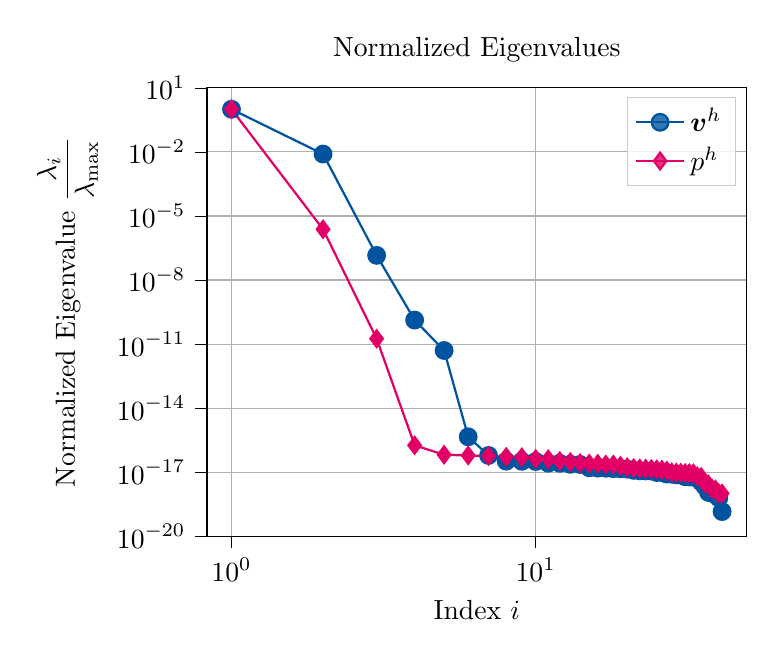
\begin{tikzpicture}

\definecolor{color0}{rgb}{0,0.329411764705882,0.623529411764706}
\definecolor{color1}{rgb}{0.890196078431372,0,0.4}

\begin{axis}[
legend cell align={left},
legend style={fill opacity=0.8, draw opacity=1, text opacity=1, draw=white!80!black},
log basis x={10},
log basis y={10},
tick align=outside,
tick pos=left,
title={Normalized Eigenvalues},
x grid style={white!69.0196078431373!black},
xlabel={Index \(\displaystyle i\)},
xmajorgrids,
xmin=0.830540485032707, xmax=49.3654442364545,
xmode=log,
xtick style={color=black},
xtick={0.01,0.1,1,10,100,1000},
xticklabels={
  \(\displaystyle 10^{-2}\),
  \(\displaystyle 10^{-1}\),
  \(\displaystyle 10^{0}\),
  \(\displaystyle 10^{1}\),
  \(\displaystyle 10^{2}\),
  \(\displaystyle 10^{3}\)
},
y grid style={white!69.0196078431373!black},
ylabel={Normalized Eigenvalue \(\displaystyle \frac{\lambda_i}{\lambda_{\text{max}}}\)},
ymajorgrids,
ymin=1e-20, ymax=10,
ymode=log,
ytick style={color=black},
ytick={1e-23,1e-20,1e-17,1e-14,1e-11,1e-08,1e-05,0.01,10,10000},
yticklabels={
  \(\displaystyle 10^{-23}\),
  \(\displaystyle 10^{-20}\),
  \(\displaystyle 10^{-17}\),
  \(\displaystyle 10^{-14}\),
  \(\displaystyle 10^{-11}\),
  \(\displaystyle 10^{-8}\),
  \(\displaystyle 10^{-5}\),
  \(\displaystyle 10^{-2}\),
  \(\displaystyle 10^{1}\),
  \(\displaystyle 10^{4}\)
}
]
\addplot [thick, color0, mark=*, mark size=3, mark options={solid}]
table {%
1 1
2 0.00794975858415845
3 1.42582257382325e-07
4 1.32791974403868e-10
5 5.00366283890635e-12
6 4.54114155240754e-16
7 6.04573529497411e-17
8 3.26201133022688e-17
9 3.22574638852698e-17
10 3.15358446366046e-17
11 2.62454621731955e-17
12 2.60840954654917e-17
13 2.33242093571454e-17
14 2.28813585566599e-17
15 1.60218882337199e-17
16 1.54306862706516e-17
17 1.52807821353466e-17
18 1.44864745846082e-17
19 1.43851705211444e-17
20 1.38677194525787e-17
21 1.21734236816605e-17
22 1.14897279038485e-17
23 1.13956935268721e-17
24 1.12564920102658e-17
25 9.63808041350083e-18
26 9.58979066065725e-18
27 8.13046505587439e-18
28 8.00740202533402e-18
29 7.46188080562777e-18
30 7.26718042554605e-18
31 6.11314351785897e-18
32 5.93273799548898e-18
33 5.84970067761768e-18
34 5.29939613242502e-18
35 3.47549460184894e-18
36 2.1905261247255e-18
37 1.12228744856004e-18
38 1.01406198292573e-18
39 9.59373162820783e-19
40 6.26226288149959e-19
41 1.42523827201686e-19
};
\addlegendentry{$\trialVelocityHomDiscrete$}
\addplot [thick, color1, mark=diamond*, mark size=3, mark options={solid}]
table {%
1 1
2 2.37328846603967e-06
3 1.78817929292869e-11
4 1.81154657334976e-16
5 6.51678466039161e-17
6 6.02235881107004e-17
7 5.69247083103718e-17
8 5.20065737906182e-17
9 5.01348143603465e-17
10 4.20958043774671e-17
11 4.07622974109276e-17
12 3.32697934377648e-17
13 2.98511733192585e-17
14 2.64421964531683e-17
15 2.52583071694472e-17
16 2.48386648445979e-17
17 2.27569426656641e-17
18 2.27247846357554e-17
19 1.99821382141988e-17
20 1.70491132142761e-17
21 1.54624364513944e-17
22 1.49112670601225e-17
23 1.45406520529215e-17
24 1.40935012359226e-17
25 1.35426769923973e-17
26 1.2976308799412e-17
27 1.18179500955933e-17
28 9.80114361457536e-18
29 9.51423374282225e-18
30 9.36239599182889e-18
31 9.08584610553105e-18
32 8.96571848518543e-18
33 8.78366822577326e-18
34 6.40001828288954e-18
35 5.93546015704658e-18
36 2.97856912325833e-18
37 2.64216217074413e-18
38 1.67829393129063e-18
39 1.53977850304594e-18
40 1.02797999983454e-18
41 1.00473640799576e-18
};
\addlegendentry{$p^h$}
\end{axis}

\end{tikzpicture}

        }
    }
    \subcaptionbox{Maximum interpolation error during the \gls{eim}.\label{fig:valve-likeEIMErrors}}{
        \resizebox{0.44\textwidth}{!}{
        % This file was created by tikzplotlib v0.9.8.
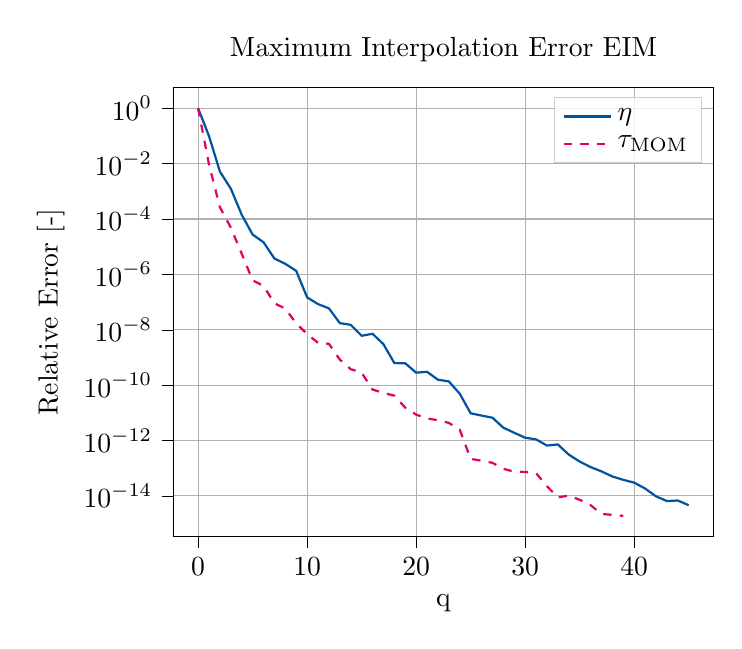
\begin{tikzpicture}

%\definecolor{color0}{rgb}{0.12156862745098,0.466666666666667,0.705882352941177}
%\definecolor{color1}{rgb}{1,0.498039215686275,0.0549019607843137}

\definecolor{color0}{rgb}{0,0.329411764705882,0.623529411764706}
\definecolor{color1}{rgb}{0.890196078431372,0,0.4}

\begin{axis}[
legend cell align={left},
legend style={fill opacity=0.8, draw opacity=1, text opacity=1, draw=white!80!black},
log basis y={10},
tick align=outside,
tick pos=left,
title={Maximum Interpolation Error EIM},
x grid style={white!69.0196078431373!black},
xlabel={q},
xmajorgrids,
xmin=-2.25, xmax=47.25,
xtick style={color=black},
xtick={-10,0,10,20,30,40,50},
xticklabels={
  \(\displaystyle -10\),
  \(\displaystyle 0\),
  \(\displaystyle 10\),
  \(\displaystyle 20\),
  \(\displaystyle 30\),
  \(\displaystyle 40\),
  \(\displaystyle 50\)
},
y grid style={white!69.0196078431373!black},
ylabel={Relative Error [-]},
ymajorgrids,
ymin=3.51471410776371e-16, ymax=5.44389825525944,
ymode=log,
ytick style={color=black},
ytick={1e-18,1e-16,1e-14,1e-12,1e-10,1e-08,1e-06,0.0001,0.01,1,100,10000},
yticklabels={
  \(\displaystyle 10^{-18}\),
  \(\displaystyle 10^{-16}\),
  \(\displaystyle 10^{-14}\),
  \(\displaystyle 10^{-12}\),
  \(\displaystyle 10^{-10}\),
  \(\displaystyle 10^{-8}\),
  \(\displaystyle 10^{-6}\),
  \(\displaystyle 10^{-4}\),
  \(\displaystyle 10^{-2}\),
  \(\displaystyle 10^{0}\),
  \(\displaystyle 10^{2}\),
  \(\displaystyle 10^{4}\)
}
]
\addplot [thick, color0]
table {%
0 1
1 0.0987673453717658
2 0.00515599137631726
3 0.00124900271315819
4 0.000142463479281955
5 2.74366574975223e-05
6 1.44975700969233e-05
7 3.73748485858245e-06
8 2.40757494835904e-06
9 1.34040458242958e-06
10 1.47604939852668e-07
11 8.49109837914781e-08
12 5.91845957000327e-08
13 1.74224683009756e-08
14 1.51054092822489e-08
15 6.07435279360086e-09
16 7.16579464736882e-09
17 3.01910092646183e-09
18 6.27830508569281e-10
19 6.15982655829241e-10
20 2.83140648375761e-10
21 3.03192480175683e-10
22 1.57506587196689e-10
23 1.36631157416829e-10
24 4.91399776836732e-11
25 9.63959118288821e-12
26 7.98281605427662e-12
27 6.6676277667823e-12
28 2.91438313811172e-12
29 1.90614931246576e-12
30 1.26634505351022e-12
31 1.10023595172808e-12
32 6.60646845871169e-13
33 7.2149035717033e-13
34 3.11375616648648e-13
35 1.74109286658845e-13
36 1.10318338826161e-13
37 7.70544122335398e-14
38 5.03169522508634e-14
39 3.8106143754838e-14
40 3.02112244686146e-14
41 1.85267439250041e-14
42 9.68443432443396e-15
43 6.52646660994462e-15
44 6.84226338139356e-15
45 4.63168598125102e-15
};
\addlegendentry{$\eta$}
\addplot [thick, dashed, color1]
table {%
0 1
1 0.00932238039336628
2 0.000266943760459508
3 4.90949857038112e-05
4 5.599960695831e-06
5 6.12824410476193e-07
6 3.86211523959076e-07
7 9.04010167944746e-08
8 5.82744632540993e-08
9 1.70168470184833e-08
10 7.04436726456646e-09
11 3.36213438130085e-09
12 3.11207201674506e-09
13 8.38932040992142e-10
14 3.78263928821779e-10
15 2.82163428907021e-10
16 6.95533441664873e-11
17 5.24268227949716e-11
18 4.19121093616782e-11
19 1.54370265480439e-11
20 8.64749152149743e-12
21 6.24447738563931e-12
22 5.44681941832098e-12
23 4.3396799607452e-12
24 2.47660431675892e-12
25 2.18757513175438e-13
26 1.86329799904232e-13
27 1.57026268596924e-13
28 9.55790405605825e-14
29 7.48084623843346e-14
30 7.36848530815293e-14
31 6.64897673464922e-14
32 2.24123930998593e-14
33 8.85932301724094e-15
34 1.03441814307043e-14
35 7.2349477058683e-15
36 4.64890234819224e-15
37 2.2322703665489e-15
38 2.07282248322398e-15
39 1.91337459989906e-15
};
\addlegendentry{$\tMomPlain$}
\end{axis}

\end{tikzpicture}

        }
    }
    \caption{Valve-like test case: results from the construction of the \gls{rom}.}
    \label{fig:valve-likeOffline}
\end{figure}
\bigskip
\par
To quantify the quality of the \gls{rom}, we perform an error and performance analysis. To that end, we create $\nTest = 50$ testing samples drawn from a uniform distribution. For each sample, we compare the solutions from the \gls{fom} and the \gls{rom} as well as the respective runtimes.
To evaluate the accuracy of the \gls{rom}, we use the following error definitions:
\begin{align}
    \relErrorVelocity
    =
    \frac
    {|\trialVelocityDiscrete-\trialVelocityReduced|_{\sobolevSpaceVector}}
    {|\trialVelocityDiscrete|_{\sobolevSpaceVector}},
    \,
    \relErrorPressure
    =
    \frac
    {||\trialPressureDiscrete-\trialPressureReduced||_{L^2}}
    {||\trialPressureDiscrete||_{L^2}},
\end{align}
where $|\cdot|_{\sobolevSpaceVector}$ and $||\cdot||_{L^2}$ are discrete measures for the $\sobolevSpaceVector$ semi-norm and the $L^2$ norm, respectively. The maximal error over all testing samples is shown in \Cref{fig:valveRelativeErrorMax}, using different numbers of basis functions for the velocity and the pressure field. Note that we ignore the lifting function in these plots, since it does not represent a solution, but is only intended to ensure the Dirichlet boundary conditions.
For the velocity, the error ranges from values smaller than \SI{1e-2}{} to values smaller than \SI{1e-6}{} when increasing the number of basis functions. Similarly, the maximum error in the pressure is limited by \SI{1e-2}{} and drops below \SI{1e-7}{} for $\nBasisVelocityROM$ and $\nBasisPressureROM$ large enough. These results suggest that the error introduced by the \gls{rom} is in a reasonable range for typical engineering applications and, furthermore, that it can be controlled by choosing the number of basis functions such that a desired accuracy is achieved.
\begin{figure}
    \captionsetup[sub]{position=bottom}
    \centering
    \Large
    \subcaptionbox{Velocity.}{
        \resizebox{0.44\textwidth}{!}{
        % This file was created by tikzplotlib v0.9.8.
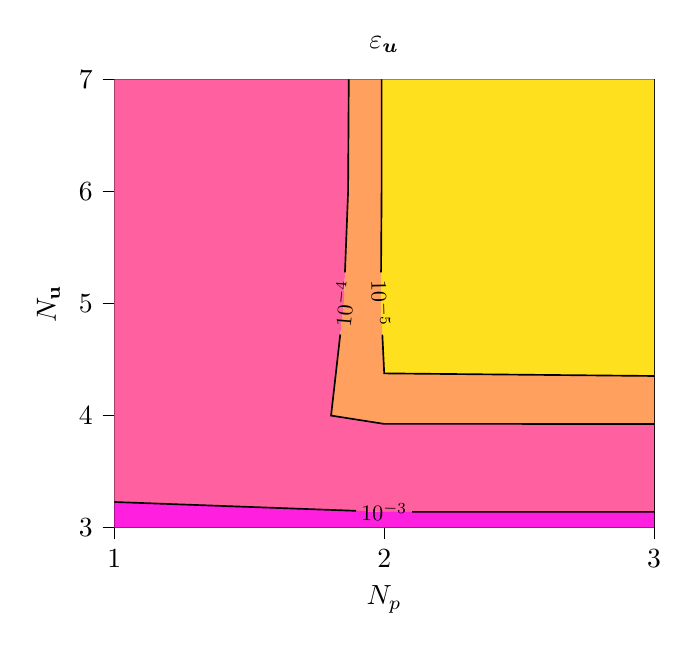
\begin{tikzpicture}

\definecolor{color0}{rgb}{1,0.87843137254902,0.12156862745098}
\definecolor{color1}{rgb}{1,0.627450980392157,0.372549019607843}
\definecolor{color2}{rgb}{1,0.376470588235294,0.623529411764706}
\definecolor{color3}{rgb}{1,0.125490196078431,0.874509803921569}

\begin{axis}[
tick align=outside,
tick pos=left,
%title={Relative Error in Velocity \(\displaystyle \mathbf{u}\) - Max},
title={$\relErrorVelocity$},
x grid style={white!69.0196078431373!black},
xlabel={\(\displaystyle N_p\)},
xmin=1, xmax=3,
xtick style={color=black},
xtick={1,2,3},
xticklabels={\(\displaystyle 1\),\(\displaystyle 2\),\(\displaystyle 3\)},
y grid style={white!69.0196078431373!black},
ylabel={\(\displaystyle N_{\mathbf{u}}\)},
ymin=3, ymax=7,
ytick style={color=black},
ytick={3,4,5,6,7},
yticklabels={
  \(\displaystyle 3\),
  \(\displaystyle 4\),
  \(\displaystyle 5\),
  \(\displaystyle 6\),
  \(\displaystyle 7\)
}
]
\addplot [draw=none, fill=color0]
table{%
x  y
2 4.37650891394412
3 4.35330770412385
3 5
3 6
3 7
2 7
1.99040991259345 7
1.9903127173998 6
1.98760845108052 5
2 4.37650891394412
};
\addplot [draw=none, fill=color1]
table{%
x  y
2 3.92579367910137
3 3.92540471448223
3 4
3 4.35330770412385
2 4.37650891394412
1.98760845108052 5
1.9903127173998 6
1.99040991259345 7
1.86869012295147 7
1.86619036626405 6
1.85013870710813 5
1.80309130655496 4
2 3.92579367910137
};
\addplot [draw=none, fill=color2]
table{%
x  y
2 3.14101234840689
3 3.14081265825156
3 3.92540471448223
2 3.92579367910137
1.80309130655496 4
1.85013870710813 5
1.86619036626405 6
1.86869012295147 7
1 7
1 6
1 5
1 4
1 3.22895886838152
2 3.14101234840689
};
\addplot [draw=none, fill=color3]
table{%
x  y
2 3
3 3
3 3.14081265825156
2 3.14101234840689
1 3.22895886838152
1 3
2 3
};
\path [draw=black, semithick]
(axis cs:3,4.35330770412385)
--(axis cs:2,4.37650891394412)
--(axis cs:1.99313704618645,4.72182414084339);

\path [draw=black, semithick]
(axis cs:1.98836176234379,5.27856400751013)
--(axis cs:1.9903127173998,6)
--(axis cs:1.99040991259345,7);

\path [draw=black, semithick]
(axis cs:3,3.92540471448223)
--(axis cs:2,3.92579367910137)
--(axis cs:1.80309130655496,4)
--(axis cs:1.83713590577805,4.72362338456115);

\path [draw=black, semithick]
(axis cs:1.85460609537104,5.27831317744237)
--(axis cs:1.86619036626405,6)
--(axis cs:1.86869012295147,7);

\path [draw=black, semithick]
(axis cs:3,3.14081265825156)
--(axis cs:2.10379029115697,3.14099162250753);

\path [draw=black, semithick]
(axis cs:1.89626538289669,3.15013544698203)
--(axis cs:1,3.22895886838152);

\draw (axis cs:1.98760845108052,5) node[
  scale=0.8,
  text=black,
  rotate=271.3
]{$10^{-5}$};
\draw (axis cs:1.85013870710813,5) node[
  scale=0.8,
  text=black,
  rotate=85.2
]{$10^{-4}$};
\draw (axis cs:2,3.14101234840689) node[
  scale=0.8,
  text=black,
  rotate=359.1
]{$10^{-3}$};
\end{axis}

\end{tikzpicture}
}
    }
    \subcaptionbox{Pressure.}{
        \resizebox{0.44\textwidth}{!}{
        % This file was created by tikzplotlib v0.9.8.
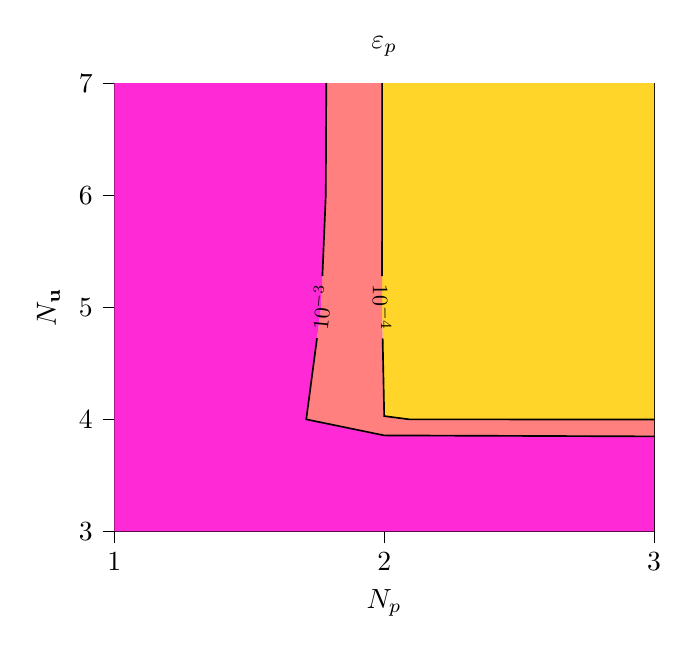
\begin{tikzpicture}

\definecolor{color0}{rgb}{1,0.835294117647059,0.164705882352941}
\definecolor{color1}{rgb}{1,0.501960784313725,0.498039215686275}
\definecolor{color2}{rgb}{1,0.164705882352941,0.835294117647059}

\begin{axis}[
tick align=outside,
tick pos=left,
%title={Relative Error in Pressure \(\displaystyle p\) - Max},
title={$\relErrorPressure$},
x grid style={white!69.0196078431373!black},
xlabel={\(\displaystyle N_p\)},
xmin=1, xmax=3,
xtick style={color=black},
xtick={1,2,3},
xticklabels={\(\displaystyle 1\),\(\displaystyle 2\),\(\displaystyle 3\)},
y grid style={white!69.0196078431373!black},
ylabel={\(\displaystyle N_{\mathbf{u}}\)},
ymin=3, ymax=7,
ytick style={color=black},
ytick={3,4,5,6,7},
yticklabels={
  \(\displaystyle 3\),
  \(\displaystyle 4\),
  \(\displaystyle 5\),
  \(\displaystyle 6\),
  \(\displaystyle 7\)
}
]
\addplot [draw=none, fill=color0]
table{%
x  y
3 3.99841272096808
3 4
3 5
3 6
3 7
2 7
1.99231388686608 7
1.9923086500537 6
1.99186016592534 5
2 4.02906689026844
2.0929081054864 4
3 3.99841272096808
};
\addplot [draw=none, fill=color1]
table{%
x  y
2 3.85666988114318
3 3.84783564712328
3 3.99841272096808
2.0929081054864 4
2 4.02906689026844
1.99186016592534 5
1.9923086500537 6
1.99231388686608 7
1.78528526361933 7
1.78346767600251 6
1.76616198020346 5
1.71107969290604 4
2 3.85666988114318
};
\addplot [draw=none, fill=color2]
table{%
x  y
2 3
3 3
3 3.84783564712328
2 3.85666988114318
1.71107969290604 4
1.76616198020346 5
1.78346767600251 6
1.78528526361933 7
1 7
1 6
1 5
1 4
1 3
2 3
};
\path [draw=black, semithick]
(axis cs:3,3.99841272096808)
--(axis cs:2.0929081054864,4)
--(axis cs:2,4.02906689026844)
--(axis cs:1.99419498249751,4.72149914921187);

\path [draw=black, semithick]
(axis cs:1.99198510066168,5.278571143184)
--(axis cs:1.9923086500537,6)
--(axis cs:1.99231388686608,7);

\path [draw=black, semithick]
(axis cs:3,3.84783564712328)
--(axis cs:2,3.85666988114318)
--(axis cs:1.71107969290604,4)
--(axis cs:1.75098262156661,4.72442395946829);

\path [draw=black, semithick]
(axis cs:1.77097765920204,5.27827133069329)
--(axis cs:1.78346767600251,6)
--(axis cs:1.78528526361933,7);

\draw (axis cs:1.99186016592534,5) node[
  scale=0.8,
  text=black,
  rotate=270.6
]{$10^{-4}$};
\draw (axis cs:1.76616198020346,5) node[
  scale=0.8,
  text=black,
  rotate=84.5
]{$10^{-3}$};
\end{axis}

\end{tikzpicture}
}
    }
    \caption{Valve-like test case: maximum relative error of the \gls{rom} over all testing samples.}
    \label{fig:valveRelativeErrorMax}
\end{figure}
\par
Finally, we investigate the performance of the \gls{rom} by comparing the CPU time needed for a single evaluation of the \gls{rom} to that for the \gls{fom}. Note that the former has been run on a single core, whereas the latter used 64 cores. Also in this analysis, we skip the lifting function for the same reason as before. \Cref{fig:valvePerformance} presents the speed up, i.e., the ratio between the CPU time of \gls{fom} and \gls{rom} evaluations, for different number of basis functions $\nBasisVelocityROM$ and $\nBasisPressureROM$.  Both, the average and the maximum speed up, are in the order of 1000 and indicate that a significant reduction of the runtime for the \gls{rom} is realized. 
\begin{figure}
    \captionsetup[sub]{position=bottom}
    \centering
    \Large
    \subcaptionbox{Average speed up over all testing samples.}{
        \resizebox{0.44\textwidth}{!}{
        % This file was created by tikzplotlib v0.9.8.
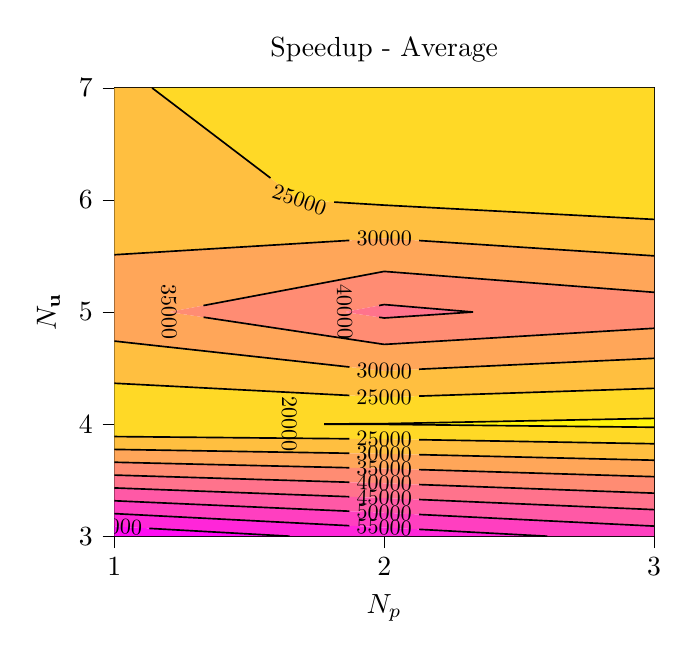
\begin{tikzpicture}

\definecolor{color0}{rgb}{1,0.952941176470588,0.0470588235294118}
\definecolor{color1}{rgb}{1,0.850980392156863,0.149019607843137}
\definecolor{color2}{rgb}{1,0.749019607843137,0.250980392156863}
\definecolor{color3}{rgb}{1,0.650980392156863,0.349019607843137}
\definecolor{color4}{rgb}{1,0.549019607843137,0.450980392156863}
\definecolor{color5}{rgb}{1,0.450980392156863,0.549019607843137}
\definecolor{color6}{rgb}{1,0.349019607843137,0.650980392156863}
\definecolor{color7}{rgb}{1,0.247058823529412,0.752941176470588}
\definecolor{color8}{rgb}{1,0.149019607843137,0.850980392156863}
\definecolor{color9}{rgb}{1,0.0470588235294118,0.952941176470588}

\begin{axis}[
tick align=outside,
tick pos=left,
title={Speedup - Average},
x grid style={white!69.0196078431373!black},
xlabel={\(\displaystyle N_p\)},
xmin=1, xmax=3,
xtick style={color=black},
xtick={1,2,3},
xticklabels={\(\displaystyle 1\),\(\displaystyle 2\),\(\displaystyle 3\)},
y grid style={white!69.0196078431373!black},
ylabel={\(\displaystyle N_{\mathbf{u}}\)},
ymin=3, ymax=7,
ytick style={color=black},
ytick={3,4,5,6,7},
yticklabels={
  \(\displaystyle 3\),
  \(\displaystyle 4\),
  \(\displaystyle 5\),
  \(\displaystyle 6\),
  \(\displaystyle 7\)
}
]
\addplot [draw=none, fill=color0]
table{%
x  y
2 3.99776029877739
3 3.97186061500088
3 4
3 4.05129247948725
2 4.00401665310977
1.64783776122399 4
2 3.99776029877739
};
\addplot [draw=none, fill=color1]
table{%
x  y
2 3.86632751738316
3 3.82489079580478
3 3.97186061500088
2 3.99776029877739
1.64783776122399 4
2 4.00401665310977
3 4.05129247948725
3 4.31918911036938
2 4.23972661512697
1 4.36447852644752
1 4
1 3.88899847255399
2 3.86632751738316
};
\addplot [draw=none, fill=color1]
table{%
x  y
2 5.95377752187074
3 5.82647002301902
3 6
3 7
2 7
1.13955470147603 7
1.68538959041588 6
2 5.95377752187074
};
\addplot [draw=none, fill=color2]
table{%
x  y
2 3.73489473598894
3 3.67792097660869
3 3.82489079580478
2 3.86632751738316
1 3.88899847255399
1 3.77440465802077
2 3.73489473598894
};
\addplot [draw=none, fill=color2]
table{%
x  y
2 4.23972661512697
3 4.31918911036938
3 4.58708574125151
2 4.47543657714418
1 4.74075248971692
1 4.36447852644752
2 4.23972661512697
};
\addplot [draw=none, fill=color2]
table{%
x  y
2 5.65807486026756
3 5.50125704822069
3 5.82647002301902
2 5.95377752187074
1.68538959041588 6
1.13955470147603 7
1 7
1 6
1 5.51094647432634
2 5.65807486026756
};
\addplot [draw=none, fill=color3]
table{%
x  y
2 3.60346195459471
3 3.5309511574126
3 3.67792097660869
2 3.73489473598894
1 3.77440465802077
1 3.65981084348756
2 3.60346195459471
};
\addplot [draw=none, fill=color3]
table{%
x  y
2 4.47543657714418
3 4.58708574125151
3 4.85498237213365
2 4.71114653916139
1.20242039825908 5
2 5.36237219866437
3 5.17604407342235
3 5.50125704822069
2 5.65807486026756
1 5.51094647432634
1 5
1 4.74075248971692
2 4.47543657714418
};
\addplot [draw=none, fill=color4]
table{%
x  y
2 3.47202917320049
3 3.38398133821651
3 3.5309511574126
2 3.60346195459471
1 3.65981084348756
1 3.54521702895434
2 3.47202917320049
};
\addplot [draw=none, fill=color4]
table{%
x  y
2 4.71114653916139
3 4.85498237213365
3 5
3 5.17604407342235
2 5.36237219866437
1.20242039825908 5
2 4.71114653916139
1.85326064468108 5
2 5.06666953706118
2.3295534889383 5
2 4.94685650117859
1.85326064468108 5
};
\addplot [draw=none, fill=color5]
table{%
x  y
2 3.34059639180626
3 3.23701151902041
3 3.38398133821651
2 3.47202917320049
1 3.54521702895434
1 3.43062321442112
2 3.34059639180626
};
\addplot [draw=none, fill=color5]
table{%
x  y
2 4.94685650117859
2.3295534889383 5
2 5.06666953706118
1.85326064468108 5
2 4.94685650117859
};
\addplot [draw=none, fill=color6]
table{%
x  y
2 3.20916361041203
3 3.09004169982432
3 3.23701151902041
2 3.34059639180626
1 3.43062321442112
1 3.3160293998879
2 3.20916361041203
};
\addplot [draw=none, fill=color7]
table{%
x  y
2 3.07773082901781
2.60424735056556 3
3 3
3 3.09004169982432
2 3.20916361041203
1 3.3160293998879
1 3.20143558535469
2 3.07773082901781
};
\addplot [draw=none, fill=color8]
table{%
x  y
2 3
2.60424735056556 3
2 3.07773082901781
1 3.20143558535469
1 3.08684177082147
1.64970439596316 3
2 3
};
\addplot [draw=none, fill=color9]
table{%
x  y
1 3.08684177082147
1 3
1.64970439596316 3
1 3.08684177082147
};
\path [draw=black, semithick]
(axis cs:3,3.97186061500088)
--(axis cs:2,3.99776029877739)
--(axis cs:1.77726149904818,3.99917688362941);

\path [draw=black, semithick]
(axis cs:1.77726069380053,4.00147615776869)
--(axis cs:2,4.00401665310977)
--(axis cs:3,4.05129247948725);

\path [draw=black, semithick]
(axis cs:3,3.82489079580478)
--(axis cs:2.12940867994302,3.86096524594254);

\path [draw=black, semithick]
(axis cs:1.87058051564284,3.86926158071125)
--(axis cs:1,3.88899847255399);

\path [draw=black, semithick]
(axis cs:1,4.36447852644752)
--(axis cs:1.87071547689406,4.2558551064886);

\path [draw=black, semithick]
(axis cs:2.12936741661236,4.25000647285406)
--(axis cs:3,4.31918911036938);

\path [draw=black, semithick]
(axis cs:3,5.82647002301902)
--(axis cs:2,5.95377752187074)
--(axis cs:1.81462022259509,5.98101346971504);

\path [draw=black, semithick]
(axis cs:1.57849420274952,6.1958383200348)
--(axis cs:1.13955470147603,7);

\path [draw=black, semithick]
(axis cs:3,3.67792097660869)
--(axis cs:2.1293949518265,3.72752261913855);

\path [draw=black, semithick]
(axis cs:1.87058991946085,3.74000771818117)
--(axis cs:1,3.77440465802077);

\path [draw=black, semithick]
(axis cs:1,4.74075248971692)
--(axis cs:1.87120364443596,4.5096082997567);

\path [draw=black, semithick]
(axis cs:2.12931226725914,4.48987418369249)
--(axis cs:3,4.58708574125151);

\path [draw=black, semithick]
(axis cs:3,5.50125704822069)
--(axis cs:2.12920375458042,5.63781341016601);

\path [draw=black, semithick]
(axis cs:1.87076991649158,5.63906144666591)
--(axis cs:1,5.51094647432634);

\path [draw=black, semithick]
(axis cs:3,3.5309511574126)
--(axis cs:2.12937689557672,3.5940807327595);

\path [draw=black, semithick]
(axis cs:1.87060441248816,3.61075325217864)
--(axis cs:1,3.65981084348756);

\path [draw=black, semithick]
(axis cs:3,5.17604407342235)
--(axis cs:2,5.36237219866437)
--(axis cs:1.33002909148532,5.05797771486651);

\path [draw=black, semithick]
(axis cs:1.33068211116719,4.95354841123603)
--(axis cs:2,4.71114653916139)
--(axis cs:3,4.85498237213365);

\path [draw=black, semithick]
(axis cs:3,3.38398133821651)
--(axis cs:2.12935451663035,3.46063978806578);

\path [draw=black, semithick]
(axis cs:1.87062398959549,3.48149792598798)
--(axis cs:1,3.54521702895434);

\path [draw=black, semithick]
(axis cs:1.98152235758919,4.95354841123603)
--(axis cs:2,4.94685650117859)
--(axis cs:2.3295534889383,5)
--(axis cs:2,5.06666953706118)
--(axis cs:1.98086933790731,5.05797771486651);

\path [draw=black, semithick]
(axis cs:3,3.23701151902041)
--(axis cs:2.12932782172,3.32719998584572);

\path [draw=black, semithick]
(axis cs:1.87064864385909,3.35224148340055)
--(axis cs:1,3.43062321442112);

\path [draw=black, semithick]
(axis cs:3,3.09004169982432)
--(axis cs:2.12929681886861,3.19376152631549);

\path [draw=black, semithick]
(axis cs:1.87067836656755,3.2229836688651)
--(axis cs:1,3.3160293998879);

\path [draw=black, semithick]
(axis cs:2.60424735056556,3)
--(axis cs:2.12927570066499,3.06110070664302);

\path [draw=black, semithick]
(axis cs:1.87071314723031,3.09372422763725)
--(axis cs:1,3.20143558535469);

\path [draw=black, semithick]
(axis cs:1.64970439596316,3)
--(axis cs:1.12926390778472,3.06956390303255);

\draw (axis cs:1.64783776122399,4) node[
  scale=0.8,
  text=black,
  rotate=270.1
]{20000};
\draw (axis cs:2,3.86632751738316) node[
  scale=0.8,
  text=black,
  rotate=359.3
]{25000};
\draw (axis cs:2,4.23972661512697) node[
  scale=0.8,
  text=black,
  rotate=359.5
]{25000};
\draw (axis cs:1.68538959041588,6) node[
  scale=0.8,
  text=black,
  rotate=341.3
]{25000};
\draw (axis cs:2,3.73489473598894) node[
  scale=0.8,
  text=black,
  rotate=359.0
]{30000};
\draw (axis cs:2,4.47543657714418) node[
  scale=0.8,
  text=black,
  rotate=358.4
]{30000};
\draw (axis cs:2,5.65807486026756) node[
  scale=0.8,
  text=black,
  rotate=359.9
]{30000};
\draw (axis cs:2,3.60346195459471) node[
  scale=0.8,
  text=black,
  rotate=358.6
]{35000};
\draw (axis cs:1.20242039825908,5) node[
  scale=0.8,
  text=black,
  rotate=271.0
]{35000};
\draw (axis cs:2,3.47202917320049) node[
  scale=0.8,
  text=black,
  rotate=358.3
]{40000};
\draw (axis cs:1.85326064468108,5) node[
  scale=0.8,
  text=black,
  rotate=271.0
]{40000};
\draw (axis cs:2,3.34059639180626) node[
  scale=0.8,
  text=black,
  rotate=357.9
]{45000};
\draw (axis cs:2,3.20916361041203) node[
  scale=0.8,
  text=black,
  rotate=357.6
]{50000};
\draw (axis cs:2,3.07773082901781) node[
  scale=0.8,
  text=black,
  rotate=357.3
]{55000};
\draw (axis cs:1,3.08684177082147) node[
  scale=0.8,
  text=black,
  rotate=357.1
]{60000};
\end{axis}

\end{tikzpicture}
}
    }
    \subcaptionbox{Maximum speed up over all testing samples.}{
        \resizebox{0.44\textwidth}{!}{
        % This file was created by tikzplotlib v0.9.8.
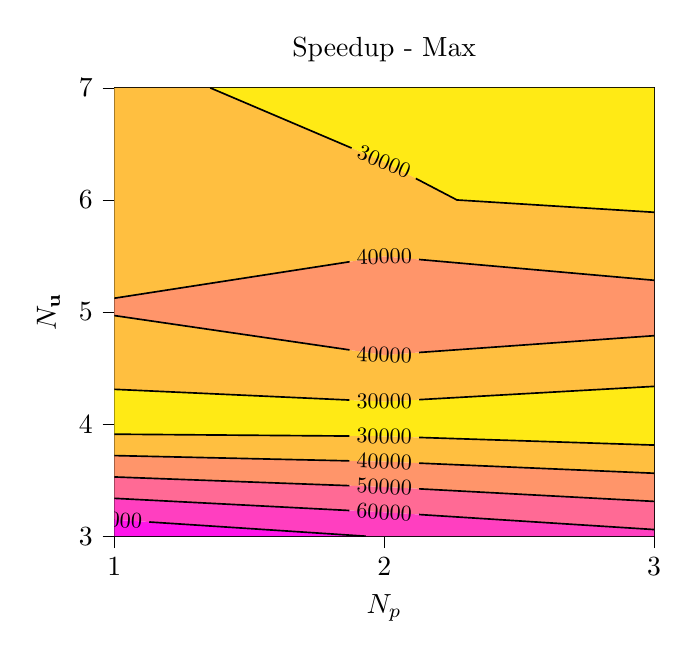
\begin{tikzpicture}

\definecolor{color0}{rgb}{1,0.917647058823529,0.0823529411764706}
\definecolor{color1}{rgb}{1,0.749019607843137,0.250980392156863}
\definecolor{color2}{rgb}{1,0.584313725490196,0.415686274509804}
\definecolor{color3}{rgb}{1,0.415686274509804,0.584313725490196}
\definecolor{color4}{rgb}{1,0.247058823529412,0.752941176470588}
\definecolor{color5}{rgb}{1,0.0823529411764706,0.917647058823529}

\begin{axis}[
tick align=outside,
tick pos=left,
title={Speedup - Max},
x grid style={white!69.0196078431373!black},
xlabel={\(\displaystyle N_p\)},
xmin=1, xmax=3,
xtick style={color=black},
xtick={1,2,3},
xticklabels={\(\displaystyle 1\),\(\displaystyle 2\),\(\displaystyle 3\)},
y grid style={white!69.0196078431373!black},
ylabel={\(\displaystyle N_{\mathbf{u}}\)},
ymin=3, ymax=7,
ytick style={color=black},
ytick={3,4,5,6,7},
yticklabels={
  \(\displaystyle 3\),
  \(\displaystyle 4\),
  \(\displaystyle 5\),
  \(\displaystyle 6\),
  \(\displaystyle 7\)
}
]
\addplot [draw=none, fill=color0]
table{%
x  y
2 3.89113969366561
3 3.81295761379902
3 4
3 4.33664393194555
2 4.20059943824401
1 4.31046717020061
1 4
1 3.91000519290614
2 3.89113969366561
};
\addplot [draw=none, fill=color0]
table{%
x  y
3 5.8901285826523
3 6
3 7
2 7
1.35534430289395 7
2 6.33923453361608
2.26948248989546 6
3 5.8901285826523
};
\addplot [draw=none, fill=color1]
table{%
x  y
2 3.66515692779255
3 3.56174755756104
3 3.81295761379902
2 3.89113969366561
1 3.91000519290614
1 3.71929144543007
2 3.66515692779255
};
\addplot [draw=none, fill=color1]
table{%
x  y
2 4.20059943824401
3 4.33664393194555
3 4.78877856727545
2 4.61702317811216
1 4.96839799320352
1 4.31046717020061
2 4.20059943824401
};
\addplot [draw=none, fill=color1]
table{%
x  y
2 5.49635319629926
3 5.28342883044444
3 5.8901285826523
2.26948248989546 6
2 6.33923453361608
1.35534430289395 7
1 7
1 6
1 5.12326574274158
2 5.49635319629926
};
\addplot [draw=none, fill=color2]
table{%
x  y
2 3.4391741619195
3 3.31053750132306
3 3.56174755756104
2 3.66515692779255
1 3.71929144543007
1 3.52857769795399
2 3.4391741619195
};
\addplot [draw=none, fill=color2]
table{%
x  y
2 4.61702317811216
3 4.78877856727545
3 5
3 5.28342883044444
2 5.49635319629926
1 5.12326574274158
1 5
1 4.96839799320352
2 4.61702317811216
};
\addplot [draw=none, fill=color3]
table{%
x  y
2 3.21319139604645
3 3.05932744508508
3 3.31053750132306
2 3.4391741619195
1 3.52857769795399
1 3.33786395047791
2 3.21319139604645
};
\addplot [draw=none, fill=color4]
table{%
x  y
2 3
3 3
3 3.05932744508508
2 3.21319139604645
1 3.33786395047791
1 3.14715020300184
1.93165335182826 3
2 3
};
\addplot [draw=none, fill=color5]
table{%
x  y
1 3.14715020300184
1 3
1.93165335182826 3
1 3.14715020300184
};
\path [draw=black, semithick]
(axis cs:3,3.81295761379902)
--(axis cs:2.12936922751048,3.8810253383881);

\path [draw=black, semithick]
(axis cs:1.87057909585802,3.89358128363441)
--(axis cs:1,3.91000519290614);

\path [draw=black, semithick]
(axis cs:1,4.31046717020061)
--(axis cs:1.87068419689434,4.21480707223737);

\path [draw=black, semithick]
(axis cs:2.12925816089073,4.21818429929918)
--(axis cs:3,4.33664393194555);

\path [draw=black, semithick]
(axis cs:3,5.8901285826523)
--(axis cs:2.26948248989546,6)
--(axis cs:2.11717612375158,6.19172889157148);

\path [draw=black, semithick]
(axis cs:1.87909257266006,6.46316340444465)
--(axis cs:1.35534430289395,7);

\path [draw=black, semithick]
(axis cs:3,3.56174755756104)
--(axis cs:2.12932814733133,3.65178318552381);

\path [draw=black, semithick]
(axis cs:1.87060221616005,3.67216181440409)
--(axis cs:1,3.71929144543007);

\path [draw=black, semithick]
(axis cs:1,4.96839799320352)
--(axis cs:1.87167093357662,4.66211478009752);

\path [draw=black, semithick]
(axis cs:2.12915991192253,4.63920708904871)
--(axis cs:3,4.78877856727545);

\path [draw=black, semithick]
(axis cs:3,5.28342883044444)
--(axis cs:2.12901874905936,5.46888196097241);

\path [draw=black, semithick]
(axis cs:1.87180845969371,5.44852654095875)
--(axis cs:1,5.12326574274158);

\path [draw=black, semithick]
(axis cs:3,3.31053750132306)
--(axis cs:2.12927571007098,3.42254456627974);

\path [draw=black, semithick]
(axis cs:1.87064764090286,3.45073872021719)
--(axis cs:1,3.52857769795399);

\path [draw=black, semithick]
(axis cs:3,3.05932744508508)
--(axis cs:2.12921195720541,3.19331033379938);

\path [draw=black, semithick]
(axis cs:1.87071529966112,3.22930964988661)
--(axis cs:1,3.33786395047791);

\path [draw=black, semithick]
(axis cs:1.93165335182826,3)
--(axis cs:1.12920058312662,3.12674358717447);

\draw (axis cs:2,3.89113969366561) node[
  scale=0.8,
  text=black,
  rotate=359.0
]{30000};
\draw (axis cs:2,4.20059943824401) node[
  scale=0.8,
  text=black,
  rotate=0.3
]{30000};
\draw (axis cs:2,6.33923453361608) node[
  scale=0.8,
  text=black,
  rotate=337.0
]{30000};
\draw (axis cs:2,3.66515692779255) node[
  scale=0.8,
  text=black,
  rotate=358.3
]{40000};
\draw (axis cs:2,4.61702317811216) node[
  scale=0.8,
  text=black,
  rotate=358.1
]{40000};
\draw (axis cs:2,5.49635319629926) node[
  scale=0.8,
  text=black,
  rotate=1.7
]{40000};
\draw (axis cs:2,3.4391741619195) node[
  scale=0.8,
  text=black,
  rotate=357.7
]{50000};
\draw (axis cs:2,3.21319139604645) node[
  scale=0.8,
  text=black,
  rotate=357.0
]{60000};
\draw (axis cs:1,3.14715020300184) node[
  scale=0.8,
  text=black,
  rotate=356.6
]{70000};
\end{axis}

\end{tikzpicture}
}
    }
    \caption{Valve-like test case: performance results.}
    \label{fig:valvePerformance}
\end{figure}
\par
Taken together, the error and performance analysis confirms the effectiveness of the approach for this two-dimensional deforming domain problem with topology changes. In particular, the accuracy of the \gls{rom} is acceptable as well as controllable while a significant reduction of the  computational demands is achieved, too. This qualifies the \gls{rom} as a surrogate model, e.g., in one of the aforementioned many query scenarios.   
\subsection{Artery-Like Geometry with Compression}
After presenting results for a spatially deforming two-dimensional geometry, we will now demonstrate the aptitude of the proposed approach also for the three-dimensional case, resulting in a four-dimensional space-time domain. The geometry is inspired by an artery that locally undergoes compression over time. The initial spatial geometry can be seen in \Cref{fig:arteryGeoInitialFront,fig:arteryGeoInitialSide,fig:arteryGeoInitialTop}. It has a length of $L = \SI{60e-3}{\meter}$ and a radius of $r_0 = \SI{5e-3}{\meter}$.
We are interested in the internal flow over a time period of $\SI{1}{\second}$ where fluid enters on the left-hand side, i.e., at $x_{\text{min}}$ .
The local narrowing of the artery happens according to the following expression for the upper and lower parts of the moving boundary:
\begin{align*}
    y(t) = \pm  \left[ 0.2 + 0.2 \cdot\left(\cos{(\pi\, t\,\si{\per\second})}+1\right)\right] \cdot r_0 .%, \, r_0 = \SI{5e-3}{\meter}. 
\end{align*}
The final state of the deformed spatial geometry is depicted in \Cref{fig:arteryGeoFinalSide,fig:arteryGeoFinalTop}.
\iffalse
Since we assume no-slip conditions along the walls, 
$x \in  [-\SI{30}{\milli\meter}, \SI{30}{\milli\meter}], \,  y \in [-\SI{5}{\milli\meter},\SI{5}{\milli\meter}], \, z \in [-\SI{5}{\milli\meter},\SI{5}{\milli\meter}], \, t \in [ \SI{0}{\second} ,\SI{1}{\second}]$. 
\fi
\par
To mimic blood, the density is set to $\density = \SI{1058}{\kilo\gram\per\cubic\meter}$ and the parameters for the viscosity model are chosen as presented in \cite{Cho1991}:
% etaZero 0.16 etaInf 0.0035 relaxTime 8.2 transRegionExponent 0.64 powerIndex 0.2128
\begin{align*}
    \visc_0 = \SI{0.056}{Pa\cdot s}, \,
    \visc_{\infty} = \SI{0.00345}{Pa\cdot s}, \,
    \lambda = \SI{1.902}{s}, \,
    a = \SI{1.25}{}, \,
    n = \SI{0.22}{}.
\end{align*}
\par
For the inflow velocity, we prescribe the following time-dependent profile:
%1.0e-1*(1-((sqrt(y*y+z*z)/0.005)*(sqrt(y*y+z*z)/0.005)))*(sqrt(t/0.2)*heaviside(0.2-t)+heaviside(t-0.2))
\begin{align*}
    \begin{aligned}
        \velX = \velX_{\text{in}}^0 \lp 1 - \frac{(y^2+z^2)}{r_0^2} \rp  \cdot 
        \begin{cases}  
            \sqrt{\frac{t}{\SI{0.2}{\second}}}    &\text{ for } t < \SI{0.2}{\second},
            \\
            1   &\text{ for } t \ge \SI{0.2}{\second},
        \end{cases}
    \end{aligned}
    \quad
    \begin{aligned}
        \velY = \SI{0}{\meter\per\second}, \quad \velZ = \SI{0}{\meter\per\second},       
    \end{aligned}
    \label{eq:artery-likeInflow}
\end{align*}
with the velocity vector $\trialVelocity = \lb \velX, \velY, \velZ \rb^T$ and $\velX_{\text{in}}^0=\SI{0.1}{\meter\per\second}$. At the outlet, a parallel outflow is enforced, i.e., $\velY=\velZ=0$. Along the walls, no-slip conditions are set. To account for the narrowing, we apply the following boundary conditions for the velocity in $y$-direction on the horizontal and rounded parts:
\begin{align}
   \velY = \frac{\partial y(t)}{\partial t} = \mp \pi \sin(\pi t)\times 10^{-3}\,\si{\meter\per\second}.% = \frac{\pi}{1000} \sin(\pi t) \, \si{\meter\per\second}
\end{align}
The sign of this term depends on whether you consider the upper or the lower part. In particular, the negative and the positive sign correspond to a downward movement for $y>0$ and an upward movement for $y<0$, respectively. 
For this geometry, a locally refined boundary-conforming simplex space-time mesh is constructed using a four-dimensional elastic mesh update~\cite{Danwitz2021}.
\Cref{fig:artery-likeVelocityInitial,fig:artery-likeVelocityFinal} show the resulting velocity field along the artery in its center plane for the initial and final state.
\newcommand{\myW}{0.48\textwidth} 
\begin{figure}
\captionsetup[sub]{position=bottom}
\centering
\subcaptionbox{Front view.\label{fig:arteryGeoInitialFront}}{
 %  \tikzsetnextfilename{topology-arteryFront}
   \begin{tikzpicture}[
    axis/.style={thick, ->},
    every node/.style={color=black}
    ]
       \node at (0,0) [inner sep=0pt, anchor=south west] {\includegraphics[width=\myW,trim={0cm 0cm 0cm 0cm},clip]{fig/artery-like/geometry/frontView/artery-like_3DGeometryFrontView.png}};
       \draw[axis] (0.2*\myW,0.05*\myW)  -- (0.3*\myW,0.05*\myW) node(xline)[right]{$z$};
       \draw[axis] (0.2*\myW,0.05*\myW)  -- (0.2*\myW,0.15*\myW) node(xline)[right]{$y$};
\end{tikzpicture}
}
\subcaptionbox{Side view at $t=0.0\,$s.\label{fig:arteryGeoInitialSide}}{
%\tikzsetnextfilename{topology-arterySide}
\begin{tikzpicture}[
    axis/.style={thick, ->},
    every node/.style={color=black}
    ]
       \node at (0,0) [inner sep=0pt, anchor=south west] {\includegraphics[width=\myW,trim={0cm 20cm 0cm 0cm},clip]{fig/artery-like/geometry/sideView/artery-like_3DSideView.0000.png}};
       \draw[axis] (0.1*\myW,0.05*\myW)  -- (0.2*\myW,0.05*\myW) node(xline)[right]{$x$};
       \draw[axis] (0.1*\myW,0.05*\myW)  -- (0.1*\myW,0.15*\myW) node(xline)[right]{$y$};
\end{tikzpicture}
}\subcaptionbox{Top view $t=0.0\,$s.\label{fig:arteryGeoInitialTop}}{
   %\tikzsetnextfilename{topology-arteryTop}
\begin{tikzpicture}[
    axis/.style={thick, ->},
    every node/.style={color=black}
    ]
       \node at (0,0) [inner sep=0pt, anchor=south west] {\includegraphics[width=\myW,trim={0cm 20cm 0cm 0cm},clip]{
       fig/artery-like/geometry/topView/artery-like_3DGeometryTopView.0000.png}};
       \draw[axis] (0.1*\myW,0.15*\myW)  -- (0.2*\myW,0.15*\myW) node(xline)[right]{$x$};
       \draw[axis] (0.1*\myW,0.15*\myW)  -- (0.1*\myW,0.05*\myW) node(xline)[right]{$z$};
\end{tikzpicture}
}\\
\subcaptionbox{Side view at $t=\SI{1}{\second}$.\label{fig:arteryGeoFinalSide}}{
 %   \tikzsetnextfilename{topology-arteryCSide}
\begin{tikzpicture}[
    axis/.style={thick, ->},
    every node/.style={color=black}
    ]
       \node at (0,0) [inner sep=0pt, anchor=south west] {\includegraphics[width=\myW,trim={0cm 20cm 0cm 0cm},clip]{fig/artery-like/geometry/sideView/artery-like_3DSideView.0034.png}};
       \draw[axis] (0.1*\myW,0.05*\myW)  -- (0.2*\myW,0.05*\myW) node(xline)[right]{$x$};
       \draw[axis] (0.1*\myW,0.05*\myW)  -- (0.1*\myW,0.15*\myW) node(xline)[right]{$y$};
\end{tikzpicture}
}\subcaptionbox{Top view at $t=\SI{1}{\second}$.\label{fig:arteryGeoFinalTop}}{
    % \tikzsetnextfilename{topology-arteryCTop}
 \begin{tikzpicture}[
    axis/.style={thick, ->},
    every node/.style={color=black}
    ]
       \node at (0,0) [inner sep=0pt, anchor=south west] {\includegraphics[width=\myW,trim={0cm 20cm 0cm 0cm},clip]{fig/artery-like/geometry/topView/artery-like_3DGeometryTopView.0034.png}};
       \draw[axis] (0.1*\myW,0.15*\myW)  -- (0.2*\myW,0.15*\myW) node(xline)[right]{$x$};
       \draw[axis] (0.1*\myW,0.15*\myW)  -- (0.1*\myW,0.05*\myW) node(xline)[right]{$z$};
\end{tikzpicture}
}
\caption{Artery-like test case: geometry.}
\label{fig:arteryGeo}
\end{figure}




%%%%%%%%%%%%%%%%%%%%%%%%%% BEGIN HIDDEN
\iffalse
\subsubsection{4D mesh generation}

The space-time finite element simulation of considered transient three-dimensional problem requires a four-dimensional mesh. To generate a four-dimensional pentatope mesh, we follow the procedure outlined in~\cite{danwitz2021four}. In this section, we describe the essential test case specific steps and provide reference with more details on the underlying algorithms.

\renewcommand{\myD}{0.9\textwidth}
\begin{figure}
\centering
% \tikzsetnextfilename{topology-arteryMesh}
\begin{tikzpicture}[
    axis/.style={very thick, ->},
    every node/.style={color=black}
    ]
       \node at (0,0) [inner sep=0pt, anchor=south west] {\includegraphics[width=\myD,trim={0cm 0cm 0cm 0cm},clip]{fig/artery-like/xyt}};
       \draw[axis] (0.014*\myD,0.434*\myD)  -- (0.11*\myD,0.45*\myD) node(xline)[above]{$x$};
       \draw[axis] (0.014*\myD,0.434*\myD)  -- (0.0*\myD,0.5*\myD) node(xline)[right]{$y$};
       \draw[axis] (0.014*\myD,0.434*\myD)  -- (0.016*\myD,0.3*\myD) node(xline)[left]{$t$};
\end{tikzpicture}
\caption{Clamped artery. $x$-$y$-$t$-Mesh.}
\label{fig:arteryMesh}
\end{figure}

Starting point of the pentatope mesh generation for the Artery-like geometry is the tetrahedral mesh shown in Figure~\ref{fig:arteryMesh}. The $x$-$y$-$t$-Mesh can be seen as a space-time mesh for the two-dimensional center plan ($z=0$) of the artery. Please, note that  tetrahedral mesh is refined in the clamp region.

\renewcommand{\myD}{0.9\textwidth}
\begin{figure}
\centering
% \tikzsetnextfilename{topology-arteryMesh}
\begin{tikzpicture}[
    axis/.style={very thick, ->},
    every node/.style={color=black}
    ]
       \node at (0,0) [inner sep=0pt, anchor=south west] {\includegraphics[width=\myD,trim={0cm 0cm 0cm 0cm},clip]{fig/artery-like/Nnt}};
       \draw[axis] (0.014*\myD,0.434*\myD)  -- (0.11*\myD,0.45*\myD) node(xline)[above]{$x$};
       \draw[axis] (0.014*\myD,0.434*\myD)  -- (0.0*\myD,0.5*\myD) node(xline)[right]{$y$};
       \draw[axis] (0.014*\myD,0.434*\myD)  -- (0.016*\myD,0.3*\myD) node(xline)[left]{$t$};
\end{tikzpicture}
\caption{Clamped artery. Nodes inserted during mesh extrusion from 3D to 4D.}
\label{fig:arteryNnt}
\end{figure}

Then, following Behr~\cite{behr2008simplex}, the mesh is extruded in the fourth dimension, nodes are inserted, and a pentatope triangulation is generated. We want to point out that the resulting mesh is refined isotropic in time and all three space directions. The locally refined pentatope mesh is obtained by adjusting the number of nodes inserted to the four-dimensional geometry and the expected flow field. In Figure~\ref{fig:arteryNnt}, the x-y-t-mesh is colored according to the number of nodes inserted in the fourth dimension. The resulting mesh consists of \num{14319807} pentatopes that connect \num{815874} nodes. For further details and application cases with locally refined pentatope meshes, we refer to the descriptions in~\cite{behr2008simplex, karyofylli2018simplex, danwitz2019simplex}.

\renewcommand{\myW}{0.48\textwidth} 
\begin{figure}
\captionsetup[sub]{position=bottom}
\centering
\subcaptionbox{Top view $t=0.0\,$s.}{
   %\tikzsetnextfilename{topology-arteryTop}
\begin{tikzpicture}[
    axis/.style={thick, ->},
    every node/.style={color=black}
    ]
       \node at (0,0) [inner sep=0pt, anchor=south west] {\includegraphics[width=\myW,trim={0cm 0cm 0cm 0cm},clip]{
       fig/artery-like/yzSquare}};
       \draw[axis] (0.1*\myW,0.05*\myW)  -- (0.2*\myW,0.05*\myW) node(xline)[right]{$y$};
       \draw[axis] (0.1*\myW,0.05*\myW)  -- (0.1*\myW,0.15*\myW) node(xline)[right]{$z$};
\end{tikzpicture}
}\subcaptionbox{Side view at $t=0.5\,$s.}{
 %   \tikzsetnextfilename{topology-arteryCSide}
\begin{tikzpicture}[
    axis/.style={thick, ->},
    every node/.style={color=black}
    ]
       \node at (0,0) [inner sep=0pt, anchor=south west] {\includegraphics[width=\myW,trim={0cm 0cm 0cm 0cm},clip]{fig/artery-like/yzCircle}};
       \draw[axis] (0.1*\myW,0.05*\myW)  -- (0.2*\myW,0.05*\myW) node(xline)[right]{$y$};
       \draw[axis] (0.1*\myW,0.05*\myW)  -- (0.1*\myW,0.15*\myW) node(xline)[right]{$z$};
\end{tikzpicture}
}
\caption{Clamped artery. Two representative triangular meshes on the geometry at $x=0$, $t=0$ before and after the application of the elastic mesh update}
\label{fig:arteryxZeroMeshes}
\end{figure}

After extrusion, the mesh cross-section at $x=0$, $t=0$ is a square. To obtain the approximately circular cross-section of the artery-like geometry, we apply an four-dimensional elastic mesh update method (4DEMUM)~\cite{danwitz2021four}. Figure~\ref{fig:arteryxZeroMeshes} visualizes the elastic mesh update with two representative triangular meshes on the geometry.

In the 4DEMUM procedure, the space-time coordinates $[x,y,z,t]^T$ are identified with four spatial coordinates $[x_1, x_2, x_3, x_4]^T$. Following~\cite[Section 4.2.2]{danwitz2021four}, we prescribe the displacements on the pentatope mesh boundary, 
\begin{equation}
 	\label{eq:artDisp}
 	   \mathbf{g}^h =  0.9 \left[  \begin{array}{c}
	     0 \\
	     \left( \sqrt{1-\frac{1}{2} x_3^2 } -1\right) x_2\\ 
	     \left( \sqrt{1-\frac{1}{2} x_2^2} -1\right) x_3\\ 
	     0  \end{array} \right].  \quad
\end{equation}
This boundary condition $\mathbf{g}^h$ maps the square cross-section in the $x_2$-$x_3$-plane onto an approximately circular shape (see Figure~\ref{fig:arteryxZeroMeshes} on the right).

In a final step before the transient simulation, the spatial coordinates $[x_1, x_2, x_3, x_4]^T$ are again identified with the space-time coordinates $[x,y,z,t]^T$ and the mesh is scaled such that $x \in  [-\SI{3}{\centi\meter}, \SI{3}{\centi\meter}], \,  y \in [-\SI{0.5}{\centi\meter},\SI{0.5}{\centi\meter}], \, z \in [-\SI{0.5}{\centi\meter},\SI{0.5}{\centi\meter}], \, t \in [ \SI{0}{\second} ,\SI{1}{\second}]$. 
\fi
%%%%%%%%%%%%%%%%%%%%%%%%%% END HIDDEN


\renewcommand{\myW}{0.44\textwidth} 
\begin{figure}
\captionsetup[sub]{position=bottom}
\centering

\subcaptionbox{$t=\SI{0}{\second}$.\label{fig:artery-likeVelocityInitial}}{
\begin{tikzpicture}[
    axis/.style={thick, ->},
    every node/.style={color=black}
    ]
       \node at (0,0) [inner sep=0pt, anchor=south west] {\includegraphics[width=\myW,trim={0cm 8cm 0cm 0cm},clip]{fig/artery-like/FOM/3DVelocityClip/artery-like_FOM_3DVelocityClipGlyphs.0000.png}};
       \draw[axis] (0.1*\myW,0.05*\myW)  -- (0.2*\myW,0.05*\myW) node(xline)[right]{$x$};
       \draw[axis] (0.1*\myW,0.05*\myW)  -- (0.1*\myW,0.15*\myW) node(xline)[right]{$y$};
\end{tikzpicture}
}
\subcaptionbox{$t=\SI{1}{\second}$.\label{fig:artery-likeVelocityFinal}}{
\begin{tikzpicture}[
    axis/.style={thick, ->},
    every node/.style={color=black}
    ]
       \node at (0,0) [inner sep=0pt, anchor=south west] {\includegraphics[width=\myW,trim={0cm 8cm 0cm 0cm},clip]{fig/artery-like/FOM/3DVelocityClip/artery-like_FOM_3DVelocityClipGlyphs.0034.png}};
       \draw[axis] (0.1*\myW,0.05*\myW)  -- (0.2*\myW,0.05*\myW) node(xline)[right]{$x$};
       \draw[axis] (0.1*\myW,0.05*\myW)  -- (0.1*\myW,0.15*\myW) node(xline)[right]{$y$};
\end{tikzpicture}
}
\caption{Artery-like test case: velocity field for the initial and final state.}
\label{fig:artery-likeVelocity}
\end{figure}

\subsubsection{\gls{rom} for the Flow of Blood in an Artery-Like Geometry}
In the following, a \gls{rom} is constructed for a variation of the prescribed inflow velocity, i.e., $\paramVec = [u^0_{\text{in}}]$ with $\paramVec \in [0.95u^0_{\text{in}}, 1.05u^0_{\text{in}}]$. In this case, we have to distinguish between the inlet boundary portion with a parameter-dependent Dirichlet boundary condition and the moving artery walls with prescribed values that are non-zero but parameter-independent. Thus, we make use of two lifting functions here.
\par
First, we compute snapshots with the \gls{fom} for $\nTrain = 41$ training samples that are equidistantly distributed. Here, the \gls{fom} involves $\nBasisFOM = 2,194,390$ \glspl{dof} in total. As a result from the \gls{pod}, the distribution of eigenvalues is depicted in \Cref{fig:artery-likeEigenvalues} and we choose $\nBasisVelocityROM= 1,\dots,7$, including the two velocity lifting functions, and $\nBasisPressureROM = 1,\dots,3$. For the \gls{eim}, we set a tolerance of $\SI{1e-12}{}$ and $\SI{1e-13}{}$ and obtain $Q_{\visc} = 30$ and $Q_{\tau} = 27$, respectively. \Cref{fig:artery-likeEIMErrors} shows the maximum interpolation error for the viscosity $\visc$ and the stabilization parameter $\tMomPlain$ during the \gls{eim}. 
\par
Subsequently, we use $\nTest= 20$ uniformly distributed random samples to carry out the error and performance analysis. The results for the maximal relative errors $\relErrorVelocity$ and $\relErrorPressure$ are presented in \Cref{fig:artery-likeRelativeErrorMax}. The qualitative behavior of the errors is very similar as for the valve-like test case (see \Cref{subsubsec:valve-likeROM}). However, the magnitude of the error is not as small as before. For the velocity, it is smaller than \SI{1e-2}{} and decreases to below \SI{1e-5}{}. In a like manner, the error in the pressure ranges from values smaller than \SI{1e-2}{} to values less than \SI{1e-4}{}.   
\begin{figure}
    \captionsetup[sub]{position=bottom}
    \centering
    \Large
    \subcaptionbox{Distribution of the eigenvalues from the \gls{pod}.\label{fig:artery-likeEigenvalues}}{
        \resizebox{0.44\textwidth}{!}{
        % This file was created by tikzplotlib v0.9.8.
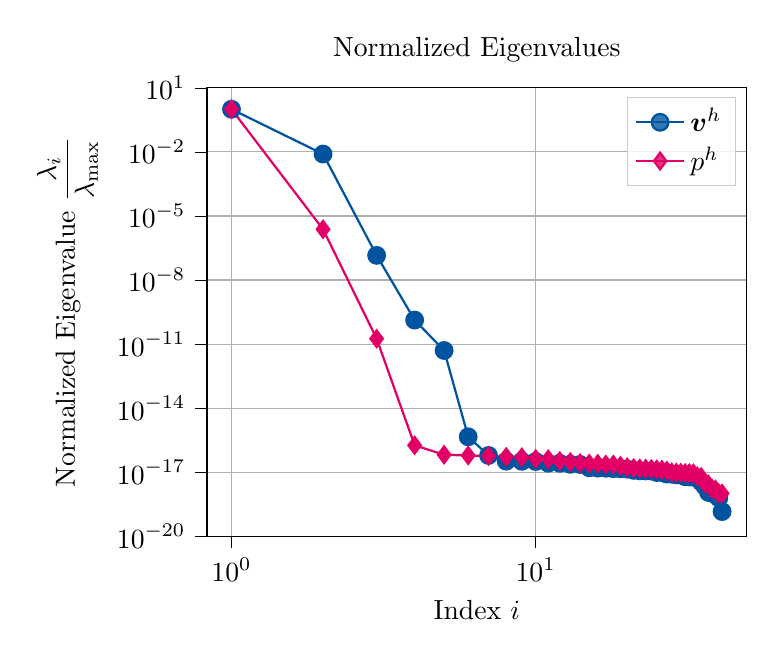
\begin{tikzpicture}

\definecolor{color0}{rgb}{0,0.329411764705882,0.623529411764706}
\definecolor{color1}{rgb}{0.890196078431372,0,0.4}

\begin{axis}[
legend cell align={left},
legend style={fill opacity=0.8, draw opacity=1, text opacity=1, draw=white!80!black},
log basis x={10},
log basis y={10},
tick align=outside,
tick pos=left,
title={Normalized Eigenvalues},
x grid style={white!69.0196078431373!black},
xlabel={Index \(\displaystyle i\)},
xmajorgrids,
xmin=0.830540485032707, xmax=49.3654442364545,
xmode=log,
xtick style={color=black},
xtick={0.01,0.1,1,10,100,1000},
xticklabels={
  \(\displaystyle 10^{-2}\),
  \(\displaystyle 10^{-1}\),
  \(\displaystyle 10^{0}\),
  \(\displaystyle 10^{1}\),
  \(\displaystyle 10^{2}\),
  \(\displaystyle 10^{3}\)
},
y grid style={white!69.0196078431373!black},
ylabel={Normalized Eigenvalue \(\displaystyle \frac{\lambda_i}{\lambda_{\text{max}}}\)},
ymajorgrids,
ymin=1e-20, ymax=10,
ymode=log,
ytick style={color=black},
ytick={1e-23,1e-20,1e-17,1e-14,1e-11,1e-08,1e-05,0.01,10,10000},
yticklabels={
  \(\displaystyle 10^{-23}\),
  \(\displaystyle 10^{-20}\),
  \(\displaystyle 10^{-17}\),
  \(\displaystyle 10^{-14}\),
  \(\displaystyle 10^{-11}\),
  \(\displaystyle 10^{-8}\),
  \(\displaystyle 10^{-5}\),
  \(\displaystyle 10^{-2}\),
  \(\displaystyle 10^{1}\),
  \(\displaystyle 10^{4}\)
}
]
\addplot [thick, color0, mark=*, mark size=3, mark options={solid}]
table {%
1 1
2 0.00794975858415845
3 1.42582257382325e-07
4 1.32791974403868e-10
5 5.00366283890635e-12
6 4.54114155240754e-16
7 6.04573529497411e-17
8 3.26201133022688e-17
9 3.22574638852698e-17
10 3.15358446366046e-17
11 2.62454621731955e-17
12 2.60840954654917e-17
13 2.33242093571454e-17
14 2.28813585566599e-17
15 1.60218882337199e-17
16 1.54306862706516e-17
17 1.52807821353466e-17
18 1.44864745846082e-17
19 1.43851705211444e-17
20 1.38677194525787e-17
21 1.21734236816605e-17
22 1.14897279038485e-17
23 1.13956935268721e-17
24 1.12564920102658e-17
25 9.63808041350083e-18
26 9.58979066065725e-18
27 8.13046505587439e-18
28 8.00740202533402e-18
29 7.46188080562777e-18
30 7.26718042554605e-18
31 6.11314351785897e-18
32 5.93273799548898e-18
33 5.84970067761768e-18
34 5.29939613242502e-18
35 3.47549460184894e-18
36 2.1905261247255e-18
37 1.12228744856004e-18
38 1.01406198292573e-18
39 9.59373162820783e-19
40 6.26226288149959e-19
41 1.42523827201686e-19
};
\addlegendentry{$\trialVelocityHomDiscrete$}
\addplot [thick, color1, mark=diamond*, mark size=3, mark options={solid}]
table {%
1 1
2 2.37328846603967e-06
3 1.78817929292869e-11
4 1.81154657334976e-16
5 6.51678466039161e-17
6 6.02235881107004e-17
7 5.69247083103718e-17
8 5.20065737906182e-17
9 5.01348143603465e-17
10 4.20958043774671e-17
11 4.07622974109276e-17
12 3.32697934377648e-17
13 2.98511733192585e-17
14 2.64421964531683e-17
15 2.52583071694472e-17
16 2.48386648445979e-17
17 2.27569426656641e-17
18 2.27247846357554e-17
19 1.99821382141988e-17
20 1.70491132142761e-17
21 1.54624364513944e-17
22 1.49112670601225e-17
23 1.45406520529215e-17
24 1.40935012359226e-17
25 1.35426769923973e-17
26 1.2976308799412e-17
27 1.18179500955933e-17
28 9.80114361457536e-18
29 9.51423374282225e-18
30 9.36239599182889e-18
31 9.08584610553105e-18
32 8.96571848518543e-18
33 8.78366822577326e-18
34 6.40001828288954e-18
35 5.93546015704658e-18
36 2.97856912325833e-18
37 2.64216217074413e-18
38 1.67829393129063e-18
39 1.53977850304594e-18
40 1.02797999983454e-18
41 1.00473640799576e-18
};
\addlegendentry{$p^h$}
\end{axis}

\end{tikzpicture}

        }
    }
    \subcaptionbox{Maximum interpolation error during the \gls{eim}.\label{fig:artery-likeEIMErrors}}{
        \resizebox{0.44\textwidth}{!}{
        % This file was created by tikzplotlib v0.9.8.
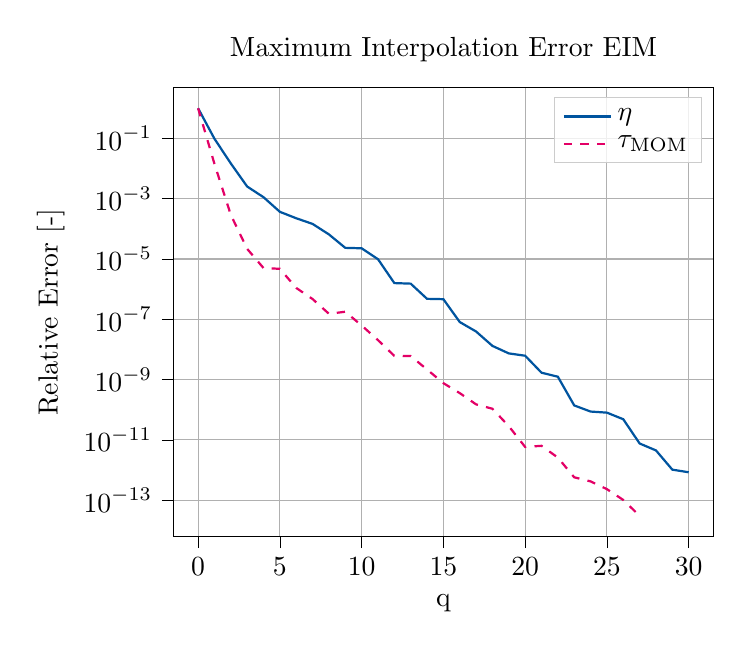
\begin{tikzpicture}

%\definecolor{color0}{rgb}{0.12156862745098,0.466666666666667,0.705882352941177}
%\definecolor{color1}{rgb}{1,0.498039215686275,0.0549019607843137}
\definecolor{color0}{rgb}{0,0.329411764705882,0.623529411764706}
\definecolor{color1}{rgb}{0.890196078431372,0,0.4}

\begin{axis}[
legend cell align={left},
legend style={fill opacity=0.8, draw opacity=1, text opacity=1, draw=white!80!black},
log basis y={10},
tick align=outside,
tick pos=left,
title={Maximum Interpolation Error EIM},
x grid style={white!69.0196078431373!black},
xlabel={q},
xmajorgrids,
xmin=-1.5, xmax=31.5,
xtick style={color=black},
xtick={-5,0,5,10,15,20,25,30,35},
xticklabels={
  \(\displaystyle -5\),
  \(\displaystyle 0\),
  \(\displaystyle 5\),
  \(\displaystyle 10\),
  \(\displaystyle 15\),
  \(\displaystyle 20\),
  \(\displaystyle 25\),
  \(\displaystyle 30\),
  \(\displaystyle 35\)
},
y grid style={white!69.0196078431373!black},
ylabel={Relative Error [-]},
ymajorgrids,
ymin=6.32307985340846e-15, ymax=4.74401718941179,
ymode=log,
ytick style={color=black},
ytick={1e-17,1e-15,1e-13,1e-11,1e-09,1e-07,1e-05,0.001,0.1,10,1000},
yticklabels={
  \(\displaystyle 10^{-17}\),
  \(\displaystyle 10^{-15}\),
  \(\displaystyle 10^{-13}\),
  \(\displaystyle 10^{-11}\),
  \(\displaystyle 10^{-9}\),
  \(\displaystyle 10^{-7}\),
  \(\displaystyle 10^{-5}\),
  \(\displaystyle 10^{-3}\),
  \(\displaystyle 10^{-1}\),
  \(\displaystyle 10^{1}\),
  \(\displaystyle 10^{3}\)
}
]
\addplot [thick, color0]
table {%
0 1
1 0.0973104687076621
2 0.0147633179066779
3 0.00252896805406514
4 0.00111793965375263
5 0.000366212967264887
6 0.000223970653068922
7 0.000145396874338459
8 6.52046804767942e-05
9 2.33321752580709e-05
10 2.26000046016262e-05
11 9.83915149206451e-06
12 1.58107750750885e-06
13 1.51597207604619e-06
14 4.75253511891816e-07
15 4.62299885501037e-07
16 8.06828170742323e-08
17 3.91006462079267e-08
18 1.30274119864675e-08
19 7.34041907118899e-09
20 6.15222072195395e-09
21 1.68400090499216e-09
22 1.23647681875085e-09
23 1.37973957655849e-10
24 8.64119044176524e-11
25 7.94881273897501e-11
26 4.80229695295645e-11
27 7.53378014734756e-12
28 4.43333366049816e-12
29 1.02026522151379e-12
30 8.36384533060246e-13
};
\addlegendentry{$\eta$}
\addplot [thick, color1, dashed]
table {%
0 1
1 0.0142591882104696
2 0.000290151916957558
3 2.16083662357261e-05
4 4.98689894693042e-06
5 4.70515968704204e-06
6 1.0922818762808e-06
7 4.67179954054551e-07
8 1.51464068402887e-07
9 1.77303957247854e-07
10 6.20554933265058e-08
11 2.02888056647836e-08
12 6.08014447268978e-09
13 5.99435297181841e-09
14 2.15022814619033e-09
15 7.55822336917672e-10
16 3.5378735937984e-10
17 1.49573256052504e-10
18 1.06992880868169e-10
19 2.82133502676071e-11
20 5.78225645869476e-12
21 6.30593569710007e-12
22 2.5585361244864e-12
23 5.685980701701e-13
24 4.16003286360201e-13
25 2.3040791442305e-13
26 1.00534473647095e-13
27 2.99967995145931e-14
};
\addlegendentry{$\tMomPlain$}
\end{axis}

\end{tikzpicture}

        }
    }
    \caption{Artery-like test case: results from the construction of the \gls{rom}.}
    \label{fig:artery-likeOffline}
\end{figure}
\par
\begin{figure}
    \captionsetup[sub]{position=bottom}
    \centering
    \Large
    \subcaptionbox{Velocity.}{
        \resizebox{0.44\textwidth}{!}{
        % This file was created by tikzplotlib v0.9.8.
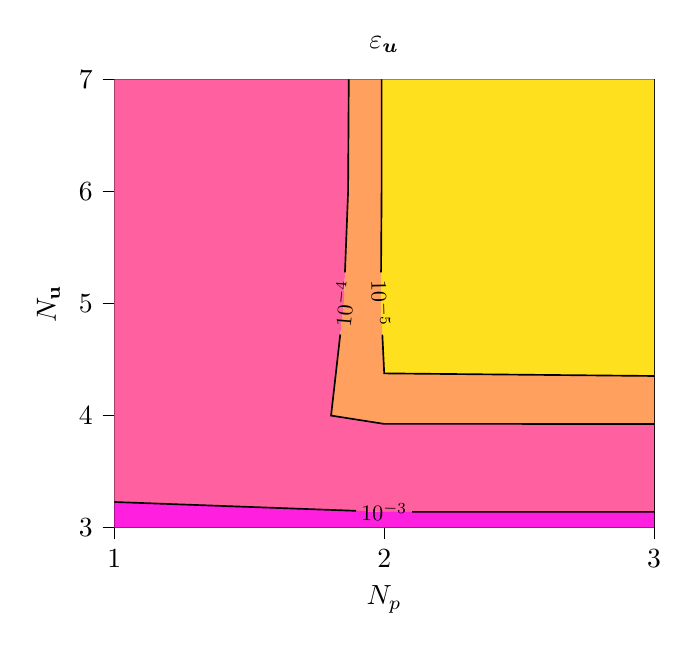
\begin{tikzpicture}

\definecolor{color0}{rgb}{1,0.87843137254902,0.12156862745098}
\definecolor{color1}{rgb}{1,0.627450980392157,0.372549019607843}
\definecolor{color2}{rgb}{1,0.376470588235294,0.623529411764706}
\definecolor{color3}{rgb}{1,0.125490196078431,0.874509803921569}

\begin{axis}[
tick align=outside,
tick pos=left,
%title={Relative Error in Velocity \(\displaystyle \mathbf{u}\) - Max},
title={$\relErrorVelocity$},
x grid style={white!69.0196078431373!black},
xlabel={\(\displaystyle N_p\)},
xmin=1, xmax=3,
xtick style={color=black},
xtick={1,2,3},
xticklabels={\(\displaystyle 1\),\(\displaystyle 2\),\(\displaystyle 3\)},
y grid style={white!69.0196078431373!black},
ylabel={\(\displaystyle N_{\mathbf{u}}\)},
ymin=3, ymax=7,
ytick style={color=black},
ytick={3,4,5,6,7},
yticklabels={
  \(\displaystyle 3\),
  \(\displaystyle 4\),
  \(\displaystyle 5\),
  \(\displaystyle 6\),
  \(\displaystyle 7\)
}
]
\addplot [draw=none, fill=color0]
table{%
x  y
2 4.37650891394412
3 4.35330770412385
3 5
3 6
3 7
2 7
1.99040991259345 7
1.9903127173998 6
1.98760845108052 5
2 4.37650891394412
};
\addplot [draw=none, fill=color1]
table{%
x  y
2 3.92579367910137
3 3.92540471448223
3 4
3 4.35330770412385
2 4.37650891394412
1.98760845108052 5
1.9903127173998 6
1.99040991259345 7
1.86869012295147 7
1.86619036626405 6
1.85013870710813 5
1.80309130655496 4
2 3.92579367910137
};
\addplot [draw=none, fill=color2]
table{%
x  y
2 3.14101234840689
3 3.14081265825156
3 3.92540471448223
2 3.92579367910137
1.80309130655496 4
1.85013870710813 5
1.86619036626405 6
1.86869012295147 7
1 7
1 6
1 5
1 4
1 3.22895886838152
2 3.14101234840689
};
\addplot [draw=none, fill=color3]
table{%
x  y
2 3
3 3
3 3.14081265825156
2 3.14101234840689
1 3.22895886838152
1 3
2 3
};
\path [draw=black, semithick]
(axis cs:3,4.35330770412385)
--(axis cs:2,4.37650891394412)
--(axis cs:1.99313704618645,4.72182414084339);

\path [draw=black, semithick]
(axis cs:1.98836176234379,5.27856400751013)
--(axis cs:1.9903127173998,6)
--(axis cs:1.99040991259345,7);

\path [draw=black, semithick]
(axis cs:3,3.92540471448223)
--(axis cs:2,3.92579367910137)
--(axis cs:1.80309130655496,4)
--(axis cs:1.83713590577805,4.72362338456115);

\path [draw=black, semithick]
(axis cs:1.85460609537104,5.27831317744237)
--(axis cs:1.86619036626405,6)
--(axis cs:1.86869012295147,7);

\path [draw=black, semithick]
(axis cs:3,3.14081265825156)
--(axis cs:2.10379029115697,3.14099162250753);

\path [draw=black, semithick]
(axis cs:1.89626538289669,3.15013544698203)
--(axis cs:1,3.22895886838152);

\draw (axis cs:1.98760845108052,5) node[
  scale=0.8,
  text=black,
  rotate=271.3
]{$10^{-5}$};
\draw (axis cs:1.85013870710813,5) node[
  scale=0.8,
  text=black,
  rotate=85.2
]{$10^{-4}$};
\draw (axis cs:2,3.14101234840689) node[
  scale=0.8,
  text=black,
  rotate=359.1
]{$10^{-3}$};
\end{axis}

\end{tikzpicture}
}
    }
    \subcaptionbox{Pressure.}{
        \resizebox{0.44\textwidth}{!}{
        % This file was created by tikzplotlib v0.9.8.
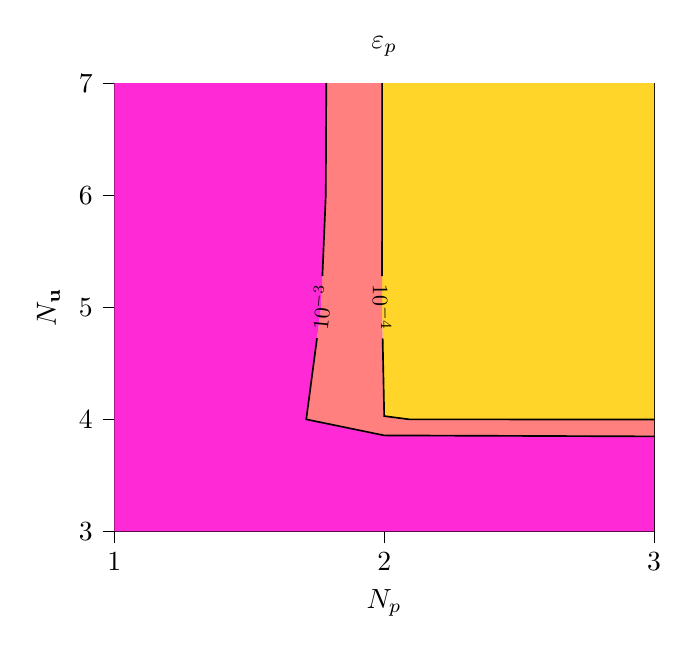
\begin{tikzpicture}

\definecolor{color0}{rgb}{1,0.835294117647059,0.164705882352941}
\definecolor{color1}{rgb}{1,0.501960784313725,0.498039215686275}
\definecolor{color2}{rgb}{1,0.164705882352941,0.835294117647059}

\begin{axis}[
tick align=outside,
tick pos=left,
%title={Relative Error in Pressure \(\displaystyle p\) - Max},
title={$\relErrorPressure$},
x grid style={white!69.0196078431373!black},
xlabel={\(\displaystyle N_p\)},
xmin=1, xmax=3,
xtick style={color=black},
xtick={1,2,3},
xticklabels={\(\displaystyle 1\),\(\displaystyle 2\),\(\displaystyle 3\)},
y grid style={white!69.0196078431373!black},
ylabel={\(\displaystyle N_{\mathbf{u}}\)},
ymin=3, ymax=7,
ytick style={color=black},
ytick={3,4,5,6,7},
yticklabels={
  \(\displaystyle 3\),
  \(\displaystyle 4\),
  \(\displaystyle 5\),
  \(\displaystyle 6\),
  \(\displaystyle 7\)
}
]
\addplot [draw=none, fill=color0]
table{%
x  y
3 3.99841272096808
3 4
3 5
3 6
3 7
2 7
1.99231388686608 7
1.9923086500537 6
1.99186016592534 5
2 4.02906689026844
2.0929081054864 4
3 3.99841272096808
};
\addplot [draw=none, fill=color1]
table{%
x  y
2 3.85666988114318
3 3.84783564712328
3 3.99841272096808
2.0929081054864 4
2 4.02906689026844
1.99186016592534 5
1.9923086500537 6
1.99231388686608 7
1.78528526361933 7
1.78346767600251 6
1.76616198020346 5
1.71107969290604 4
2 3.85666988114318
};
\addplot [draw=none, fill=color2]
table{%
x  y
2 3
3 3
3 3.84783564712328
2 3.85666988114318
1.71107969290604 4
1.76616198020346 5
1.78346767600251 6
1.78528526361933 7
1 7
1 6
1 5
1 4
1 3
2 3
};
\path [draw=black, semithick]
(axis cs:3,3.99841272096808)
--(axis cs:2.0929081054864,4)
--(axis cs:2,4.02906689026844)
--(axis cs:1.99419498249751,4.72149914921187);

\path [draw=black, semithick]
(axis cs:1.99198510066168,5.278571143184)
--(axis cs:1.9923086500537,6)
--(axis cs:1.99231388686608,7);

\path [draw=black, semithick]
(axis cs:3,3.84783564712328)
--(axis cs:2,3.85666988114318)
--(axis cs:1.71107969290604,4)
--(axis cs:1.75098262156661,4.72442395946829);

\path [draw=black, semithick]
(axis cs:1.77097765920204,5.27827133069329)
--(axis cs:1.78346767600251,6)
--(axis cs:1.78528526361933,7);

\draw (axis cs:1.99186016592534,5) node[
  scale=0.8,
  text=black,
  rotate=270.6
]{$10^{-4}$};
\draw (axis cs:1.76616198020346,5) node[
  scale=0.8,
  text=black,
  rotate=84.5
]{$10^{-3}$};
\end{axis}

\end{tikzpicture}
}
    }
    \caption{Artery-like test case: maximum relative error of the \gls{rom} over all testing samples.}
    \label{fig:artery-likeRelativeErrorMax}
\end{figure}
\par
Next, we present the results from the performance analysis. The \gls{rom} has been evaluated on a single core, whereas we have used 240 cores to compute the \gls{fom}. The measured speed up --- the average and the maximum over all the testing samples --- is shown in \Cref{fig:artery-likePerformance}. The results are, to some extent, counter-intuitive. First, one can observe that the speed up is mainly governed by $\nBasisVelocityROM$ and roughly constant for  $\nBasisPressureROM$. Second, the speed up does not change monotonically with increasing $\nBasisVelocityROM$ but has a local maximum at $\nBasisVelocityROM=5$. Analyzing the evaluation of the \gls{rom} in more detail has revealed that this pattern originates from the number of iterations needed to solve the non-linear reduced system. In particular, the value for $\nBasisVelocityROM$ influences the number of non-linear iterations and, in some cases, slows down the solution process. Nevertheless, the order of magnitude of the observed speed up, ranging from 25,000 to 60,000, is still compelling and even much more significant than in the previous test case.
\begin{figure}
    \captionsetup[sub]{position=bottom}
    \centering
    \Large
    \subcaptionbox{Average speed up over all testing samples.}{
        \resizebox{0.44\textwidth}{!}{
        % This file was created by tikzplotlib v0.9.8.
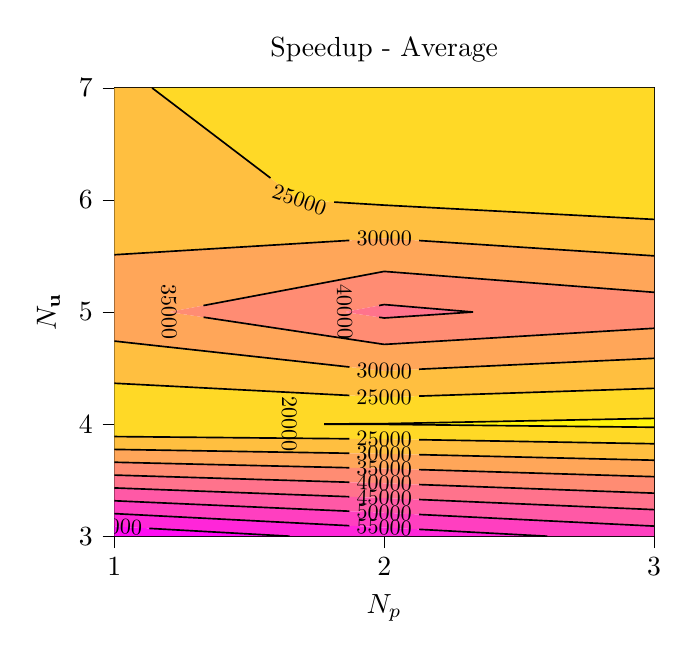
\begin{tikzpicture}

\definecolor{color0}{rgb}{1,0.952941176470588,0.0470588235294118}
\definecolor{color1}{rgb}{1,0.850980392156863,0.149019607843137}
\definecolor{color2}{rgb}{1,0.749019607843137,0.250980392156863}
\definecolor{color3}{rgb}{1,0.650980392156863,0.349019607843137}
\definecolor{color4}{rgb}{1,0.549019607843137,0.450980392156863}
\definecolor{color5}{rgb}{1,0.450980392156863,0.549019607843137}
\definecolor{color6}{rgb}{1,0.349019607843137,0.650980392156863}
\definecolor{color7}{rgb}{1,0.247058823529412,0.752941176470588}
\definecolor{color8}{rgb}{1,0.149019607843137,0.850980392156863}
\definecolor{color9}{rgb}{1,0.0470588235294118,0.952941176470588}

\begin{axis}[
tick align=outside,
tick pos=left,
title={Speedup - Average},
x grid style={white!69.0196078431373!black},
xlabel={\(\displaystyle N_p\)},
xmin=1, xmax=3,
xtick style={color=black},
xtick={1,2,3},
xticklabels={\(\displaystyle 1\),\(\displaystyle 2\),\(\displaystyle 3\)},
y grid style={white!69.0196078431373!black},
ylabel={\(\displaystyle N_{\mathbf{u}}\)},
ymin=3, ymax=7,
ytick style={color=black},
ytick={3,4,5,6,7},
yticklabels={
  \(\displaystyle 3\),
  \(\displaystyle 4\),
  \(\displaystyle 5\),
  \(\displaystyle 6\),
  \(\displaystyle 7\)
}
]
\addplot [draw=none, fill=color0]
table{%
x  y
2 3.99776029877739
3 3.97186061500088
3 4
3 4.05129247948725
2 4.00401665310977
1.64783776122399 4
2 3.99776029877739
};
\addplot [draw=none, fill=color1]
table{%
x  y
2 3.86632751738316
3 3.82489079580478
3 3.97186061500088
2 3.99776029877739
1.64783776122399 4
2 4.00401665310977
3 4.05129247948725
3 4.31918911036938
2 4.23972661512697
1 4.36447852644752
1 4
1 3.88899847255399
2 3.86632751738316
};
\addplot [draw=none, fill=color1]
table{%
x  y
2 5.95377752187074
3 5.82647002301902
3 6
3 7
2 7
1.13955470147603 7
1.68538959041588 6
2 5.95377752187074
};
\addplot [draw=none, fill=color2]
table{%
x  y
2 3.73489473598894
3 3.67792097660869
3 3.82489079580478
2 3.86632751738316
1 3.88899847255399
1 3.77440465802077
2 3.73489473598894
};
\addplot [draw=none, fill=color2]
table{%
x  y
2 4.23972661512697
3 4.31918911036938
3 4.58708574125151
2 4.47543657714418
1 4.74075248971692
1 4.36447852644752
2 4.23972661512697
};
\addplot [draw=none, fill=color2]
table{%
x  y
2 5.65807486026756
3 5.50125704822069
3 5.82647002301902
2 5.95377752187074
1.68538959041588 6
1.13955470147603 7
1 7
1 6
1 5.51094647432634
2 5.65807486026756
};
\addplot [draw=none, fill=color3]
table{%
x  y
2 3.60346195459471
3 3.5309511574126
3 3.67792097660869
2 3.73489473598894
1 3.77440465802077
1 3.65981084348756
2 3.60346195459471
};
\addplot [draw=none, fill=color3]
table{%
x  y
2 4.47543657714418
3 4.58708574125151
3 4.85498237213365
2 4.71114653916139
1.20242039825908 5
2 5.36237219866437
3 5.17604407342235
3 5.50125704822069
2 5.65807486026756
1 5.51094647432634
1 5
1 4.74075248971692
2 4.47543657714418
};
\addplot [draw=none, fill=color4]
table{%
x  y
2 3.47202917320049
3 3.38398133821651
3 3.5309511574126
2 3.60346195459471
1 3.65981084348756
1 3.54521702895434
2 3.47202917320049
};
\addplot [draw=none, fill=color4]
table{%
x  y
2 4.71114653916139
3 4.85498237213365
3 5
3 5.17604407342235
2 5.36237219866437
1.20242039825908 5
2 4.71114653916139
1.85326064468108 5
2 5.06666953706118
2.3295534889383 5
2 4.94685650117859
1.85326064468108 5
};
\addplot [draw=none, fill=color5]
table{%
x  y
2 3.34059639180626
3 3.23701151902041
3 3.38398133821651
2 3.47202917320049
1 3.54521702895434
1 3.43062321442112
2 3.34059639180626
};
\addplot [draw=none, fill=color5]
table{%
x  y
2 4.94685650117859
2.3295534889383 5
2 5.06666953706118
1.85326064468108 5
2 4.94685650117859
};
\addplot [draw=none, fill=color6]
table{%
x  y
2 3.20916361041203
3 3.09004169982432
3 3.23701151902041
2 3.34059639180626
1 3.43062321442112
1 3.3160293998879
2 3.20916361041203
};
\addplot [draw=none, fill=color7]
table{%
x  y
2 3.07773082901781
2.60424735056556 3
3 3
3 3.09004169982432
2 3.20916361041203
1 3.3160293998879
1 3.20143558535469
2 3.07773082901781
};
\addplot [draw=none, fill=color8]
table{%
x  y
2 3
2.60424735056556 3
2 3.07773082901781
1 3.20143558535469
1 3.08684177082147
1.64970439596316 3
2 3
};
\addplot [draw=none, fill=color9]
table{%
x  y
1 3.08684177082147
1 3
1.64970439596316 3
1 3.08684177082147
};
\path [draw=black, semithick]
(axis cs:3,3.97186061500088)
--(axis cs:2,3.99776029877739)
--(axis cs:1.77726149904818,3.99917688362941);

\path [draw=black, semithick]
(axis cs:1.77726069380053,4.00147615776869)
--(axis cs:2,4.00401665310977)
--(axis cs:3,4.05129247948725);

\path [draw=black, semithick]
(axis cs:3,3.82489079580478)
--(axis cs:2.12940867994302,3.86096524594254);

\path [draw=black, semithick]
(axis cs:1.87058051564284,3.86926158071125)
--(axis cs:1,3.88899847255399);

\path [draw=black, semithick]
(axis cs:1,4.36447852644752)
--(axis cs:1.87071547689406,4.2558551064886);

\path [draw=black, semithick]
(axis cs:2.12936741661236,4.25000647285406)
--(axis cs:3,4.31918911036938);

\path [draw=black, semithick]
(axis cs:3,5.82647002301902)
--(axis cs:2,5.95377752187074)
--(axis cs:1.81462022259509,5.98101346971504);

\path [draw=black, semithick]
(axis cs:1.57849420274952,6.1958383200348)
--(axis cs:1.13955470147603,7);

\path [draw=black, semithick]
(axis cs:3,3.67792097660869)
--(axis cs:2.1293949518265,3.72752261913855);

\path [draw=black, semithick]
(axis cs:1.87058991946085,3.74000771818117)
--(axis cs:1,3.77440465802077);

\path [draw=black, semithick]
(axis cs:1,4.74075248971692)
--(axis cs:1.87120364443596,4.5096082997567);

\path [draw=black, semithick]
(axis cs:2.12931226725914,4.48987418369249)
--(axis cs:3,4.58708574125151);

\path [draw=black, semithick]
(axis cs:3,5.50125704822069)
--(axis cs:2.12920375458042,5.63781341016601);

\path [draw=black, semithick]
(axis cs:1.87076991649158,5.63906144666591)
--(axis cs:1,5.51094647432634);

\path [draw=black, semithick]
(axis cs:3,3.5309511574126)
--(axis cs:2.12937689557672,3.5940807327595);

\path [draw=black, semithick]
(axis cs:1.87060441248816,3.61075325217864)
--(axis cs:1,3.65981084348756);

\path [draw=black, semithick]
(axis cs:3,5.17604407342235)
--(axis cs:2,5.36237219866437)
--(axis cs:1.33002909148532,5.05797771486651);

\path [draw=black, semithick]
(axis cs:1.33068211116719,4.95354841123603)
--(axis cs:2,4.71114653916139)
--(axis cs:3,4.85498237213365);

\path [draw=black, semithick]
(axis cs:3,3.38398133821651)
--(axis cs:2.12935451663035,3.46063978806578);

\path [draw=black, semithick]
(axis cs:1.87062398959549,3.48149792598798)
--(axis cs:1,3.54521702895434);

\path [draw=black, semithick]
(axis cs:1.98152235758919,4.95354841123603)
--(axis cs:2,4.94685650117859)
--(axis cs:2.3295534889383,5)
--(axis cs:2,5.06666953706118)
--(axis cs:1.98086933790731,5.05797771486651);

\path [draw=black, semithick]
(axis cs:3,3.23701151902041)
--(axis cs:2.12932782172,3.32719998584572);

\path [draw=black, semithick]
(axis cs:1.87064864385909,3.35224148340055)
--(axis cs:1,3.43062321442112);

\path [draw=black, semithick]
(axis cs:3,3.09004169982432)
--(axis cs:2.12929681886861,3.19376152631549);

\path [draw=black, semithick]
(axis cs:1.87067836656755,3.2229836688651)
--(axis cs:1,3.3160293998879);

\path [draw=black, semithick]
(axis cs:2.60424735056556,3)
--(axis cs:2.12927570066499,3.06110070664302);

\path [draw=black, semithick]
(axis cs:1.87071314723031,3.09372422763725)
--(axis cs:1,3.20143558535469);

\path [draw=black, semithick]
(axis cs:1.64970439596316,3)
--(axis cs:1.12926390778472,3.06956390303255);

\draw (axis cs:1.64783776122399,4) node[
  scale=0.8,
  text=black,
  rotate=270.1
]{20000};
\draw (axis cs:2,3.86632751738316) node[
  scale=0.8,
  text=black,
  rotate=359.3
]{25000};
\draw (axis cs:2,4.23972661512697) node[
  scale=0.8,
  text=black,
  rotate=359.5
]{25000};
\draw (axis cs:1.68538959041588,6) node[
  scale=0.8,
  text=black,
  rotate=341.3
]{25000};
\draw (axis cs:2,3.73489473598894) node[
  scale=0.8,
  text=black,
  rotate=359.0
]{30000};
\draw (axis cs:2,4.47543657714418) node[
  scale=0.8,
  text=black,
  rotate=358.4
]{30000};
\draw (axis cs:2,5.65807486026756) node[
  scale=0.8,
  text=black,
  rotate=359.9
]{30000};
\draw (axis cs:2,3.60346195459471) node[
  scale=0.8,
  text=black,
  rotate=358.6
]{35000};
\draw (axis cs:1.20242039825908,5) node[
  scale=0.8,
  text=black,
  rotate=271.0
]{35000};
\draw (axis cs:2,3.47202917320049) node[
  scale=0.8,
  text=black,
  rotate=358.3
]{40000};
\draw (axis cs:1.85326064468108,5) node[
  scale=0.8,
  text=black,
  rotate=271.0
]{40000};
\draw (axis cs:2,3.34059639180626) node[
  scale=0.8,
  text=black,
  rotate=357.9
]{45000};
\draw (axis cs:2,3.20916361041203) node[
  scale=0.8,
  text=black,
  rotate=357.6
]{50000};
\draw (axis cs:2,3.07773082901781) node[
  scale=0.8,
  text=black,
  rotate=357.3
]{55000};
\draw (axis cs:1,3.08684177082147) node[
  scale=0.8,
  text=black,
  rotate=357.1
]{60000};
\end{axis}

\end{tikzpicture}
}
    }
    \subcaptionbox{Maximum speed up over all testing samples.}{
        \resizebox{0.44\textwidth}{!}{
        % This file was created by tikzplotlib v0.9.8.
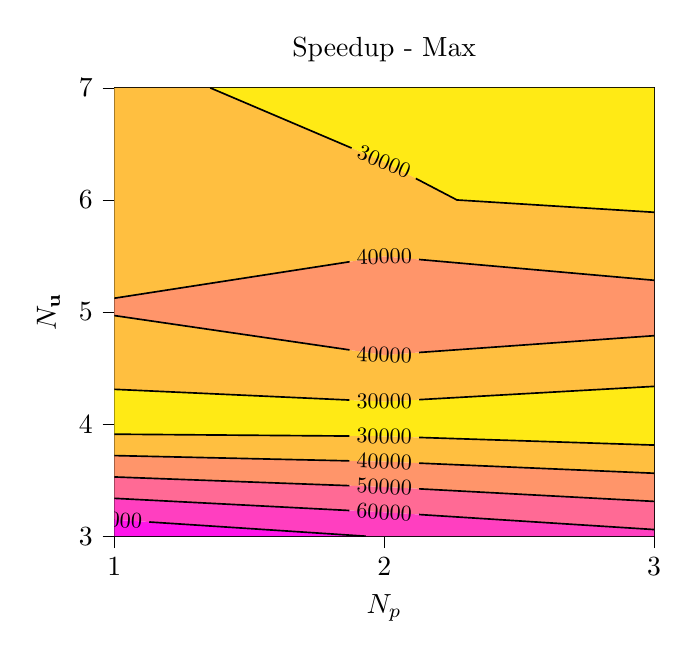
\begin{tikzpicture}

\definecolor{color0}{rgb}{1,0.917647058823529,0.0823529411764706}
\definecolor{color1}{rgb}{1,0.749019607843137,0.250980392156863}
\definecolor{color2}{rgb}{1,0.584313725490196,0.415686274509804}
\definecolor{color3}{rgb}{1,0.415686274509804,0.584313725490196}
\definecolor{color4}{rgb}{1,0.247058823529412,0.752941176470588}
\definecolor{color5}{rgb}{1,0.0823529411764706,0.917647058823529}

\begin{axis}[
tick align=outside,
tick pos=left,
title={Speedup - Max},
x grid style={white!69.0196078431373!black},
xlabel={\(\displaystyle N_p\)},
xmin=1, xmax=3,
xtick style={color=black},
xtick={1,2,3},
xticklabels={\(\displaystyle 1\),\(\displaystyle 2\),\(\displaystyle 3\)},
y grid style={white!69.0196078431373!black},
ylabel={\(\displaystyle N_{\mathbf{u}}\)},
ymin=3, ymax=7,
ytick style={color=black},
ytick={3,4,5,6,7},
yticklabels={
  \(\displaystyle 3\),
  \(\displaystyle 4\),
  \(\displaystyle 5\),
  \(\displaystyle 6\),
  \(\displaystyle 7\)
}
]
\addplot [draw=none, fill=color0]
table{%
x  y
2 3.89113969366561
3 3.81295761379902
3 4
3 4.33664393194555
2 4.20059943824401
1 4.31046717020061
1 4
1 3.91000519290614
2 3.89113969366561
};
\addplot [draw=none, fill=color0]
table{%
x  y
3 5.8901285826523
3 6
3 7
2 7
1.35534430289395 7
2 6.33923453361608
2.26948248989546 6
3 5.8901285826523
};
\addplot [draw=none, fill=color1]
table{%
x  y
2 3.66515692779255
3 3.56174755756104
3 3.81295761379902
2 3.89113969366561
1 3.91000519290614
1 3.71929144543007
2 3.66515692779255
};
\addplot [draw=none, fill=color1]
table{%
x  y
2 4.20059943824401
3 4.33664393194555
3 4.78877856727545
2 4.61702317811216
1 4.96839799320352
1 4.31046717020061
2 4.20059943824401
};
\addplot [draw=none, fill=color1]
table{%
x  y
2 5.49635319629926
3 5.28342883044444
3 5.8901285826523
2.26948248989546 6
2 6.33923453361608
1.35534430289395 7
1 7
1 6
1 5.12326574274158
2 5.49635319629926
};
\addplot [draw=none, fill=color2]
table{%
x  y
2 3.4391741619195
3 3.31053750132306
3 3.56174755756104
2 3.66515692779255
1 3.71929144543007
1 3.52857769795399
2 3.4391741619195
};
\addplot [draw=none, fill=color2]
table{%
x  y
2 4.61702317811216
3 4.78877856727545
3 5
3 5.28342883044444
2 5.49635319629926
1 5.12326574274158
1 5
1 4.96839799320352
2 4.61702317811216
};
\addplot [draw=none, fill=color3]
table{%
x  y
2 3.21319139604645
3 3.05932744508508
3 3.31053750132306
2 3.4391741619195
1 3.52857769795399
1 3.33786395047791
2 3.21319139604645
};
\addplot [draw=none, fill=color4]
table{%
x  y
2 3
3 3
3 3.05932744508508
2 3.21319139604645
1 3.33786395047791
1 3.14715020300184
1.93165335182826 3
2 3
};
\addplot [draw=none, fill=color5]
table{%
x  y
1 3.14715020300184
1 3
1.93165335182826 3
1 3.14715020300184
};
\path [draw=black, semithick]
(axis cs:3,3.81295761379902)
--(axis cs:2.12936922751048,3.8810253383881);

\path [draw=black, semithick]
(axis cs:1.87057909585802,3.89358128363441)
--(axis cs:1,3.91000519290614);

\path [draw=black, semithick]
(axis cs:1,4.31046717020061)
--(axis cs:1.87068419689434,4.21480707223737);

\path [draw=black, semithick]
(axis cs:2.12925816089073,4.21818429929918)
--(axis cs:3,4.33664393194555);

\path [draw=black, semithick]
(axis cs:3,5.8901285826523)
--(axis cs:2.26948248989546,6)
--(axis cs:2.11717612375158,6.19172889157148);

\path [draw=black, semithick]
(axis cs:1.87909257266006,6.46316340444465)
--(axis cs:1.35534430289395,7);

\path [draw=black, semithick]
(axis cs:3,3.56174755756104)
--(axis cs:2.12932814733133,3.65178318552381);

\path [draw=black, semithick]
(axis cs:1.87060221616005,3.67216181440409)
--(axis cs:1,3.71929144543007);

\path [draw=black, semithick]
(axis cs:1,4.96839799320352)
--(axis cs:1.87167093357662,4.66211478009752);

\path [draw=black, semithick]
(axis cs:2.12915991192253,4.63920708904871)
--(axis cs:3,4.78877856727545);

\path [draw=black, semithick]
(axis cs:3,5.28342883044444)
--(axis cs:2.12901874905936,5.46888196097241);

\path [draw=black, semithick]
(axis cs:1.87180845969371,5.44852654095875)
--(axis cs:1,5.12326574274158);

\path [draw=black, semithick]
(axis cs:3,3.31053750132306)
--(axis cs:2.12927571007098,3.42254456627974);

\path [draw=black, semithick]
(axis cs:1.87064764090286,3.45073872021719)
--(axis cs:1,3.52857769795399);

\path [draw=black, semithick]
(axis cs:3,3.05932744508508)
--(axis cs:2.12921195720541,3.19331033379938);

\path [draw=black, semithick]
(axis cs:1.87071529966112,3.22930964988661)
--(axis cs:1,3.33786395047791);

\path [draw=black, semithick]
(axis cs:1.93165335182826,3)
--(axis cs:1.12920058312662,3.12674358717447);

\draw (axis cs:2,3.89113969366561) node[
  scale=0.8,
  text=black,
  rotate=359.0
]{30000};
\draw (axis cs:2,4.20059943824401) node[
  scale=0.8,
  text=black,
  rotate=0.3
]{30000};
\draw (axis cs:2,6.33923453361608) node[
  scale=0.8,
  text=black,
  rotate=337.0
]{30000};
\draw (axis cs:2,3.66515692779255) node[
  scale=0.8,
  text=black,
  rotate=358.3
]{40000};
\draw (axis cs:2,4.61702317811216) node[
  scale=0.8,
  text=black,
  rotate=358.1
]{40000};
\draw (axis cs:2,5.49635319629926) node[
  scale=0.8,
  text=black,
  rotate=1.7
]{40000};
\draw (axis cs:2,3.4391741619195) node[
  scale=0.8,
  text=black,
  rotate=357.7
]{50000};
\draw (axis cs:2,3.21319139604645) node[
  scale=0.8,
  text=black,
  rotate=357.0
]{60000};
\draw (axis cs:1,3.14715020300184) node[
  scale=0.8,
  text=black,
  rotate=356.6
]{70000};
\end{axis}

\end{tikzpicture}
}
    }
    \caption{Artery-like test case: performance results.}
    \label{fig:artery-likePerformance}
\end{figure}
\par
So, also the results for this test case underline the advantages of the proposed approach in general and, specifically, its ability to handle problems defined in a four-dimensional space-time domain. 

\section{Conclusion}
\label{sec:conclusion}
\section{Conclusion}\label{sec:conclusion}
In this work, we focus on addressing the fundamental challenge of OOD detection tasks, which is how to fully understand the semantic discrepancy between the ID/OOD samples. We reveal that the key to success in the realistic SCOOD task is to allocate as many ID samples in the unlabeled set correctly as possible. To this end, we propose a novel uncertainty-aware optimal transport scheme that introduces class-specific energy scores as guidance for effective label assignment. Experimental results show that our method achieves better performance than previous state-of-the-art methods on SCOOD benchmarks.

\textbf{Limitations.} In addition to temperature scaling, other techniques such as feature clipping applied in ReAct~\cite{sun2021react} also enhance the performance of energy score, so how to obtain an OOD score that best fits the SCOOD task can be further explored. Moreover, a setting highly related to SCOOD has been proposed in \cite{katz2022training} and formulated as a constrained optimization problem. We will also theoretically analyze these practical OOD settings in our feature work.

% \section*{Acknowledgments}
\textbf{Acknowledgments.} 
This work is supported by National Key R\&D Program of China under Grant 2020AAA0105701, National Natural Science Foundation of China (NSFC) under Grants 61872327, Major Special Science and Technology Project of Anhui, National Natural Science Foundation of China (62033012) and Ant Group through Ant Research Intern Program.

\section*{Acknowledgments}
\label{sec:acknowledgments}
% Acknowledgments---Will not appear in anonymized version
\midlacknowledgments{We would like to thank Dr. Birgit Stierstorfer (Non Clinical Drug Safety, Boehringer Ingelheim, Biberach, Germany) and Dr. Charlotte Lempp (Drug Discovery Sciences, Boehringer Ingelheim, Biberach, Germany)
for their help with the visual evaluation of the artificially generated images and Dr. Martin Lenter (Drug
Discovery Sciences, Boehringer Ingelheim, Biberach, Germany) for helpful discussions and project support. We would also
like to thank Dr. Lina Humbeck (Medicinal Chemistry,
Boehringer Ingelheim, Biberach, Germany) for her comments,
which helped to improve the quality of the paper.}

\printbibliography

\end{document}
